\documentclass{article} % ICLR 2026

\usepackage{iclr2026_conference,times}
\usepackage[T1]{fontenc}

\usepackage{graphicx}%
\usepackage{multirow}%
\usepackage{amsmath,amssymb,amsfonts}%
\usepackage{amsthm}%
\usepackage[title]{appendix}%
\usepackage{xcolor}%
\usepackage{textcomp}%
\usepackage{booktabs}%

%  ==================== MY PACKAGES ====================
\usepackage{acronym}
\usepackage{tabularx}
\usepackage{fancyvrb}
\usepackage{hyperref}
\usepackage{url}
\usepackage{enumitem}
\usepackage{colortbl}
\usepackage{siunitx}

\setlist[enumerate]{noitemsep, nosep}
\setlist[itemize]{noitemsep, nosep}

%  ==================== MY COMMANDS ====================
\theoremstyle{definition}

\newtheorem{definition}{Definition}
\newtheorem{hypothesis}{Hypothesis}

\theoremstyle{plain}
\newtheorem{finding}{Finding}

\newtheorem*{researchquestion}{RQ}

\newcommand{\librarylink}{ \url{https://anonymous.4open.science/r/apunim-5F70}}
\newcommand{\doclink}{\url{https://anonymous.4open.science/r/apunim-page}}
\newcommand{\explink}{\url{https://anonymous.4open.science/r/aposteriori-unimodality-E8C1}}

\newcommand\given[1][]{\:#1\vert\:}

\graphicspath{ {../graphs} {graphs}  }

\title{Are We Chasing Shadows? Quantifying Unattributable Polarization\\and Attributing the Rest to Annotator Groups}

\author{Anonymous}
\begin{document}

\maketitle

\begin{abstract}
	Polarization has recently been proposed as a robust way of distinguishing minor disagreements from systematic differences in opinion for imbalanced, minority groups but there currently exists no methodology for attributing polarization to these groups. In this study, we discover and investigate two major limitations in realistic settings: (1) the presence of ``inherent'' polarization that cannot be attributed to any known or latent groups, and (2) opposing polarization effects canceling each other out in aggregated annotations. To address these issues, we introduce a new metric that attributes polarization to any annotator group while avoiding these limitations, tailored to smaller datasets common in NLP, and provide an open-source Python library implementation. We apply our method to four content moderation datasets and confirm that gender and ethnicity consistently explain polarization patterns, while ideology and personal experiences may be more important than previously thought. Our work overall indicates that subjective NLP datasets may need fewer items and more annotators per item.
\end{abstract}


\section{Introduction}
\label{sec:intro}



Annotations are essential for subjective tasks, such as content moderation, toxicity, and \acf{hs} detection, which are especially important for protecting minority groups~\cite{un_hate_speech_targets, ucdavis_hate_speech}. However, in practice, analysis rests on inter-annotator agreement or majority-vote~\cite{ivey-etal-2025-nutmeg, petra_2022_handling, van_der_Velden}, which may lead to biased and misconfigured systems (e.g., toxicity models disproportionally marking \ac{aa} speech as ``toxic''~\cite{sap-etal-2019-risk}), or discard \emph{fundamental} disagreements between minority groups and the majority~\cite{quaranto2022dog}, (see the example in Fig.~\ref{fig:disagreement-vs-polarization}).\footnote{The simulated experiments in this study were implemented by generating random annotations following the normal distribution with differing means and \ac{sd}---see App.~\ref{app:experiments}.}

\begin{figure}[ht]
	\centering
	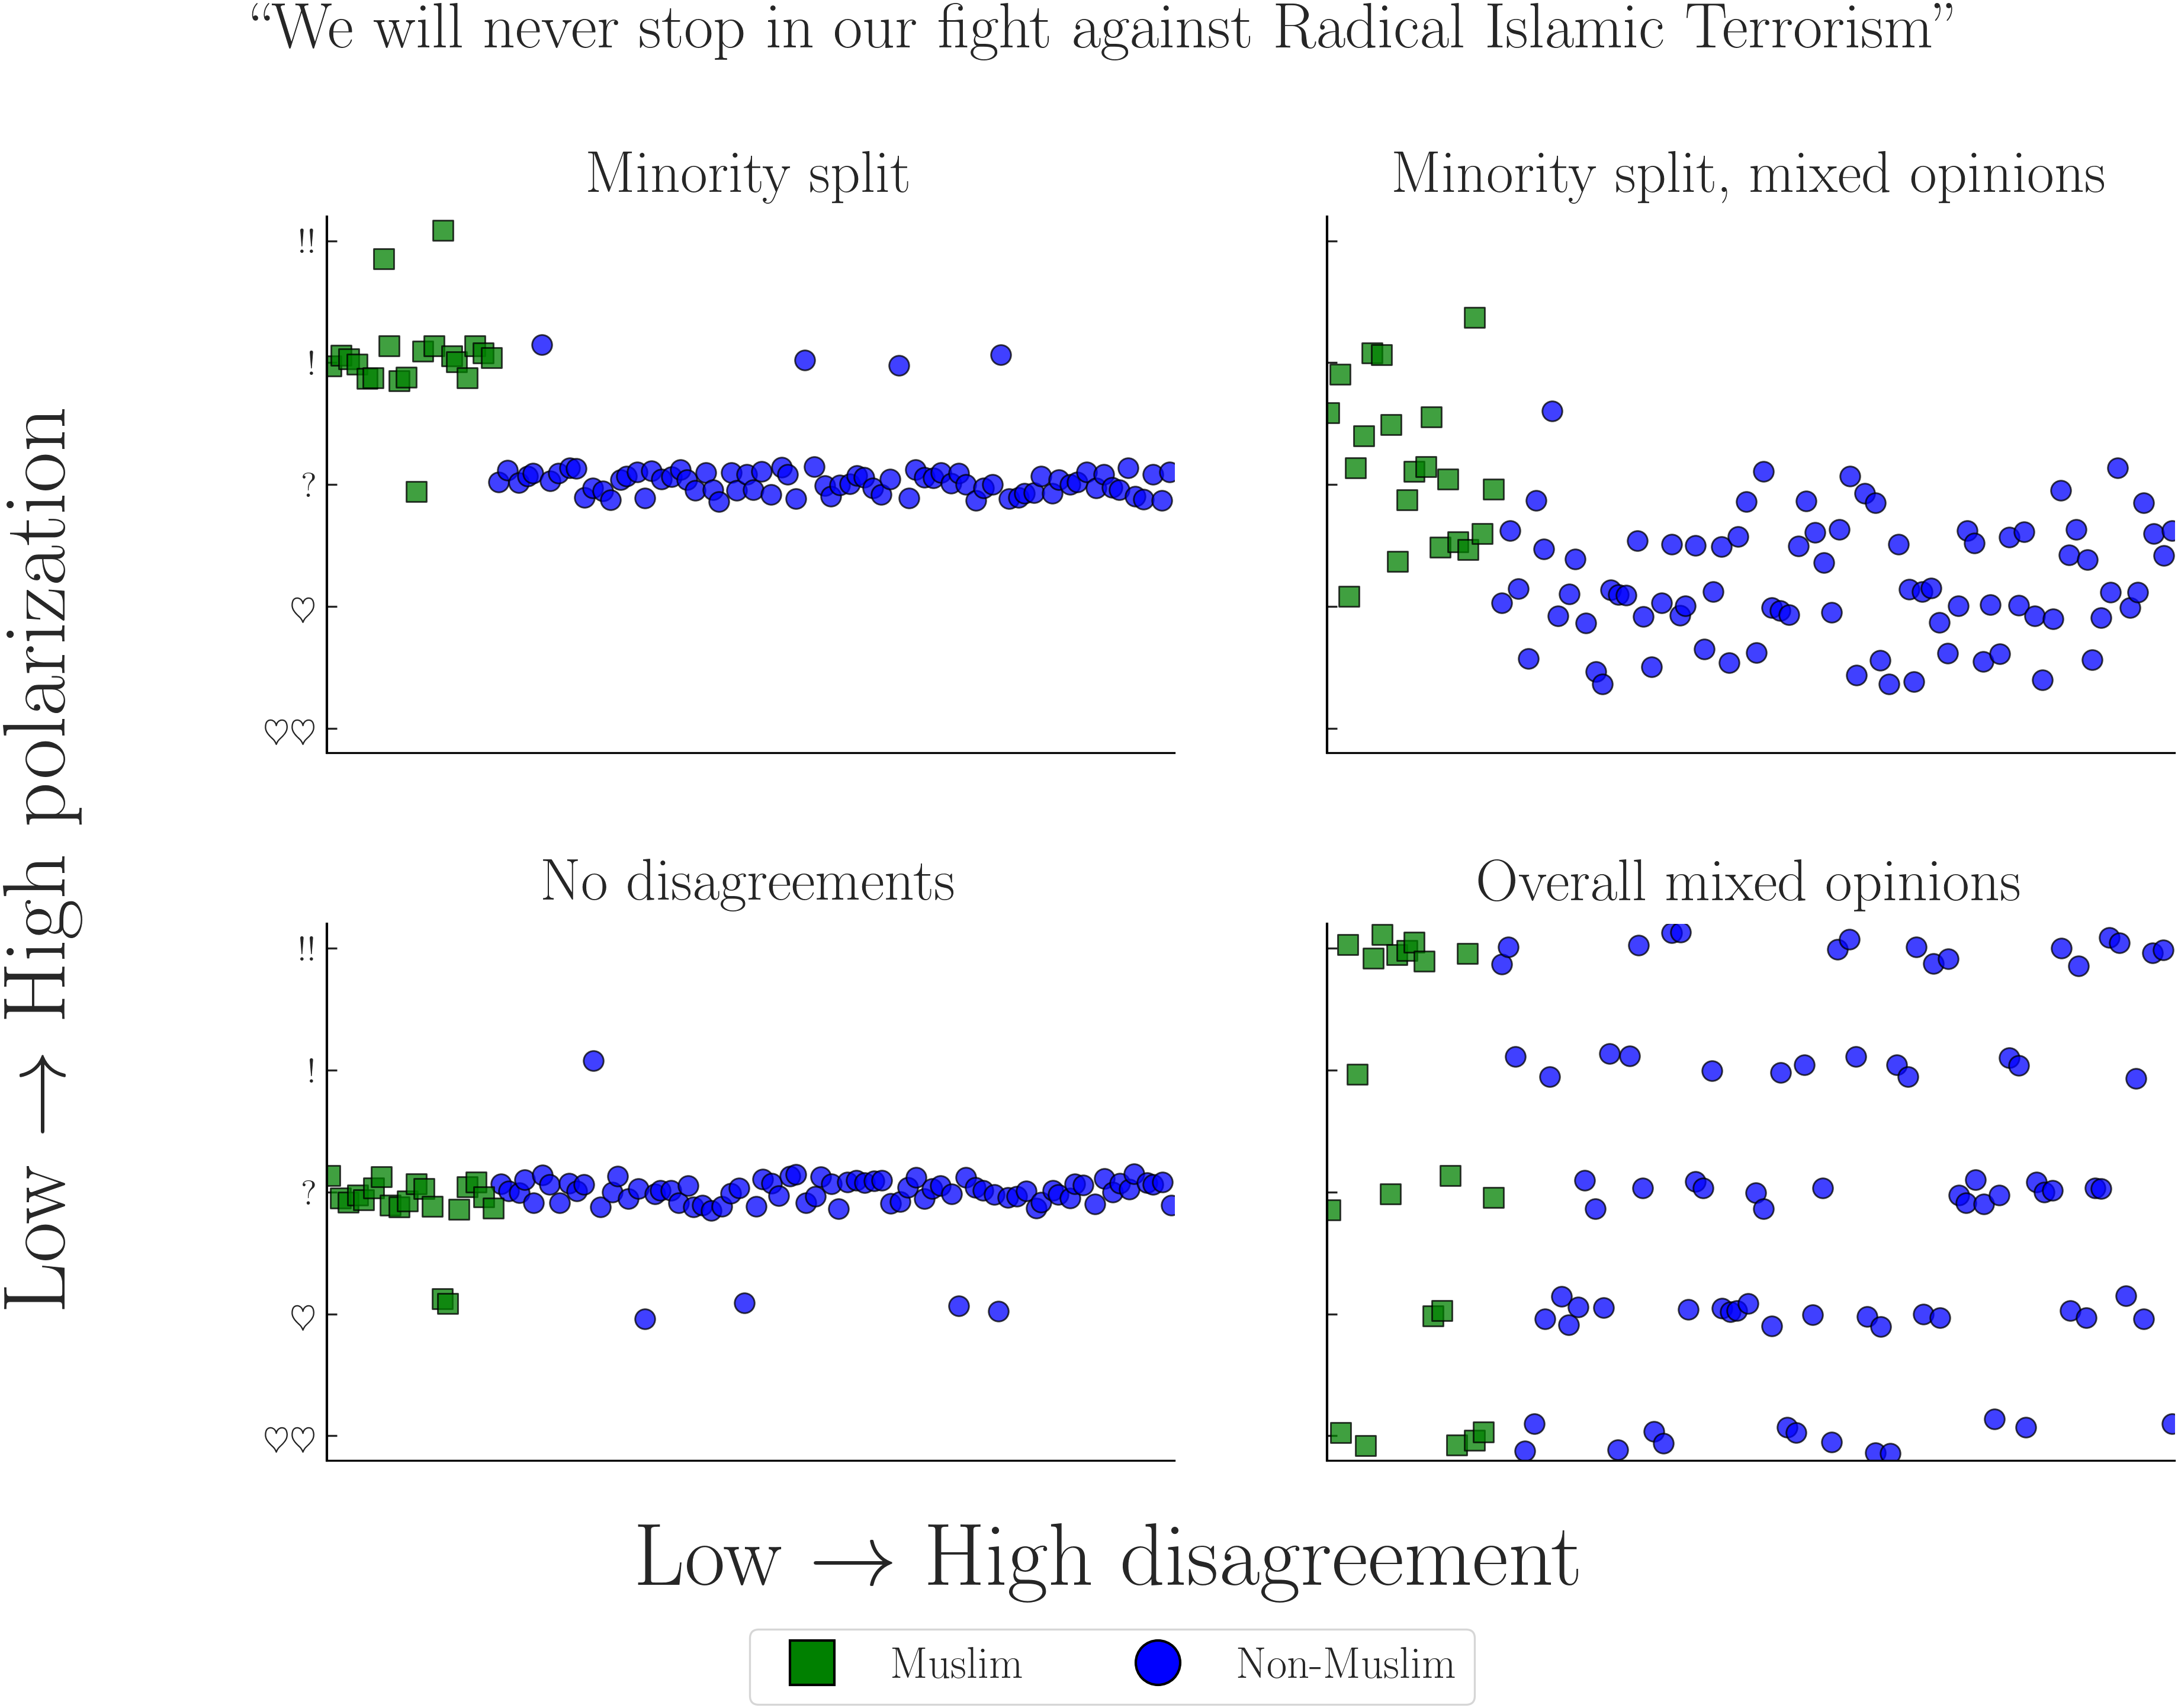
\includegraphics[width=0.55\textwidth]{disagreement_vs_polarization.png}
	\caption{Simulated experiment exploring four scenarios of a \ac{hs} detection task applied to a controversial statement by D. Trump (Jan. 2019). The variance in annotations across different annotators may cause traditional agreement metrics to ignore minority opinions, especially when opinions are mixed (top-right).}
	\label{fig:disagreement-vs-polarization}
\end{figure}

One alternative is using \emph{polarization}, which correlates better with human judgments and is much less sensitive to different group sizes \cite{Pavlopoulos2023, pavlopoulos-likas-2024}. While we can detect polarization, there is little work on how to detect whether it is \emph{actually caused by marginalized groups}. Our work thus tries to answer the following Research Question (RQ):

\begin{researchquestion}[]
	How much polarization can we practically attribute to annotator subgroups given existing datasets?
\end{researchquestion}

While prior work assumed that all polarization can be explained and attributed to some annotator characteristic, through the exhaustive creation of theoretical annotator groups our study discovers the existence of \ac{ip}, which can not be attributed to \emph{any possible group} of annotators---known or unknown (Finding~\ref{finding:inherent}). %This phenomenon could be attributed to the overall polarization of the data, or the limited number of annotations, establishing a hard limit on how much information we can gain from existing datasets. 
We also discover that polarization across comments has a \emph{direction}, preventing us from aggregating annotations on the dataset level to circumvent annotation sparsity (Finding~\ref{finding:conflicting}). 

In order to solve these issues we introduce a new metric---``\emph{apunim}''---which attributes polarization to specific annotator sociodemographic and ideological characteristics (referred to as \acp{pc} in this study). Our metric is generalizable across any domain and modality (e.g., video/image classification) and, unlike previous approaches, enables both \emph{quantitative} comparisons across datasets and statistical analysis via p-value estimation. Even in cases where unattributable polarization exists, \emph{apunim} is capable of detecting general patterns of polarization across multiple groups.  Additionally, our metric is designed to be used for existing \ac{nlp} datasets which are usually small w.r.t. both content and annotations due to budget constraints \cite{chen-yu-and-samuel-r-bowman-2022-clean,golazizian-etal-2024-cost}.

We then apply our metric to four \ac{nlp} datasets focused on Toxicity and \ac{hs} detection (\S\ref{sec:results}), finding that annotator gender and ethnicity significantly impact annotation (Finding~\ref{finding:categorical}). Our findings also indicate that ideological attributes and the annotators' pesonal experiences may play a major role in explaining polarization (e.g., the more religious the annotators, the more polarized they become---Finding~\ref{finding:ideology}), a possibility not adequately explored by relevant literature. Finally, we empirically investigate and discuss the applicability of our methodology to the modern \ac{nlp} dataset landscape (App.~\ref{sec:ideal-dataset}), and release an open source Python (PyPi) library that implements our metric.\footnote{Library: \librarylink, Webpage: \doclink, Replication code: \explink}

\noindent\textbf{Warning: This publication includes examples of controversial and potentially harmful speech for the purposes of demonstration. These examples do not represent the views of the authors.}


\section{Background and related work}
\label{sec:related}

\subsection{Agreement}
\label{sec:related:agreement}

Popular inter-annotator agreement metrics such as Cohen's kappa, Krippendorff's alpha, and Fleiss's kappa aim to distinguish genuine disagreement from random disagreement through statistical chance-correction. However, these metrics are often difficult to apply to intergroup agreement without extensions or restrictive assumptions (e.g., no missing labels or equal numbers of annotations). They have also been criticized for failing to account for differences arising from social, cultural, and demographic backgrounds~\citep{Feinstein1990, Byrt1993, van_der_Velden, checco_2017}, producing results that are difficult to compare across studies, being sensitive to class imbalance~\citep{Feinstein1990}, and relying on questionable assumptions about chance agreement~\cite{checco_2017}. While recent work has addressed some of these limitations with methods that improve applicability and robustness \cite{van_der_Velden, wong-etal-2021-cross, ivey-etal-2025-nutmeg}, they are much more complex and less intuitive compared to their traditional counterparts, indicating that agreement may not be the correct tool for analysis of minority viewpoints.


\subsection{Polarization}
\label{sec:related:polarization}

There are multiple competing formulations for polarization. One of these approaches~\cite{akhtar_2019} utilizes $\chi^2$ to estimate in-group vs out-group variance, but still requires traditional agreement metrics for analysis.
Others attempt to solve this problem by framing disagreement as a cluster identification problem, applying either parametric~\cite{checco_2017}, or non-parametric~\cite{pavlopoulos-likas-2024, Mignemi2024} approaches to the annotation histograms. 

For our work, we use a non-parametric polarization metric, \ac{ndfu}, which has been shown to correlate better with human judgment of disagreement than established metrics \citep{pavlopoulos-likas-2024}. \ac{ndfu} takes values in the range $[0,1]$, where values close to $0$ indicate no polarization (i.e., opinions are concentrated around a single mode). The metric is defined as follows:

\begin{equation}
	\label{eq:ndfu}
	\begin{aligned}
		\mathrm{nDFU}(X)
		&=
		\frac{
			\displaystyle
			\max_{i \neq m}
			\left(
			f_i -
			\begin{cases}
				f_{i-1}, & \text{if } i > m \\
				f_{i+1}, & \text{if } i < m
			\end{cases}
			\right)
		}{
			f_m
		} \\
		& m = \arg\max_i f_i
	\end{aligned}
\end{equation}
\noindent where, $X$ denotes the set of annotations, $f_i$ the relative frequency of the $i$-th annotation (e.g., the frequency of \texttt{2} in a scale of 1--5), and $m$ the histogram peak. Intuitively, \ac{ndfu} measures how prominent secondary peaks are compared to the main peak (see Fig.~\ref{fig:ndfu_combined} for an example).


\subsection{Attributing polarization to groups}
\label{sec:related:attribution}

While many studies study the effect of subgroups on annotation agreement~\cite{goyal2022your, binns2017like, giorgi2025human, al2020identifying, sachdeva2022assessing}, attributing \emph{polarization} is a relatively new concept. Under the name \emph{aposteriori unimodality}~\cite{pavlopoulos-likas-2024}, the original idea is that if polarization in a single item is positive, but zero for all annotator subgroups, then it is explained by those groups. Though promising, this mechanism operates on the assumption that \emph{all} polarization can be explained by a single split, which we disprove prove to be impossible in many cases (\S\ref{sec:inherent}). Additionally, getting polarization estimates from few annotations per item is extremely noisy, which is especially problematic when the output is binary (i.e., an item either is or is not polarizing) instead of a quantifiable value.\footnote{For example, when presented with noisy estimates of a metric in the  $[0,1]$ range, we would ideally want to distinguish between cases where attribution is close to $.001$, and cases where attribution is $.49$.} 


\section{Datasets}
\label{sec:datasets}

\begin{table}[t]
	\centering
	\small
	\begin{tabular}{lrrrr}
		\toprule
		\textbf{Dataset} & \textbf{\#Com} & \textbf{\#Ann} & \textbf{\#Dims} & \textbf{Task} \\
		\midrule
		Kumar
		& 2998 & 5   & 10 & Tox \\
		
		Sap 
		& 585       & 5--6   & 3  & HS \\
		
		DICES-350 
		& 350   & 123    & 4  & HS \\
		
		DICES-990
		& 990  & 70--76 & 4  & HS\\
		\bottomrule
	\end{tabular}
	\caption{Datasets used in this study. \textit{\#Ann} refers to the number of annotations per comment (see App.~\ref{app:ann_details}), and \textit{\#Dims} to \ac{pc} dimensions (e.g., age, gender). Tasks are either Toxicity (Tox) or \ac{hs}.}
	\label{tab:datasets}
\end{table}

We use four datasets from current \ac{nlp} research that include \ac{pc} information at the level of individual annotators; specifically, the ``Kumar'' \cite{kumar-et-al-2021} and ``Sap'' (``Breadth of Posts'') \cite{sap-etal-2022-annotators} datasets, which are concerned with Toxicity and \ac{hs} detection respectively, and the DICES-350 and DICES-990 datasets~\cite{dices}, which focus on LLM response safety.\footnote{For the latter, we consider only labels relating to racism (\texttt{Q3\_bias\_overall}), thereby transforming the task to \ac{hs} detection.}

A brief overview of dataset characteristics is provided in Table~\ref{tab:datasets}. The Kumar dataset stands out for its large size, featuring more than 100{,}000 annotated comments, as well as 10 distinct \ac{pc} dimensions.\footnote{We sample 3{,}000 comments in this study due to computational constraints (App.~\ref{app:replication}). We run ablations for both different and differently sized-samples. Our results remain consistent, although large samples (10{,}000+) tend to produce null results (App.~\ref{app:ablation}).} In contrast, the DICES datasets contain fewer annotated comments but involve more than an order of magnitude more annotators per comment than the other datasets. More details on the annotations, including overall levels of observed polarization, can be found in App.~\ref{app:ann_details}.


\section{Is it possible to attribute all polarization to annotator groups?}
\label{sec:inherent}

\subsection{Problem formulation}
\label{sec:inherent:formulation}

Let $d = \{c_1, c_2, \ldots\}$ be a dataset composed of multiple annotated comments.\footnote{The annotated items could be of any modality, such images, videos or survey questions, even though we only consider comments in this study.} Each comment $c$ is assigned multiple annotators,  which creates the annotation multi-set $A(c)=  \{(a_1, g_1), (a_2, g_2), \ldots \}$, where $a_i$ is a single annotation (e.g., \texttt{2} in a LIKERT scale of 1--5), and $g_i$ a group (e.g., men). As an example, the annotations for a comment in a sentiment analysis task where we group the annotators by gender, would be formulated as:
\begin{multline*}
	A(\text{``Could be better, could be worse''})\\
	= \left\{\begin{array}{l}
		(\text{+}, F), (\text{--}, M), (\text{+}, F), \ldots
	\end{array}\right\}
\end{multline*}

\begin{figure}[t]
	\centering
	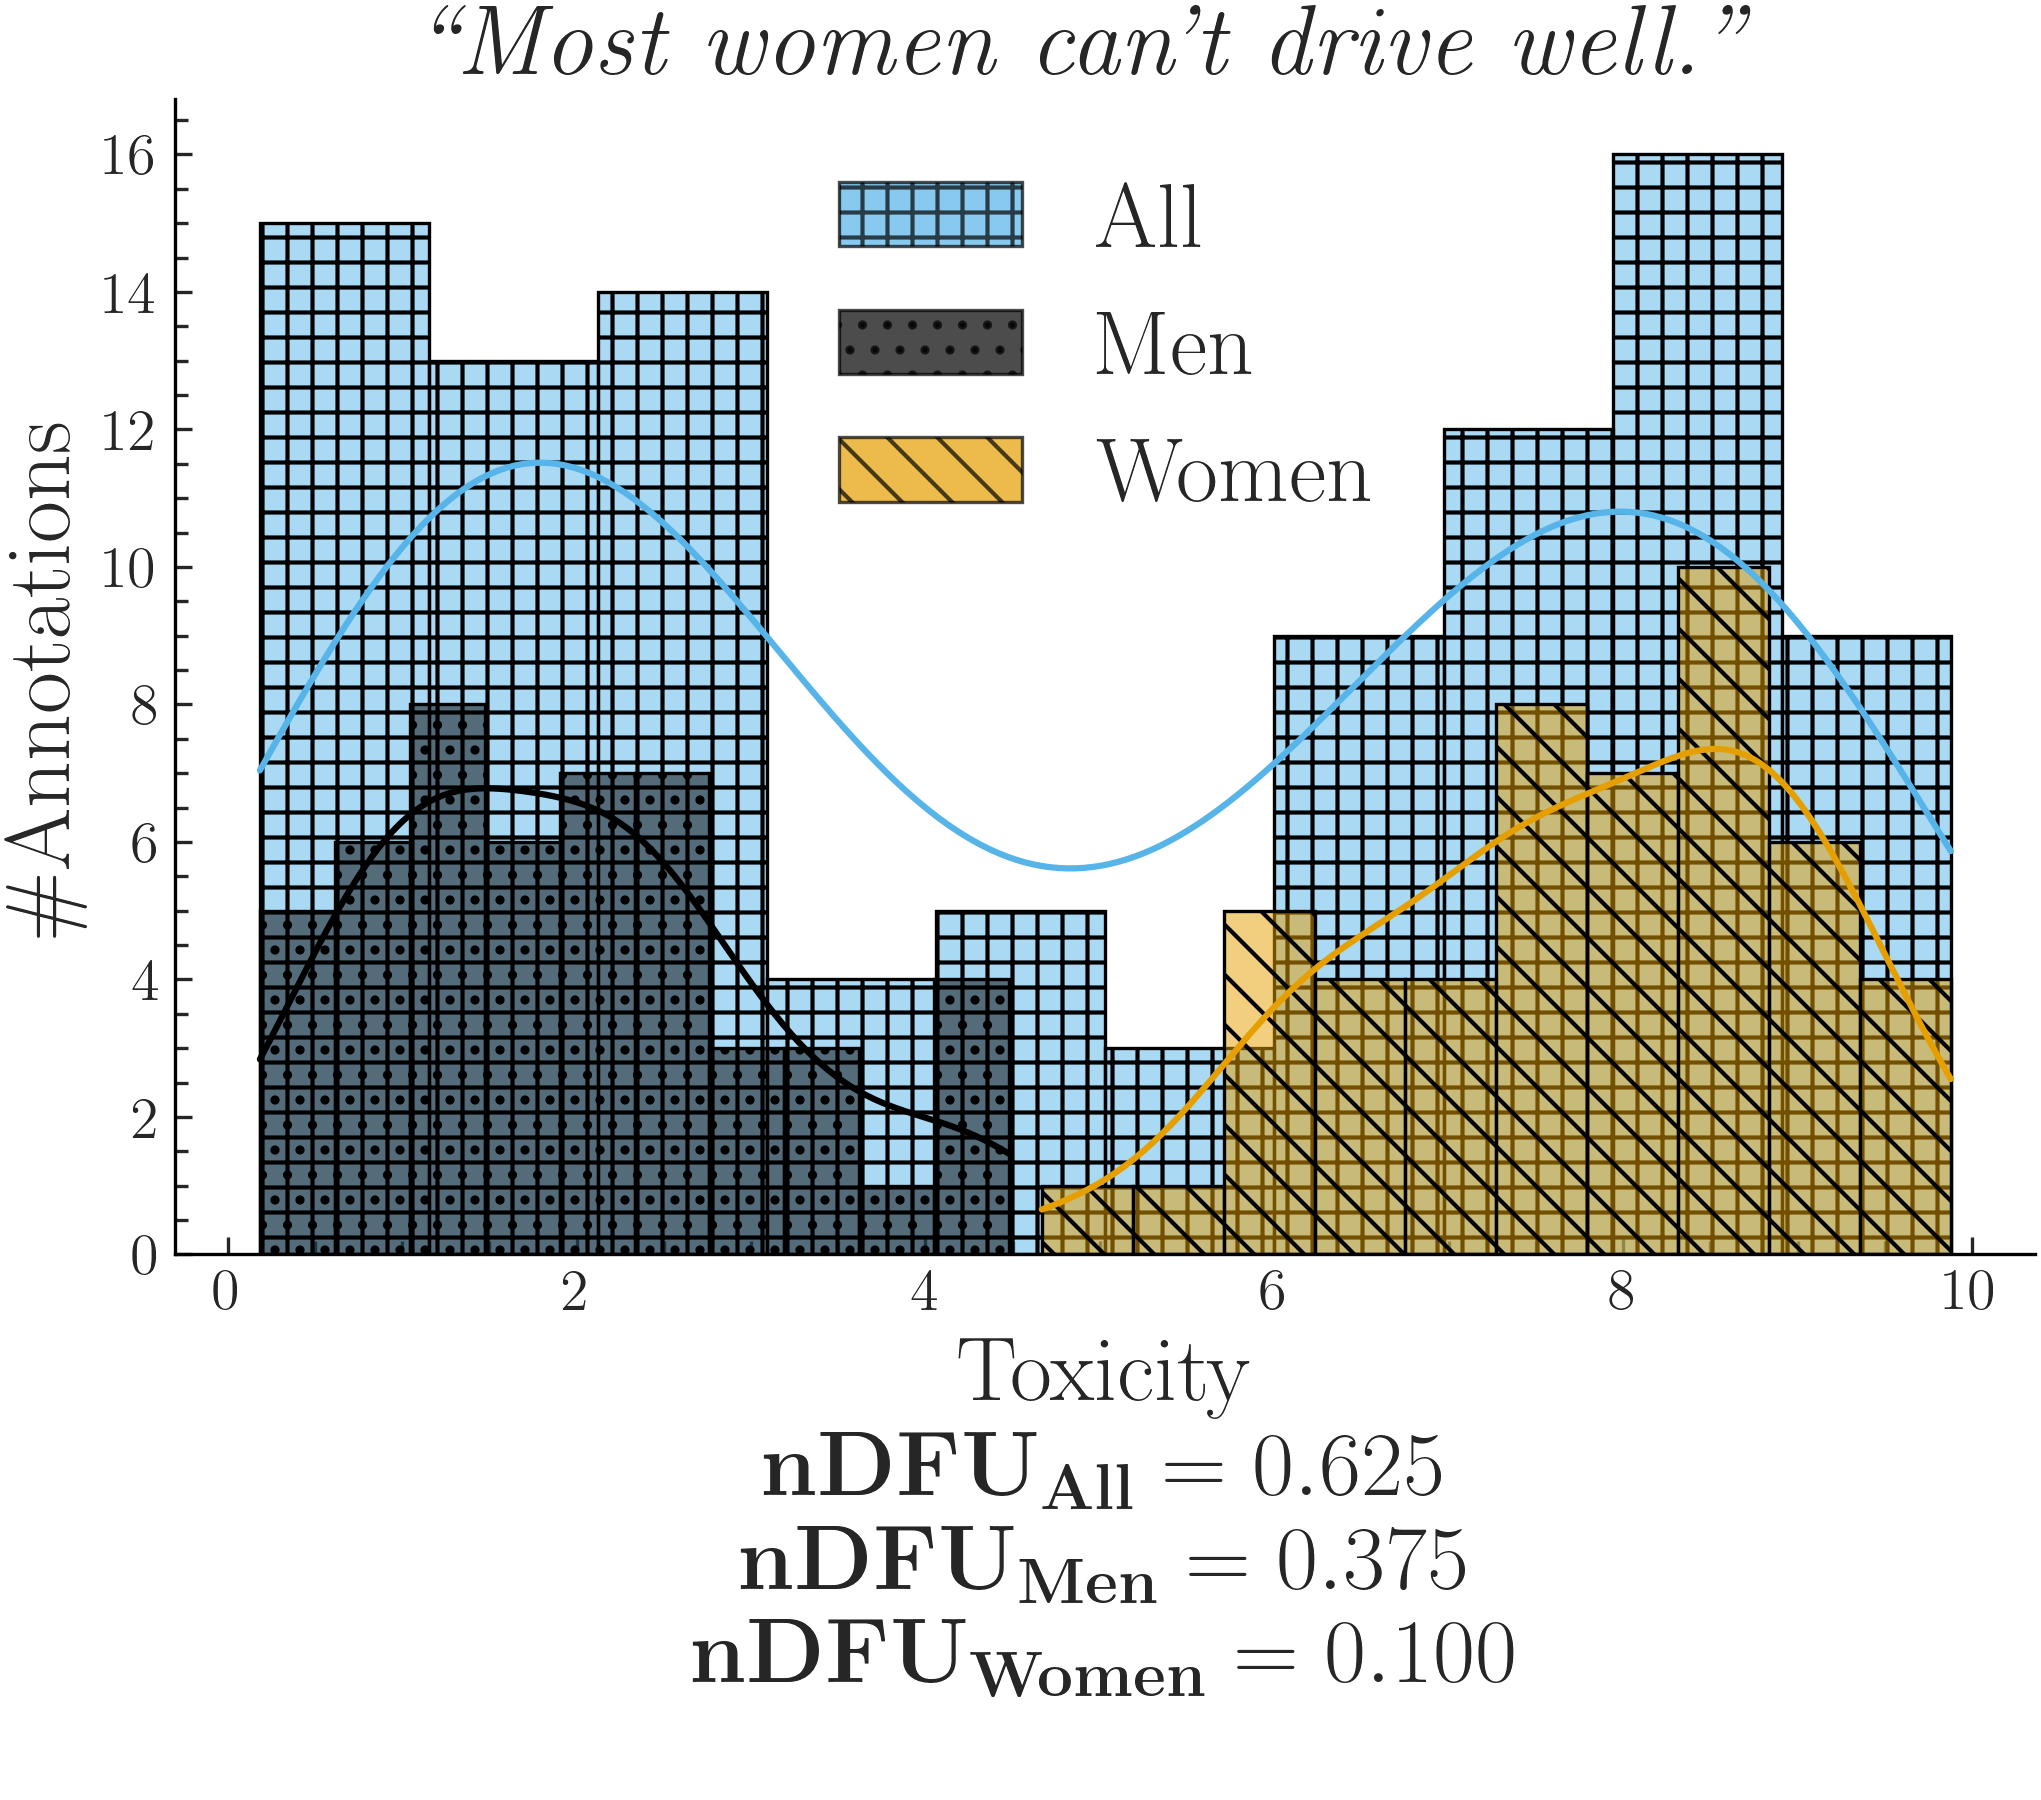
\includegraphics[width=0.55\textwidth]{ndfu_combined.png}
	\caption{Simulated experiment describing a polarizing comment where male and female annotators agree between themselves, but disagree with the opposite gender.}
	\label{fig:ndfu_combined}
\end{figure}

Intuitively, a group partially explains the polarization of a comment $c$ when the annotations of that group $A(c \given g) = \{a(c, g') \in A(c) \given g'=g\}$ exhibit higher polarization compared to the full set of annotations $A(c)$. Consider the case where a misogynistic comment is annotated for toxicity by male and female annotators shown in Fig.~\ref{fig:ndfu_combined}. The annotations are generally polarized ($nDFU_{all}=.62$); but both female ($nDFU_{women}=.10$) and male ($nDFU_{men}=.37$) annotators exhibit low polarization between their respective groups. This pattern suggests that the overall polarization is partially caused by substantive disagreements between male and female annotators.\footnote{\label{foot:iterative}Since polarization persists among male annotators, another subgroup of men may also contribute to it.}


\subsection{Inherent polarization}
\label{sec:inherent:inherent}

\subsubsection{What is it?}

\acf{ip} refers to disagreement that cannot be attributed to \emph{any specific} grouping of annotators; that is, polarization that exists no matter how we split the annotators in any arbitrary group. Prior work~\cite{pavlopoulos-likas-2024} attributed polarization to annotator groups only when the observed polarization for each individual group became exactly zero (e.g. $nDFU(all) > nDFU(men)=nDFU(women) = 0$). The presence of \ac{ip} would invalidate this theory, since there would be no possible group or combination of groups $g \textit{ s.t. } nDFU(g) = 0$.

\begin{definition}[Inherent Polarization]
	\label{def:inherent}
	Polarization that cannot be explained by any known or latent annotator grouping.
\end{definition}


Formally, the \ac{ip} for a single comment $c$ is the minimum polarization exhibited by any arbitrary group:
\begin{equation}
	\label{eq:inherent}
	Pol_{inh}(c) =
	\min_{S \subseteq A(c),\, |S| \ge 3}
	\left\{
	\textit{nDFU}(S)
	\right\}
\end{equation}

When considered exhaustively, these theoretical, random groups include both observed and latent groups (e.g., annotators may be less strict if they had lunch prior to annotation). Since \ac{ndfu} operates only when a group has at least three annotators (Eq.~\ref{eq:ndfu}), this yields $\sum_{k=3}^{n} \binom{n}{k}$ possible groups.


\subsubsection{Experimental setup}
\label{sec:inherent:experimental}

We systematically explore the space of annotator groups by generating random partitions for each comment. Since enumerating all subsets is computationally intractable for large annotator counts, we establish an upper bound via Monte Carlo sampling by drawing $k$ random partitions with random sizes:

\begin{equation}
	\label{eq:random}
	Pol_{inh}^{MC}(c) =
	\min_{j=1}^{k}
	\left\{
	\textit{nDFU}\!\left(\tilde{r}_j(A(c))\right)
	\right\}
\end{equation}
\noindent where $\tilde{r}$ is an operator that selects a randomly sized, randomly selected subset. Since Eq.~\ref{eq:random} considers a strict subset of Eq.~\ref{eq:inherent}, it provides an upper bound for it:  
\begin{equation}
	\label{eq:lower-bound}
	Pol_{inh}^{MC}(c) \ge Pol_{inh}(c) \forall c
\end{equation}


\subsubsection{Does it exist?}
\label{sec:inherent:results}

\begin{figure}[t]
	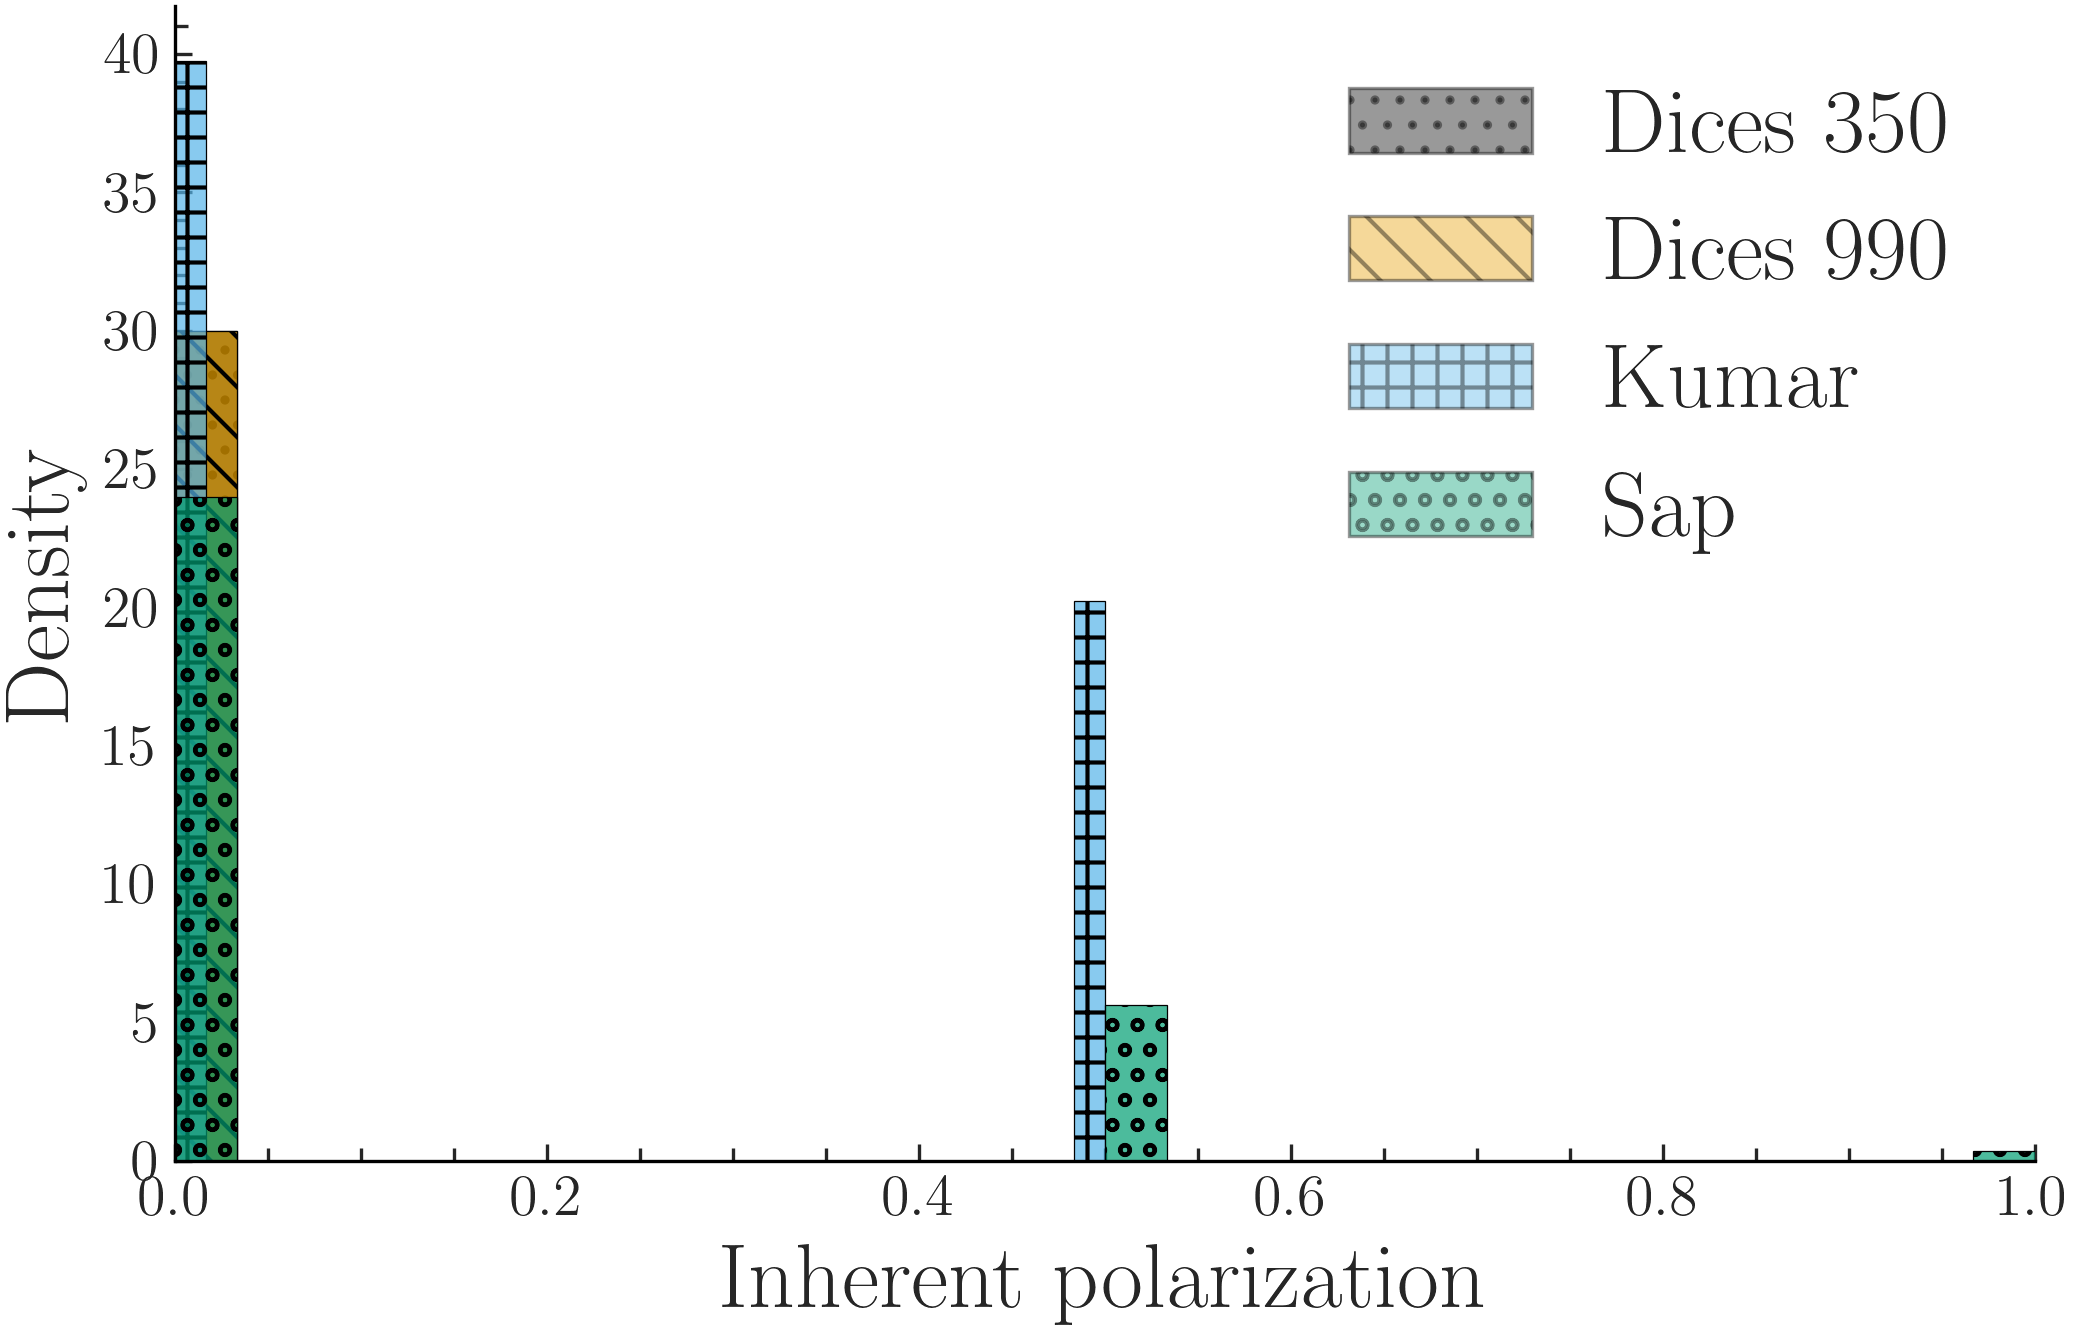
\includegraphics[width=0.55\textwidth]{apriori.png}
	\caption{\ac{ip} across our datasets (\S\ref{sec:datasets}). Contrary to assumptions made in prior work, \ac{ip} is commonly non-zero and can even reach $nDFU = 1$ in datasets with low annotator counts.}
	\label{fig:apriori}
\end{figure}

We compute the \ac{ip} for each comment across the four datasets. For Sap and Kumar, we use the exhaustive formulation (Eq.~\ref{eq:inherent}), whereas for the two DICES datasets we rely on the Monte Carlo approximation with $k=1000$ (Eq.~\ref{eq:random}). Fig.~\ref{fig:apriori} shows that in all DICES comments there exists at least one group that fully accounts for the observed polarization.\footnote{$Pol_{inh}^{MC}(c)=0 \Rightarrow Pol_{inh}(c)=0$ due to Eq.~\ref{eq:lower-bound}. The same logic applies if we tried to increase the number of random partitions in Eq.~\ref{eq:random}.} Interestingly, this observation does not hold for the Kumar and Sap datasets, despite evaluating all possible annotator groups exhaustively. See App.~\ref{app:inherent} for a qualitative look through comments with high InPol.

\begin{finding}
	\label{finding:inherent}
	Comments may exhibit a degree of \ac{ip} that cannot be attributed to any known or latent annotator grouping given the annotators present in the dataset.
\end{finding}


\subsubsection{Why does it exist?}
\label{sec:inherent:why}

\begin{hypothesis}[Low annotator count]
	\label{hyp:few-annotators}
	A low number of annotators per item may provide our model with insufficient information.
\end{hypothesis}

\begin{hypothesis}[Inaccessible groups]
	\label{hyp:groups}
	\ac{ip} may arise from the presence of partially represented groups within the annotator pool. While these groups are responsible for the observed polarization, they may go undetected in our current methodology if they are represented by only one or two annotators, as these groups are discarded (\S\ref{sec:inherent:inherent}). 
\end{hypothesis}

Both of these explanations are plausible and reflect known limitations of most \ac{nlp} datasets, although we lack such datasets with large annotator counts per item to provide a definitive answer. The DICES datasets can in principle be used for this purpose. However, even when repeating the experiment using random annotator subsets (ranging from 5 to 50 annotators) and taking the maximum across ten random samples for each subset size, \emph{we still observed zero \ac{ip}} (App.~\ref{app:ablation:dices}). This finding either invalidates both hypotheses, or indicates that the DICES datasets are structurally different. The latter explanation is plausible given that the annotation targets are LLM texts, which may be relatively unsubtle compared to human comments, as supported by low overall polarization (Fig.~\ref{fig:dataset-polarization}; App~\ref{app:ann_details}).


\subsection{Polarization is directional}
\label{sec:apunim:conflicting}

\begin{figure}[ht]
	\centering
	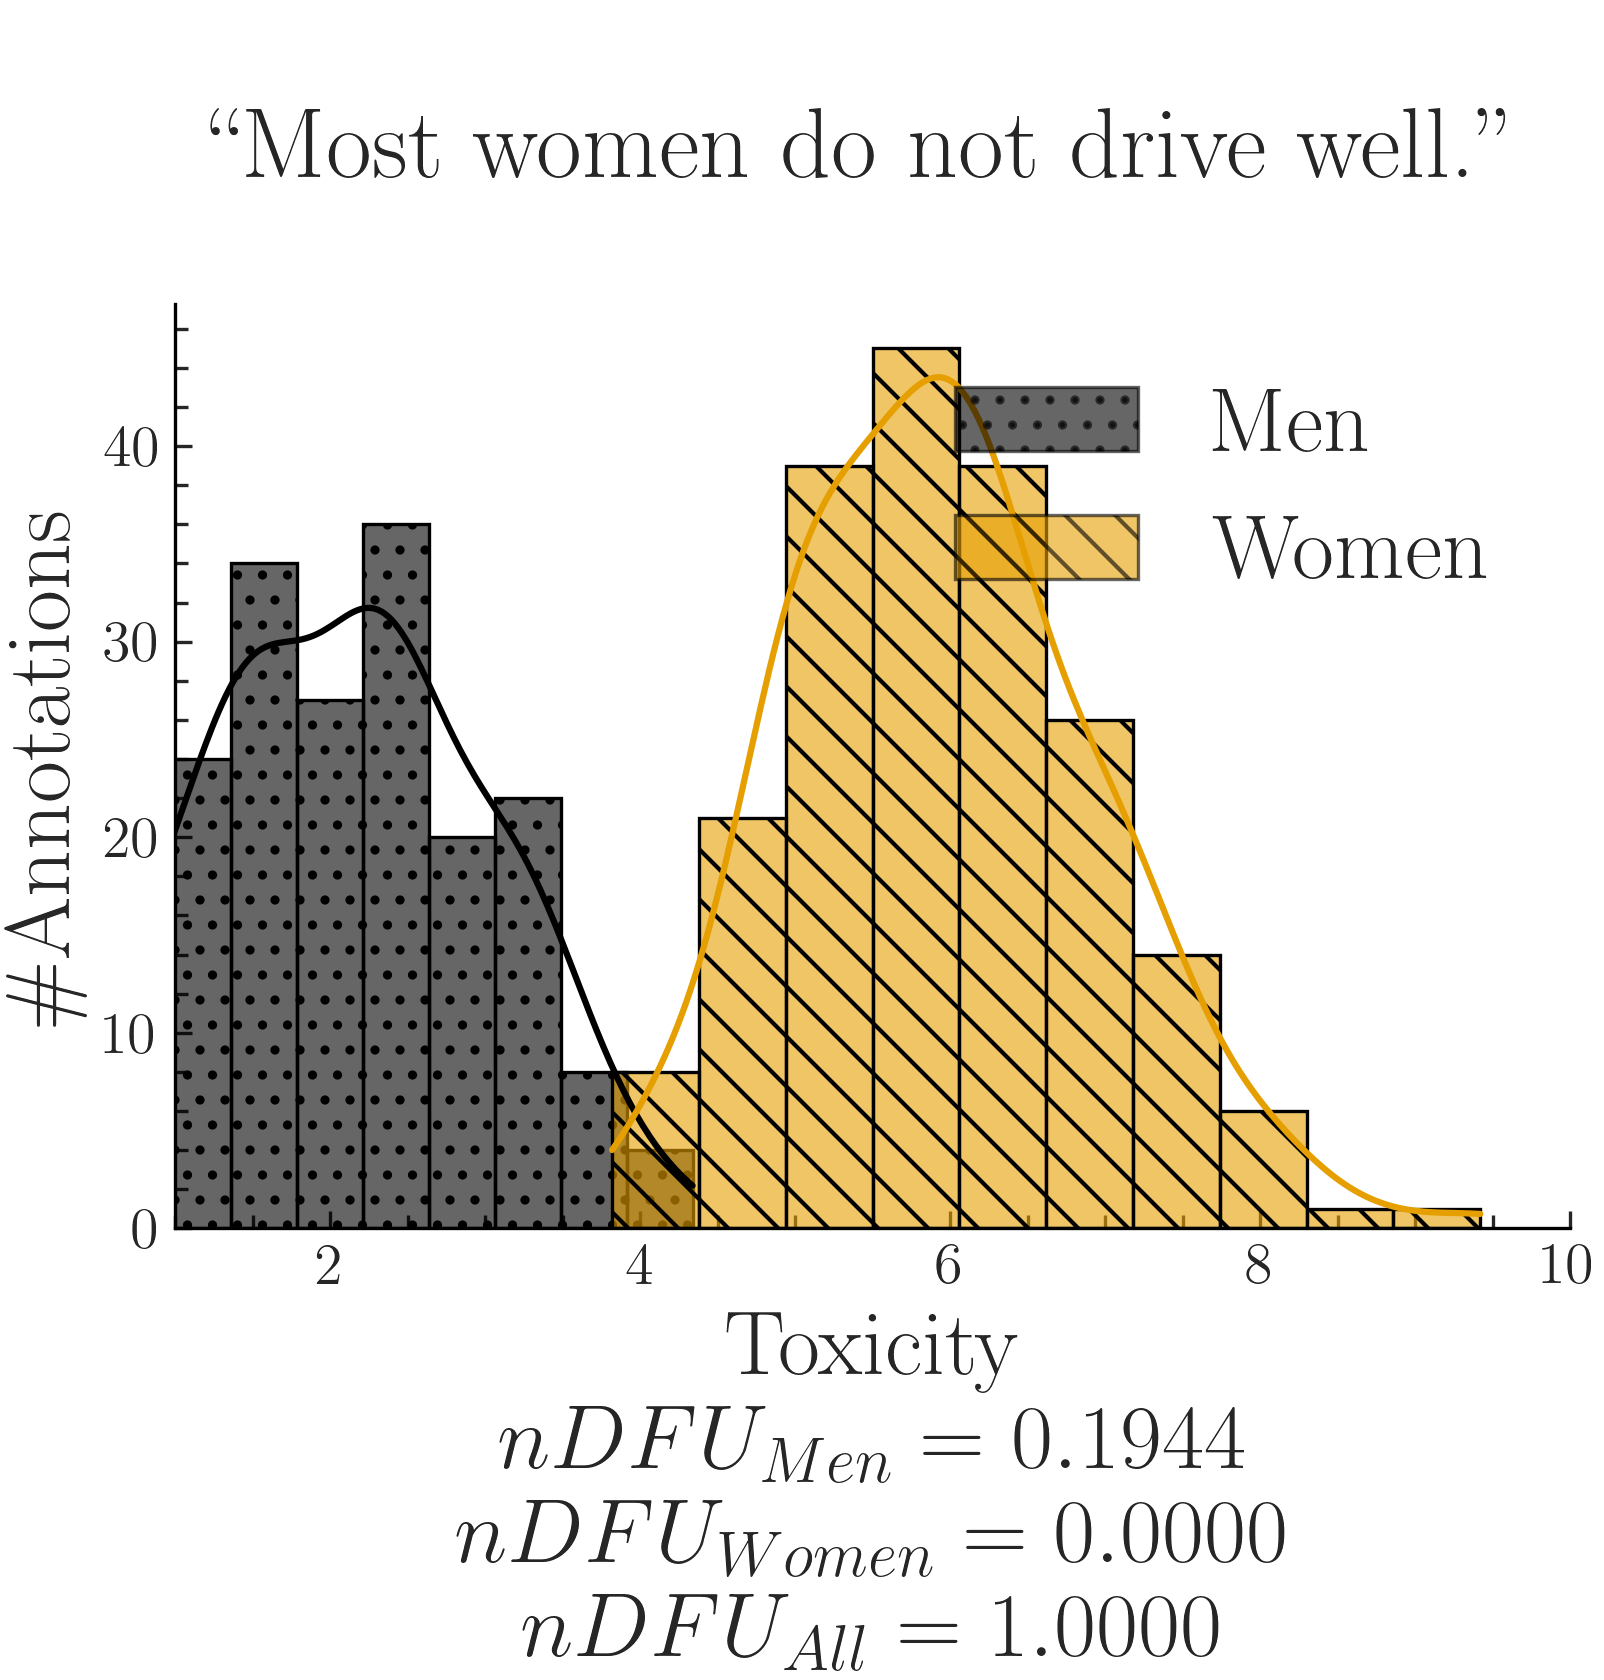
\includegraphics[width=0.32\linewidth]{ndfu_comment1.png}
	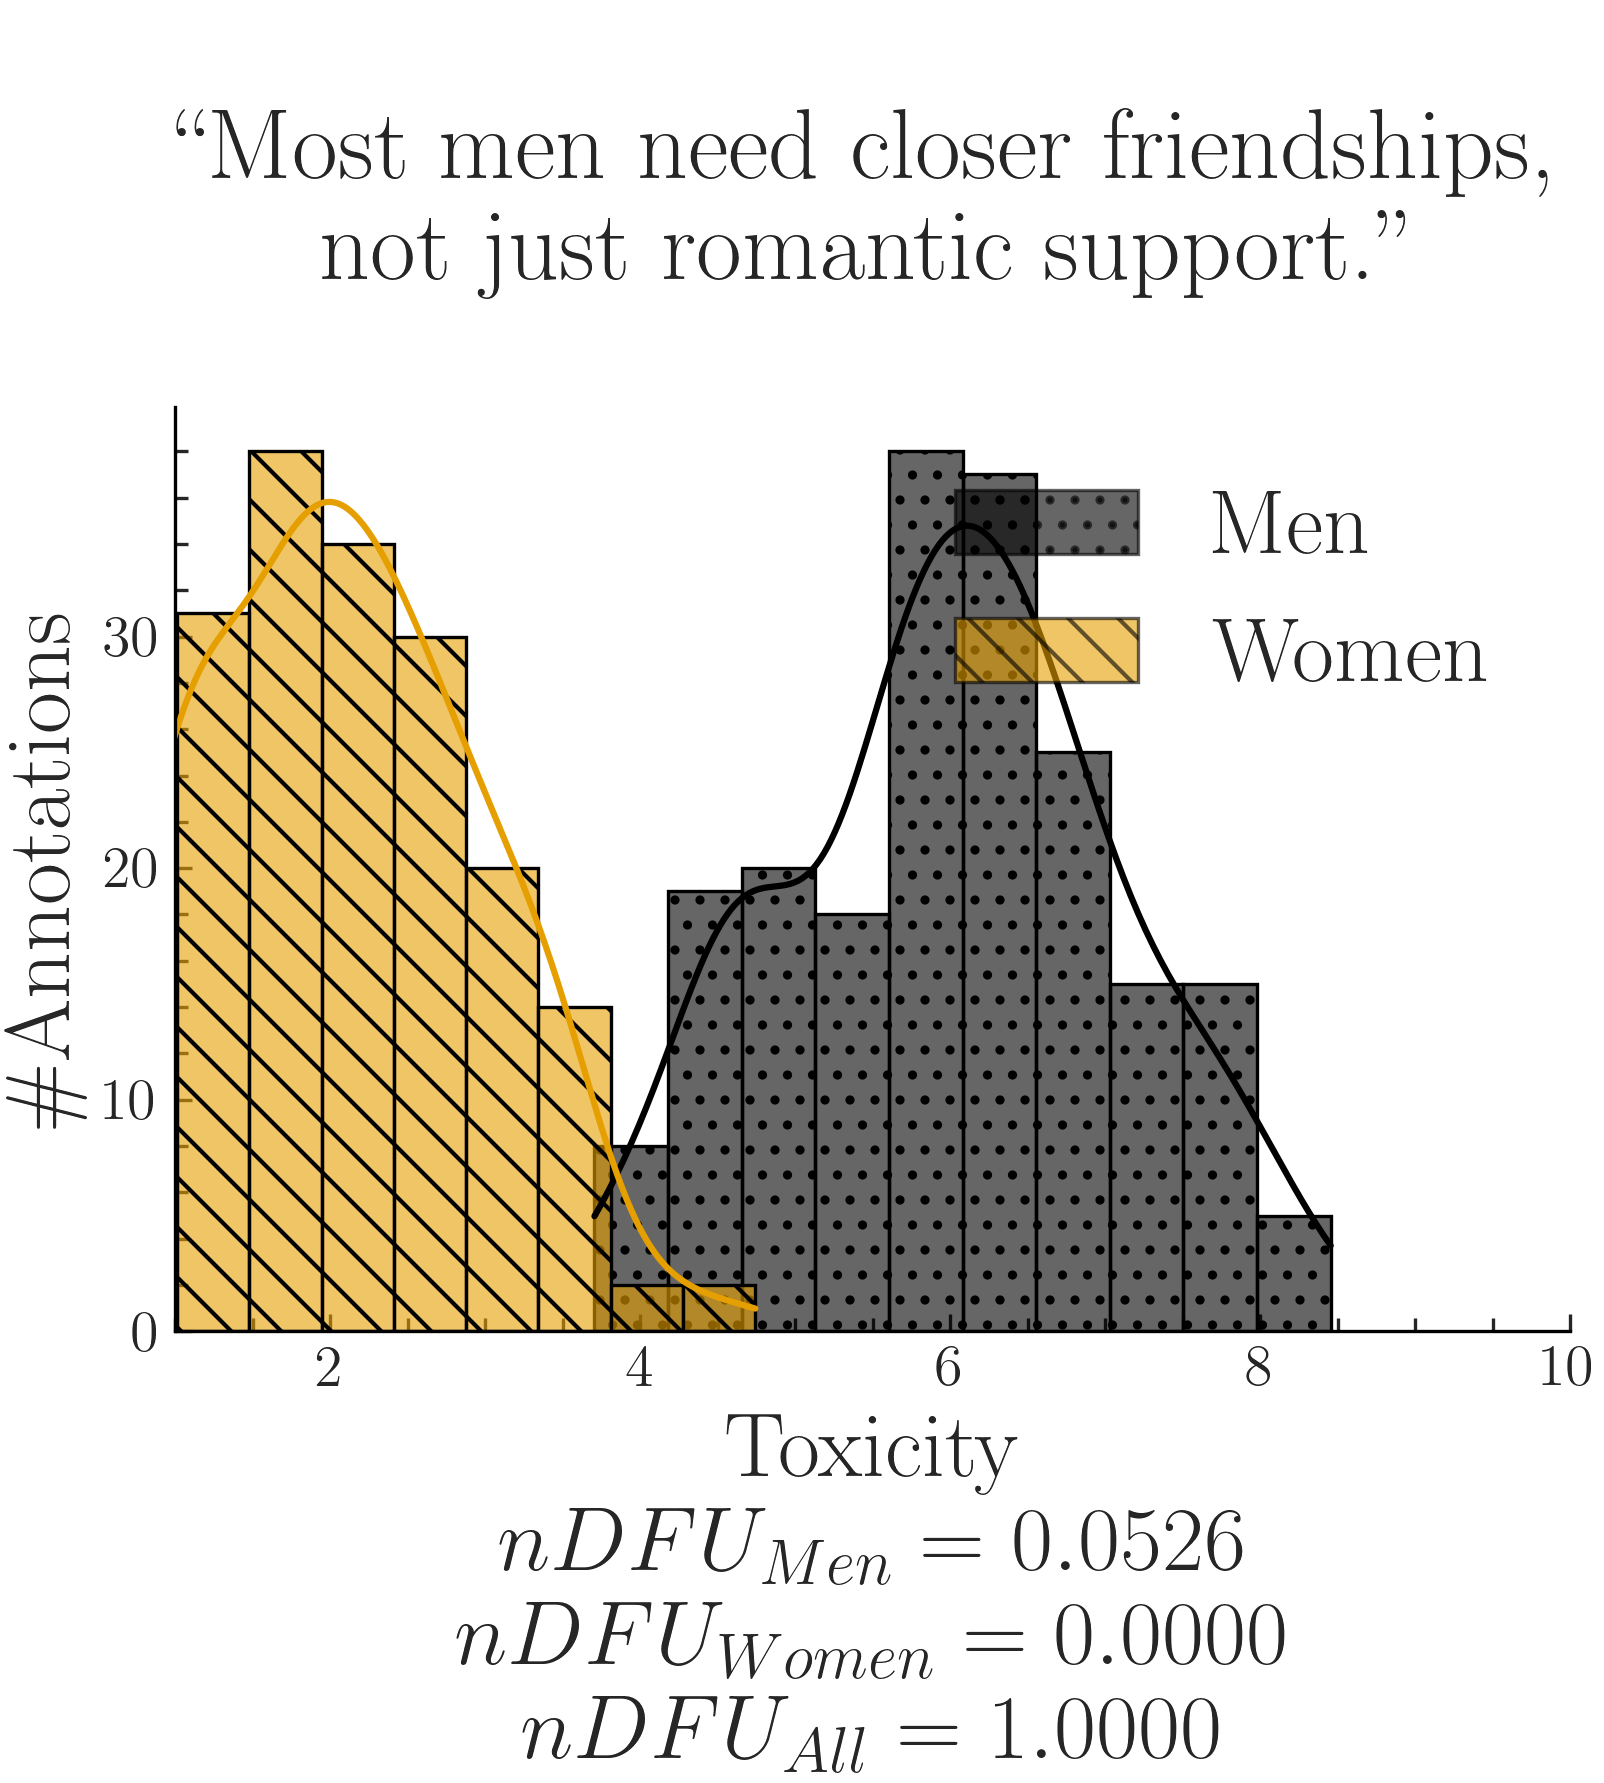
\includegraphics[width=0.32\linewidth]{ndfu_comment2.png}
	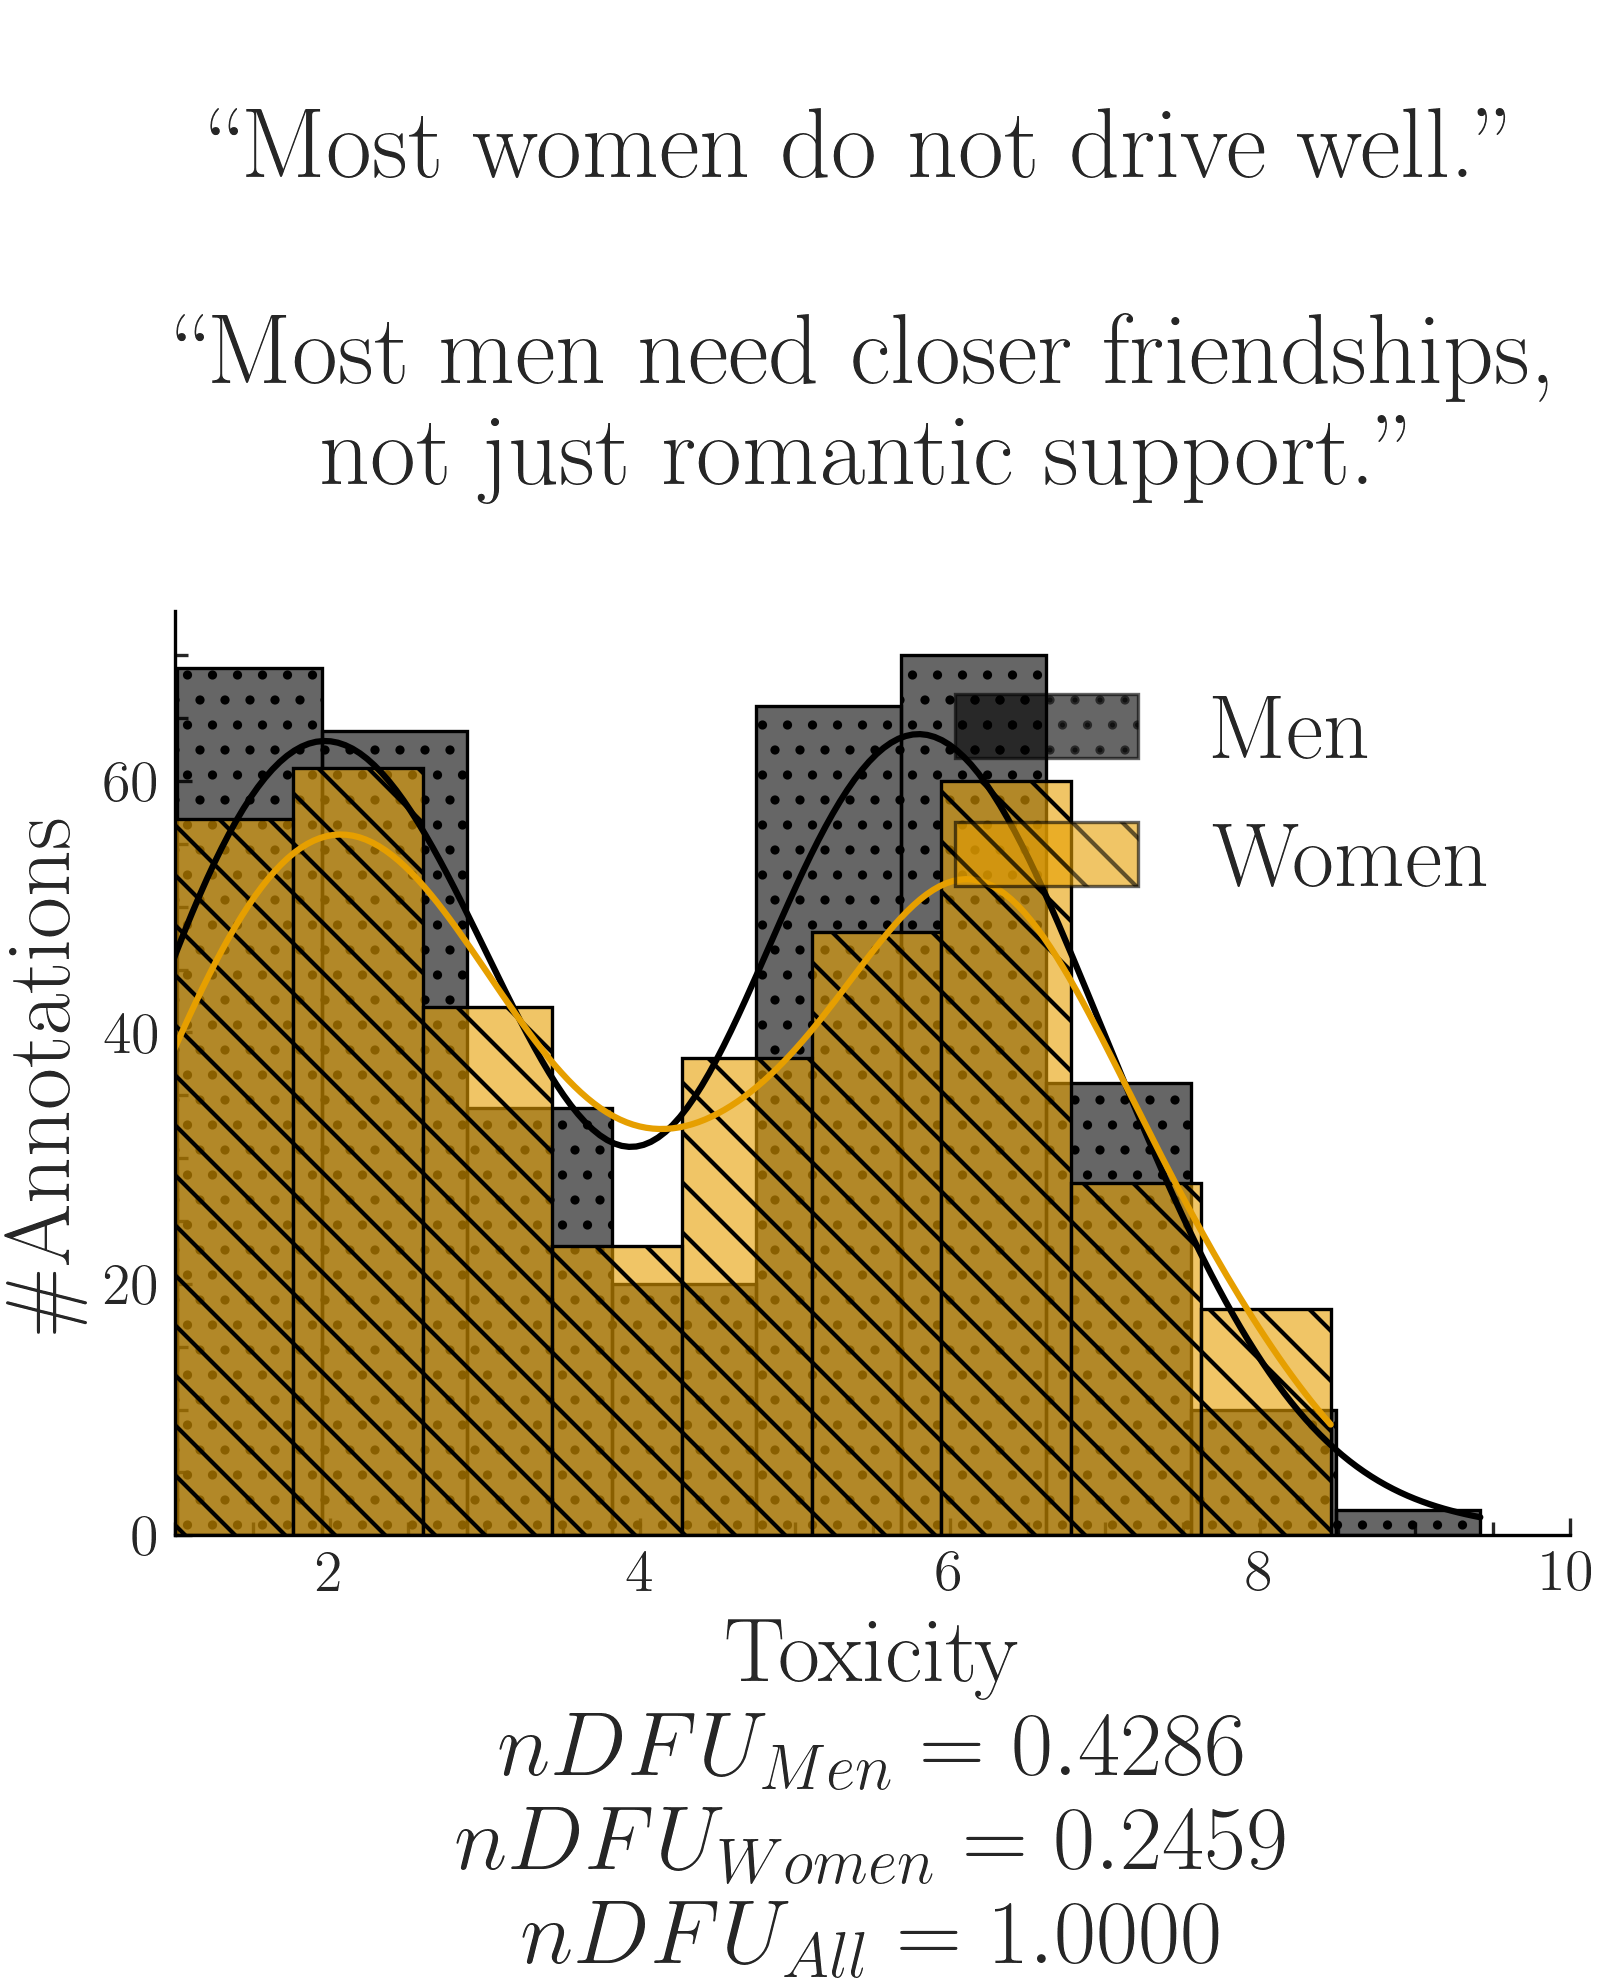
\includegraphics[width=0.32\linewidth]{ndfu_discussion.png}
	\caption{A synthetic experiment simulating a polarizing discussion with two comments where annotators disagree about which one is toxic. When we aggregate the comments, we unintentionally change the comparison: instead of comparing two unimodal distributions (each comment viewed separately) with two bimodal distributions (their aggregated annotations), we end up comparing two bimodal distributions, obscuring the source of the polarization (polarization explained by gender, but not shown).}
	\label{fig:ndfu_discussion}
\end{figure}

One way of potentially overcoming annotator sparsity, is aggregating annotations between comments. Fig.~\ref{fig:ndfu_discussion} shows an experiment where we combine annotations across two comments. We observe that, should the two comments be polarized for the opposite reason, the opposing polarization effects might balance each other out, leading to a false negative. Therefore, any statistics must be computed on the comment-level; annotations should never be aggregated across comments.\footnote{A similar assumption was followed in early parametric approaches, which assumed different parameters for each comment~\cite{checco_2017}.}

\begin{finding}
	\label{finding:conflicting}
	Polarization has a unique direction for each comment which may compromise cross-comment aggregation.
\end{finding}


\section{How do we attribute the rest?}
\label{sec:apunim}

\subsection{Apriori polarization}
\label{sec:apunim:group-vs-global}

Instead of using \ac{ip}, which represents the minimum possible polarization exhibited by any group, we calculate the \emph{expected} (average). Therefore, we do not test whether the group is polarized against the whole; nor whether the group explains \emph{some polarization} (as would be the case if we used Eq.~\ref{eq:inherent}), but rather whether the group explains polarization \emph{more than other groups}.

\begin{definition}[Apriori polarization]
	\label{def:apriori}
	The expected polarization of a comment's annotations.
\end{definition}

Specifically, we define apriori polarization for a comment $c$ as:
\begin{equation}
	\label{eq:apriori}
	Pol_{apr}(c) = \frac{1}{t} \sum_{i=1}^t  \textit{nDFU}(\tilde{r}_i (A(c)))
\end{equation}
\noindent where $\tilde{r}$ is the random partition operator (see Eq.~\ref{eq:inherent}). We explain why defining apriori polarization in this way is preferable to simpler alternatives in App.~\ref{app:stats:comparison}.


\subsection{Expanding to the whole dataset}
\label{sec:apunim:dataset}

We can estimate how much polarization is generally present in the dataset by simply averaging the \textit{apriori} polarization of its comments. Intuitively, a high apriori polarization score means that much of the polarization in the dataset is likely not driven by any single group.  
\begin{equation}
	\label{eq:apriori-dataset}
	Pol_{apr}(d) = \frac{1}{\lvert d \rvert} \sum_{c \in d} Pol_{apr}(c)
\end{equation}

We compare this quantity with the average observed polarization of all comments:
\begin{equation}
	\label{eq:observed}
	Pol_{obs}(d, g) = \frac{1}{\lvert d \rvert} \sum_{c \in d}  \textit{nDFU}(A(c \given g))
\end{equation}

We can now compare the polarization that is attributed to a single annotator group (Eq.~\ref{eq:observed}) to a prior one (Eq.~\ref{eq:apriori-dataset}). We define our normalized metric, \emph{apunim}, as:

\begin{equation}
	\label{eq:apunim}
	apunim(d, g) = \frac{Pol_{apr}(d) - Pol_{obs}(d, g)}{1 - Pol_{apr}(d)}
\end{equation}

\begin{definition}[Apunim]
	\label{def:apunim}
	The degree to which an annotator group contributes to overall polarization in a set of comments.
\end{definition}

\begin{itemize}
	\item$apunim(g) \approx 0$: The examined group does not meaningfully disagree with the other annotators.
	
	\item $apunim(g) > 0$: The examined group has fundamental disagreements with the other annotators. 
	
	\item $apunim(g) < 0$: The annotators of that group are polarized between themselves.
\end{itemize}


\subsection{Statistical significance}
\label{sec:apunim:statistical}

Since annotation histograms may be noisy, we additionally assess whether the observed apunim value could arise by chance. To assess statistical significance, we construct a null distribution of apunim values from the randomized partitions and compare the observed apunim against this distribution using a one-sample Student-\(t\) test. Thus, the null hypothesis states that the observed polarization is indistinguishable from polarization induced by random annotator assignments:

\begin{equation}
	\label{eq:pvalue}
	\begin{split}
		&H_0:\ 
		\bar{\textit{apunim}}_{\mathrm{rand}}(d,g)
		=
		\textit{apunim}(d,g) \\
		&H_a:\ 
		\bar{\textit{apunim}}_{\mathrm{rand}}(d,g)
		\neq
		\textit{apunim}(d,g)
	\end{split}
\end{equation}
\noindent where \(\bar{\textit{apunim}}_{\mathrm{rand}}(d,g)\) denotes the average apunim values obtained from $t$ randomized annotator partitions.

 We account for the presence of multiple subgroups in each \ac{pc} dimension using a multiple-hypothesis correction. For a detailed explanation of the p-value computation and the assumptions underlying the test, refer to App.~\ref{app:stats:pvalue}.


\section{Attributing real-life polarization to human groups}
\label{sec:results}

\subsection{Experimental setup}
\label{sec:results:experimental}

Assuming a confidence level of $\alpha=0.05$ we test whether any of the provided \ac{pc} dimensions can partially explain polarization in the annotations. Statistically significant results are presented in Table~\ref{tab:merged-apunim}. See App.~\ref{app:replication} for details on other parameters and execution times, and App.~\ref{app:full} for the full results.


\subsection{Which factors contribute to polarization?}
\label{ssec:results:factors}

\begin{table}[t]
	\small
	\centering
	\setlength{\tabcolsep}{4pt}
	\begin{minipage}[t]{0.485\textwidth}
		\begin{tabularx}{\linewidth}{X r r}
			\toprule
			\textbf{Group} & \textbf{Apunim} & \textbf{Support} \\
			\midrule
			\multicolumn{3}{c}{\textbf{DICES-350}} \\
			\midrule
			\rowcolor{gray!15}
			Ethnicity=Asian & -.066 & 8138 \\
			Education=Other & .021 & 2191 \\
			\midrule
			\multicolumn{3}{c}{\textbf{DICES-990}} \\
			\midrule
			\rowcolor{gray!15}
			Ethnicity=AfricanAm & -.091 & 5810 \\
			\rowcolor{gray!15}
			Ethnicity=Latino & .133 & 6610 \\
			\rowcolor{gray!15}
			Ethnicity=Other & -.074 & 24321 \\
			\rowcolor{gray!15}
			Ethnicity=White & .120 & 11392 \\
			Age=GenZ & -.063 & 13741 \\
			Age=GenX+ & .046 & 14384 \\
			Education=High school & -.075 & 7419 \\
			\rowcolor{gray!15}
			Gender=Man & -.027 & 32494 \\
			\rowcolor{gray!15}
			Gender=Woman & .024 & 33471 \\
			\midrule
			\multicolumn{3}{c}{\textbf{Sap}} \\
			\midrule
			\rowcolor{gray!15}
			Ethnicity=AfricanAm & .042 & 4 \\
			\rowcolor{gray!15}
			Gender=Man & -.091 & 1439 \\
			\rowcolor{gray!15}
			Gender=Woman & .244 & 877 \\
			\bottomrule
		\end{tabularx}
	\end{minipage}
	\hfill
	\begin{minipage}[t]{0.485\textwidth}
		\begin{tabularx}{\linewidth}{X r r}
			\toprule
			\textbf{Group} & \textbf{Apunim} & \textbf{Support} \\
			\midrule
			\multicolumn{3}{c}{\textbf{Kumar}} \\
			\midrule
			\multicolumn{3}{c}{A. Innate Characteristics} \\
			\midrule
			\rowcolor{gray!15}
			Ethnicity=White & -.029 & 6619 \\
			Education=College & -.034 & 2508 \\
			SexOrient=Heterosexual & -.050 & 5721 \\
			\rowcolor{gray!15}
			IsTrans=No & -.079 & 1697 \\
			\midrule
			\multicolumn{3}{c}{B. Experiences and Ideologies} \\
			\midrule
			HasBeenTargeted=False & -.048 & 6632 \\
			IsParent=No & -.069 & 5514 \\
			IsParent=Yes & .049 & 6216 \\
			ReligionImportant=No & -.062 & 3864 \\
			ReligionImportant=Very & .052 & 4062 \\
			SeenToxicity=False & .035 & 3050 \\
			SeenToxicity=True & -.077 & 6360 \\
			\bottomrule
		\end{tabularx}
	\end{minipage}
	\caption{Statistically significant ($p<0.05$) apunim results across the four datasets. Gray rows show \texttt{Ethnicity} and \texttt{Gender} groups. ``Support'' refers to number of annotations. Consult App.~\ref{app:full} for the full results.}
	\label{tab:merged-apunim}
\end{table}

\paragraph{Ethnicity} Polarization is consistently attributed to ethnicity across all datasets, confirming prior work suggesting that it is a systematic source of annotator disagreement in these tasks~\cite{goyal2022your}. We note that polarization attribution does not have a consistent direction across datasets, which we believe to be caused by studies using different ethnic subgroups, allowing polarization detection on the level of \acp{pc}, but distorting subgroup attribution.

\paragraph{Gender} In both DICES-990 and Sap, women are a consistent source of polarization (positive values), while men disagree among themselves (negative values). These results are consistent with previous findings regarding \ac{hs}~\citep{wojatzki2018women} and toxicity annotation~\cite{binns2017like}. Non-\emph{transgender} annotators also showed the highest degree of polarization in the Kumar dataset in absolute terms ($-.788$) suggesting that transgender annotators are a systematic source of annotator disagreement, although only the inverse effect is detectable due to annotator sparsity (hence the negative sign).

\begin{finding}
	\label{finding:categorical}
	Annotator ethnicity and gender are consistent causes of polarization.
\end{finding}

\begin{figure}[t]
	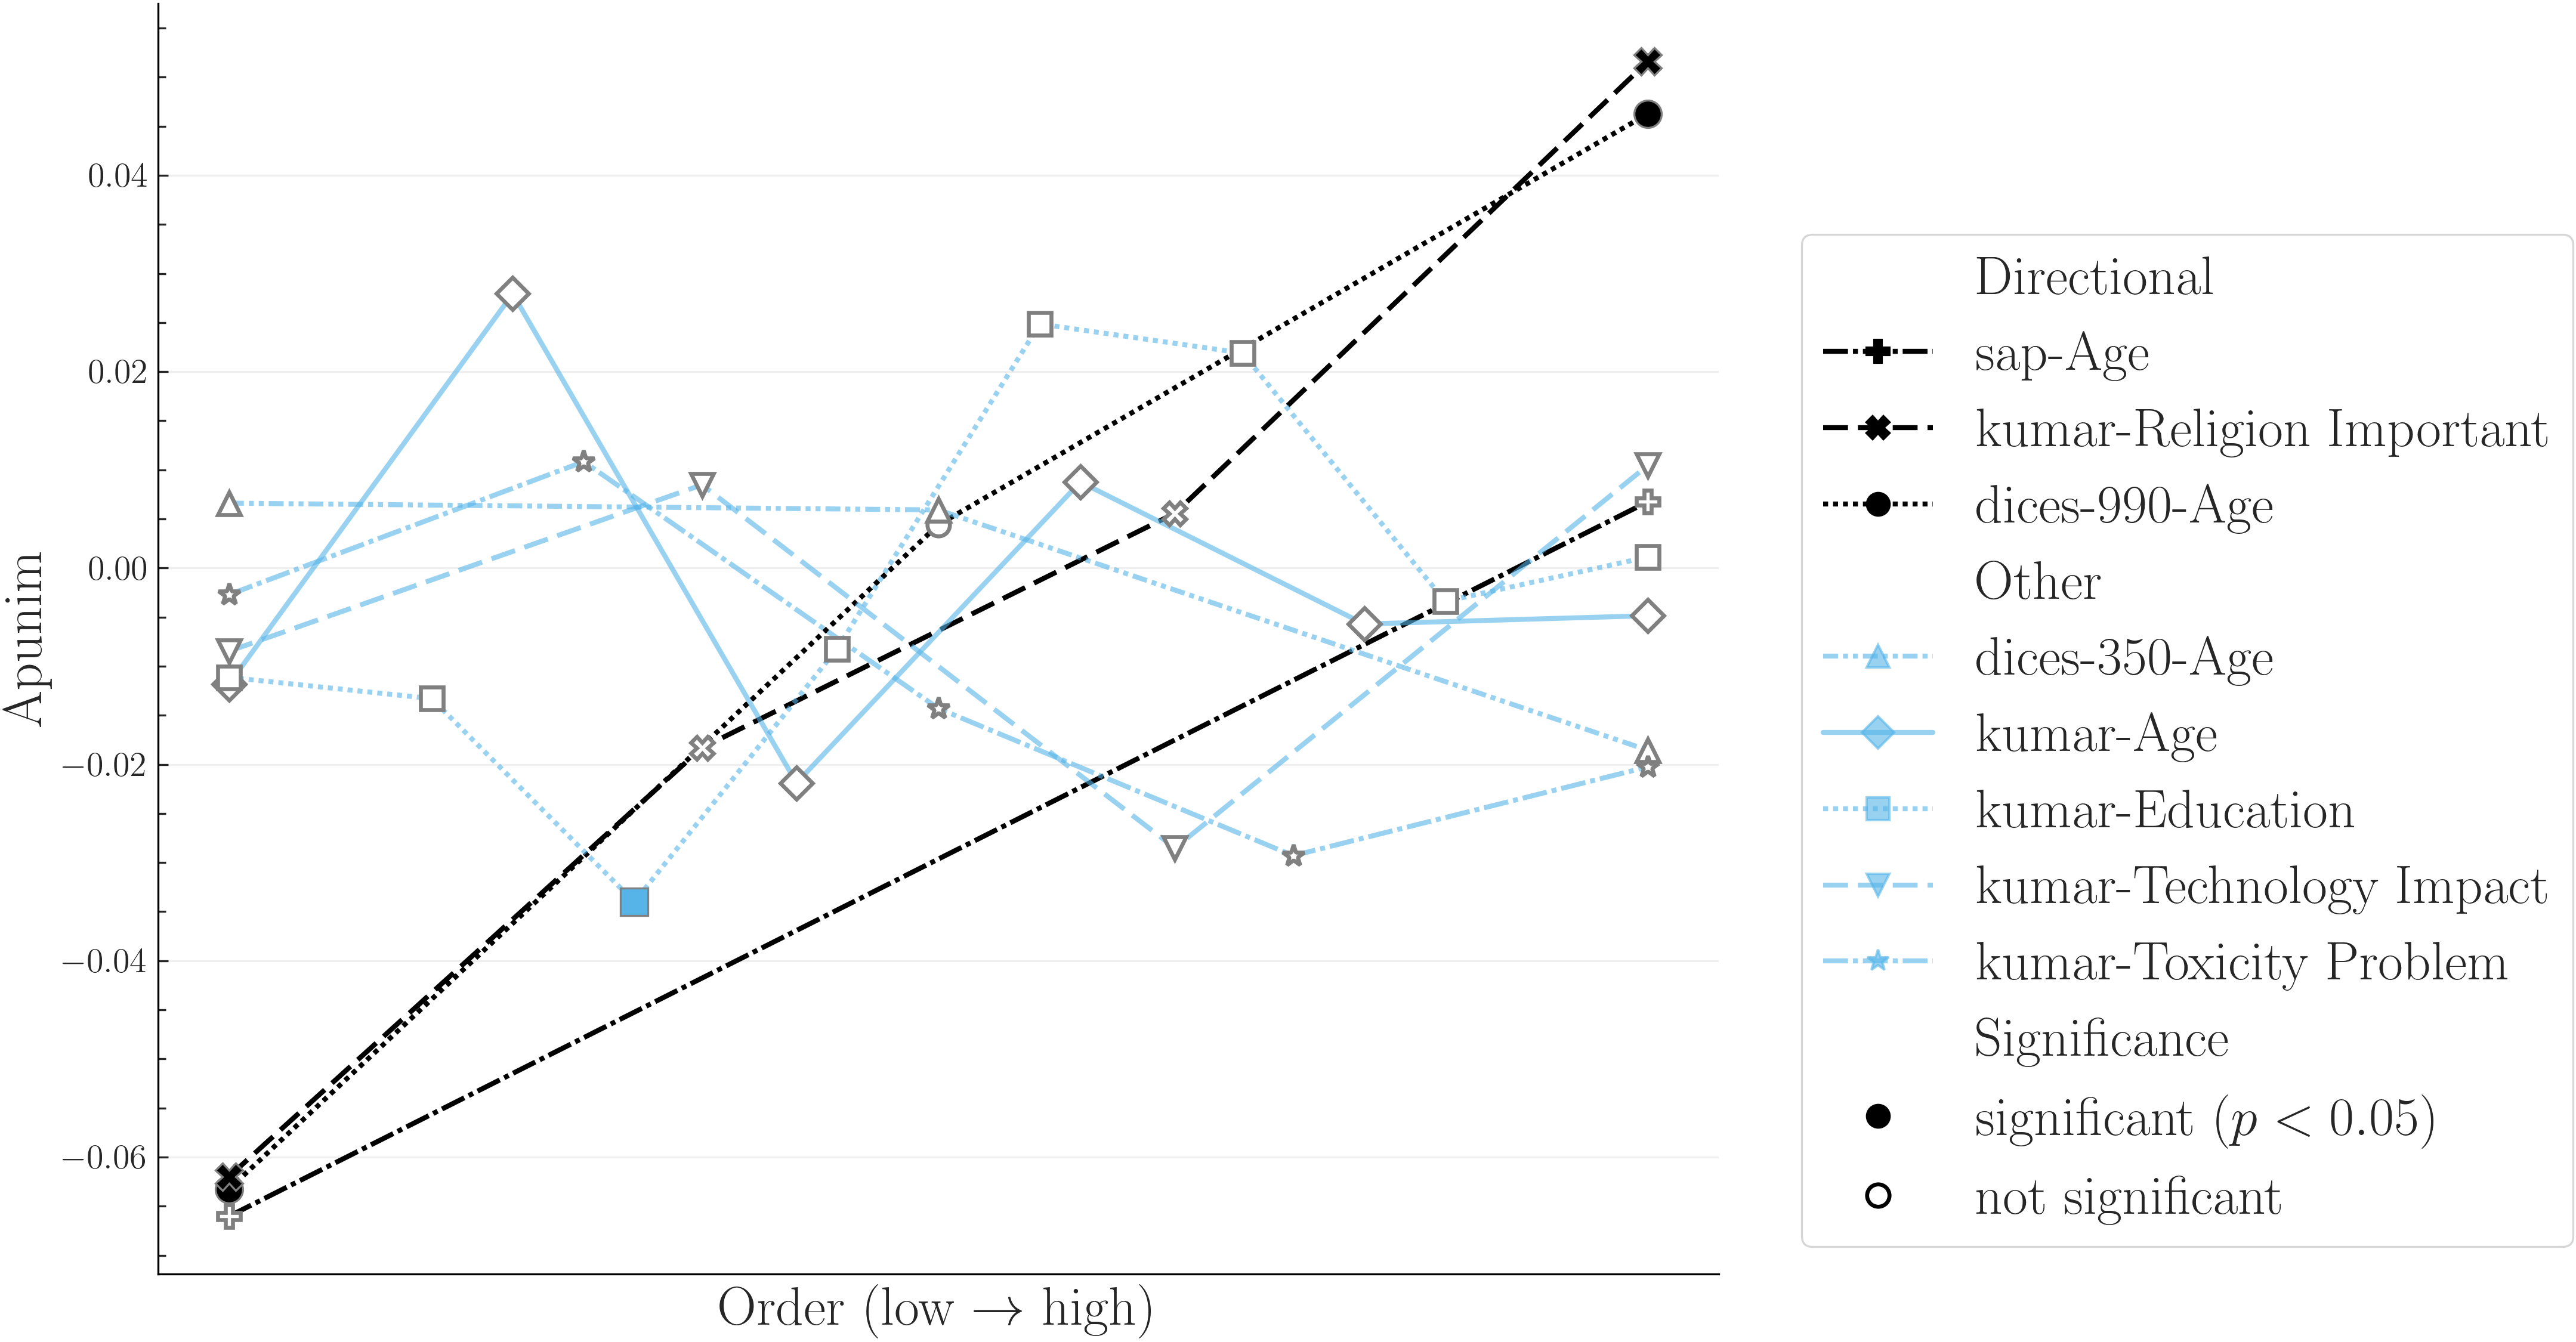
\includegraphics[width=0.6\textwidth]{apunim_ordinal.png}
	\caption{Polarization attribution trends in ordinal groups. The left side of the x-axis refers to young annotators, low education, low religiousness, and negativity towards the impacts of toxicity and technology. The full ordinal modes for each dimension and their individual labels can be found in App.~\ref{app:full}. We exclude groups with $<50$ annotations, since they near-universally result in zero apunim values due to lack of data.}
	\label{fig:ordinal}
\end{figure}

\paragraph{Ideology and experiences}  appear to be a more consistent source of annotator disagreement than inherent characteristics. Specifically, the Kumar dataset, which tracks ideological attributes, shows polarization attribution linked primarily to personal experiences and beliefs, rather than to sociodemographic dimensions, although further datasets are required to generalize this finding. The divide between ideology/personal experiences and innate sociodemographic characteristics has not been adequately explored in current literature and should be further studied in future work.

\paragraph{Religion} demonstrates a clear relationship with polarization attribution. According to Fig.~\ref{fig:ordinal}, highly devout annotators exhibit higher levels of self-agreement compared with other annotators (positive apunim). Non-religious annotators show a pattern of increased internal disagreement (negative apunim). Notably, this trend of internal disagreement gradually reverses as religious devoutness increases (increasing apunim).\footnote{The statistical insignificance observed during the transition from irreligious to highly religious groups may represent genuine shifts rather than inconclusive results, since Eq.~\ref{eq:pvalue} checks whether $apunim \neq 0$, given that $\bar{\textit{apunim}}_{\mathrm{rand}}(d,g)$  will usually be close to zero. This phenomenon may also apply to other ordinal \acp{pc}, such as \texttt{Age} in both Sap and DICES-990, but finer-grained subgroups are needed to verify this.}

\begin{finding}
	\label{finding:ideology}
	Pol. attribution may be more pronounced in ideological attributes and personal experiences. It also escalates as annotators become more religious.
\end{finding}


\section{Conclusion}
\label{sec:conclusion}

We investigated to what extent polarization can be attributed to annotator groups. We discovered as of yet unknown issues regarding the presence of inherent and conflicting polarization, which we treat using a new metric, \textit{apunim}. By applying this metric to four subjective \ac{nlp} datasets, we discover that (1) ethnicity and gender seem to generally drive polarization attribution, and (2) ideological groups may be more important than reported in the literature. Finally, we empirically investigate and discuss how our methodology interacts with (generally small in both annotations and size) current subjective \ac{nlp} datasets (App.~\ref{sec:ideal-dataset}) and release a PyPi library implementation to support further work.

%While we study one group at a time, we can instead turn to iteratively exploring polarized subgroups in future work, allowing us to gradually piece together a multidimensional explanation of polarization (see Footnote~\ref{foot:iterative},~\S\ref{sec:inherent:formulation}). It would also be interesting to explore to what extent LLM-as-a-judge systems reproduce the polarization patterns observed among different minority groups---which would solve the issues with annotation counts presented in our study.


\section*{Limitations}

\paragraph{Data limitations} Researchers often release only aggregated single-label annotations or omit annotator \ac{pc} characteristics entirely. As a result, both our analysis and the applicability of our framework are limited by the scarcity of suitable datasets. In addition, because datasets with large numbers of annotators per item are rare, our approach operates only at the dataset level. This limitation prevents us from identifying individual comments or examples that could serve as concrete explanations for the observed \textit{apunim} values.

\paragraph{Scope} It must be noted that the datasets utilized in this study are restricted to posts written in English and pertain exclusively to the Western, specifically U.S., cultural context. Consequently, the findings and observed phenomena are not necessarily generalizable to linguistic or cultural contexts outside of this scope, such as non-English languages or other global cultural spheres.

\paragraph{Confounding variables} Our analysis does not take into account confounding variables. It is plausible that some annotator groups are correlated with others (e.g., LGBTQ+ annotators may not lean into Conservatism). This is left for future work, as the scope of this analysis is deemed too large for this paper. Additionally, many datasets do not report anonymized IDs for the annotators, but only the annotations themselves, making this kind of analysis impossible. We leave our analysis as proof that our methodology can be used to surface polarization patterns, although future methods should allow for intergroup attribution.

\paragraph{Computational limitations} Additionally, our metric features some important practical limitations. It is computationally expensive when applied to very large datasets with a very large amount of \ac{pc} dimensions each featuring multiple distinct subgroups (App.~\ref{app:replication}). It also tends to underestimate polarization attribution when applied to many tens of thousands of items (App.~\ref{app:ablation}). Furthermore, the p-value estimates may falsely give the impression that zero-attribution effects are genuine, which should be taken into account when interpreting results. These limitations do not render our method insufficient---the first two issues can be solved by subsampling. We nevertheless believe that \ac{nlp} datasets should generally move away from huge annotated corpora, and instead towards smaller datasets with large annotator groups per item that sufficiently represent social subgroups.

\paragraph{Comparisons with other methods} Finally, although we compare findings across datasets and relate them to prior work, we do not directly compare polarization and agreement metrics, since they rely on fundamentally different assumptions and mechanisms (see \S\ref{sec:related:polarization}). These differences also make it difficult to fully explain certain patterns in our results, such as why some groups show statistically significant effects while others do not.


\section*{Ethics Statement}

\paragraph{Dual use concerns}The primary objective of this study is to identify systemic sources of polarization in subjective NLP datasets to facilitate the construction of more robust and equitable AI systems. However, given that our methodology allows for the quantitative attribution of specific judgment patterns to sociodemographic and ideological characteristics, we acknowledge three primary risks inherent in this research.

First, \emph{Discriminatory Profiling}: If the metric is applied outside of a dataset quality analysis, its ability to correlate specific judgment patterns with annotator groups could be misused for surveillance or unjust profiling. Second, \emph{Automated Bias Amplification}: The diagnostic patterns of polarization we detect are reflections of human systemic biases. Without human oversight, training subsequent models on these patterns risks automating and entrenching existing societal prejudices. Finally, the knowledge provided by \emph{apunim} could be \emph{weaponized}, allowing malicious actors to strategically target weak points in moderation systems or intentionally maximize societal conflict.

We stress that our metric functions strictly as a diagnostic warning signal. Any deployment in a real-world system must mandate a rigorous human-in-the-loop review, ensuring that identified patterns lead to systemic improvements (e.g., policy reform, demographic diversity initiatives) rather than merely justifying an automated system.

\paragraph{Data sourcing and privacy} All datasets employed in this study were either publicly accessible or provided to us by the original authors with full disclosure regarding the purpose of our research. No identifiable, personal information was included in our pipeline. We do not release proprietary data provided by the authors.

\paragraph{Examples used} Our study utilizes examples of comments that may be considered divisive across certain demographics. These examples were generated by our team solely for demonstration purposes. We explicitly state that the contents of these examples and the groups studied do not necessarily reflect the views or behaviors of the groups they represent, nor do they reflect the opinions of the authors.

\paragraph{Tools used} We used small, open-source LLMs (primarily a local Gemma-4 model) to perform minor stylistic adjustments throughout this document. Furthermore, we utilized open-source and proprietary models to generate portions of the code for the plots and experiments presented. All such AI-generated outputs have been meticulously checked and validated by the authors. 

\section*{Reproducibility Statement}
All code, data-processing scripts and the library implementing \emph{apunim} are released anonymously: library \librarylink, documentation \doclink, replication code \explink. Statistical procedures are detailed in App.~\ref{app:stats}, replication details (seeds, compute) in App.~\ref{app:replication}.

\bibliographystyle{iclr2026_conference}
\bibliography{refs}
\appendix


\section {Acronyms}

\begin{acronym}[WWW]
	\acro{ip}[InPol]{Inherent Polarization}
	\acro{ndfu}[nDFU]{normalized Distance From Unimodality}
	\acro{nlp}[NLP]{Natural Language Processing}
	\acro{gpl}[GPLv3]{GNU General Public Licence v3}
	\acro{aa}[AA]{African American}
	\acro{pc}[PC]{Personal Characteristic}
	\acro{hs}[HS]{Hate Speech}
	\acro{sd}[SD]{Standard Deviation}
\end{acronym}


\section{Annotation details}
\label{app:ann_details}

\begin{figure}[t]
	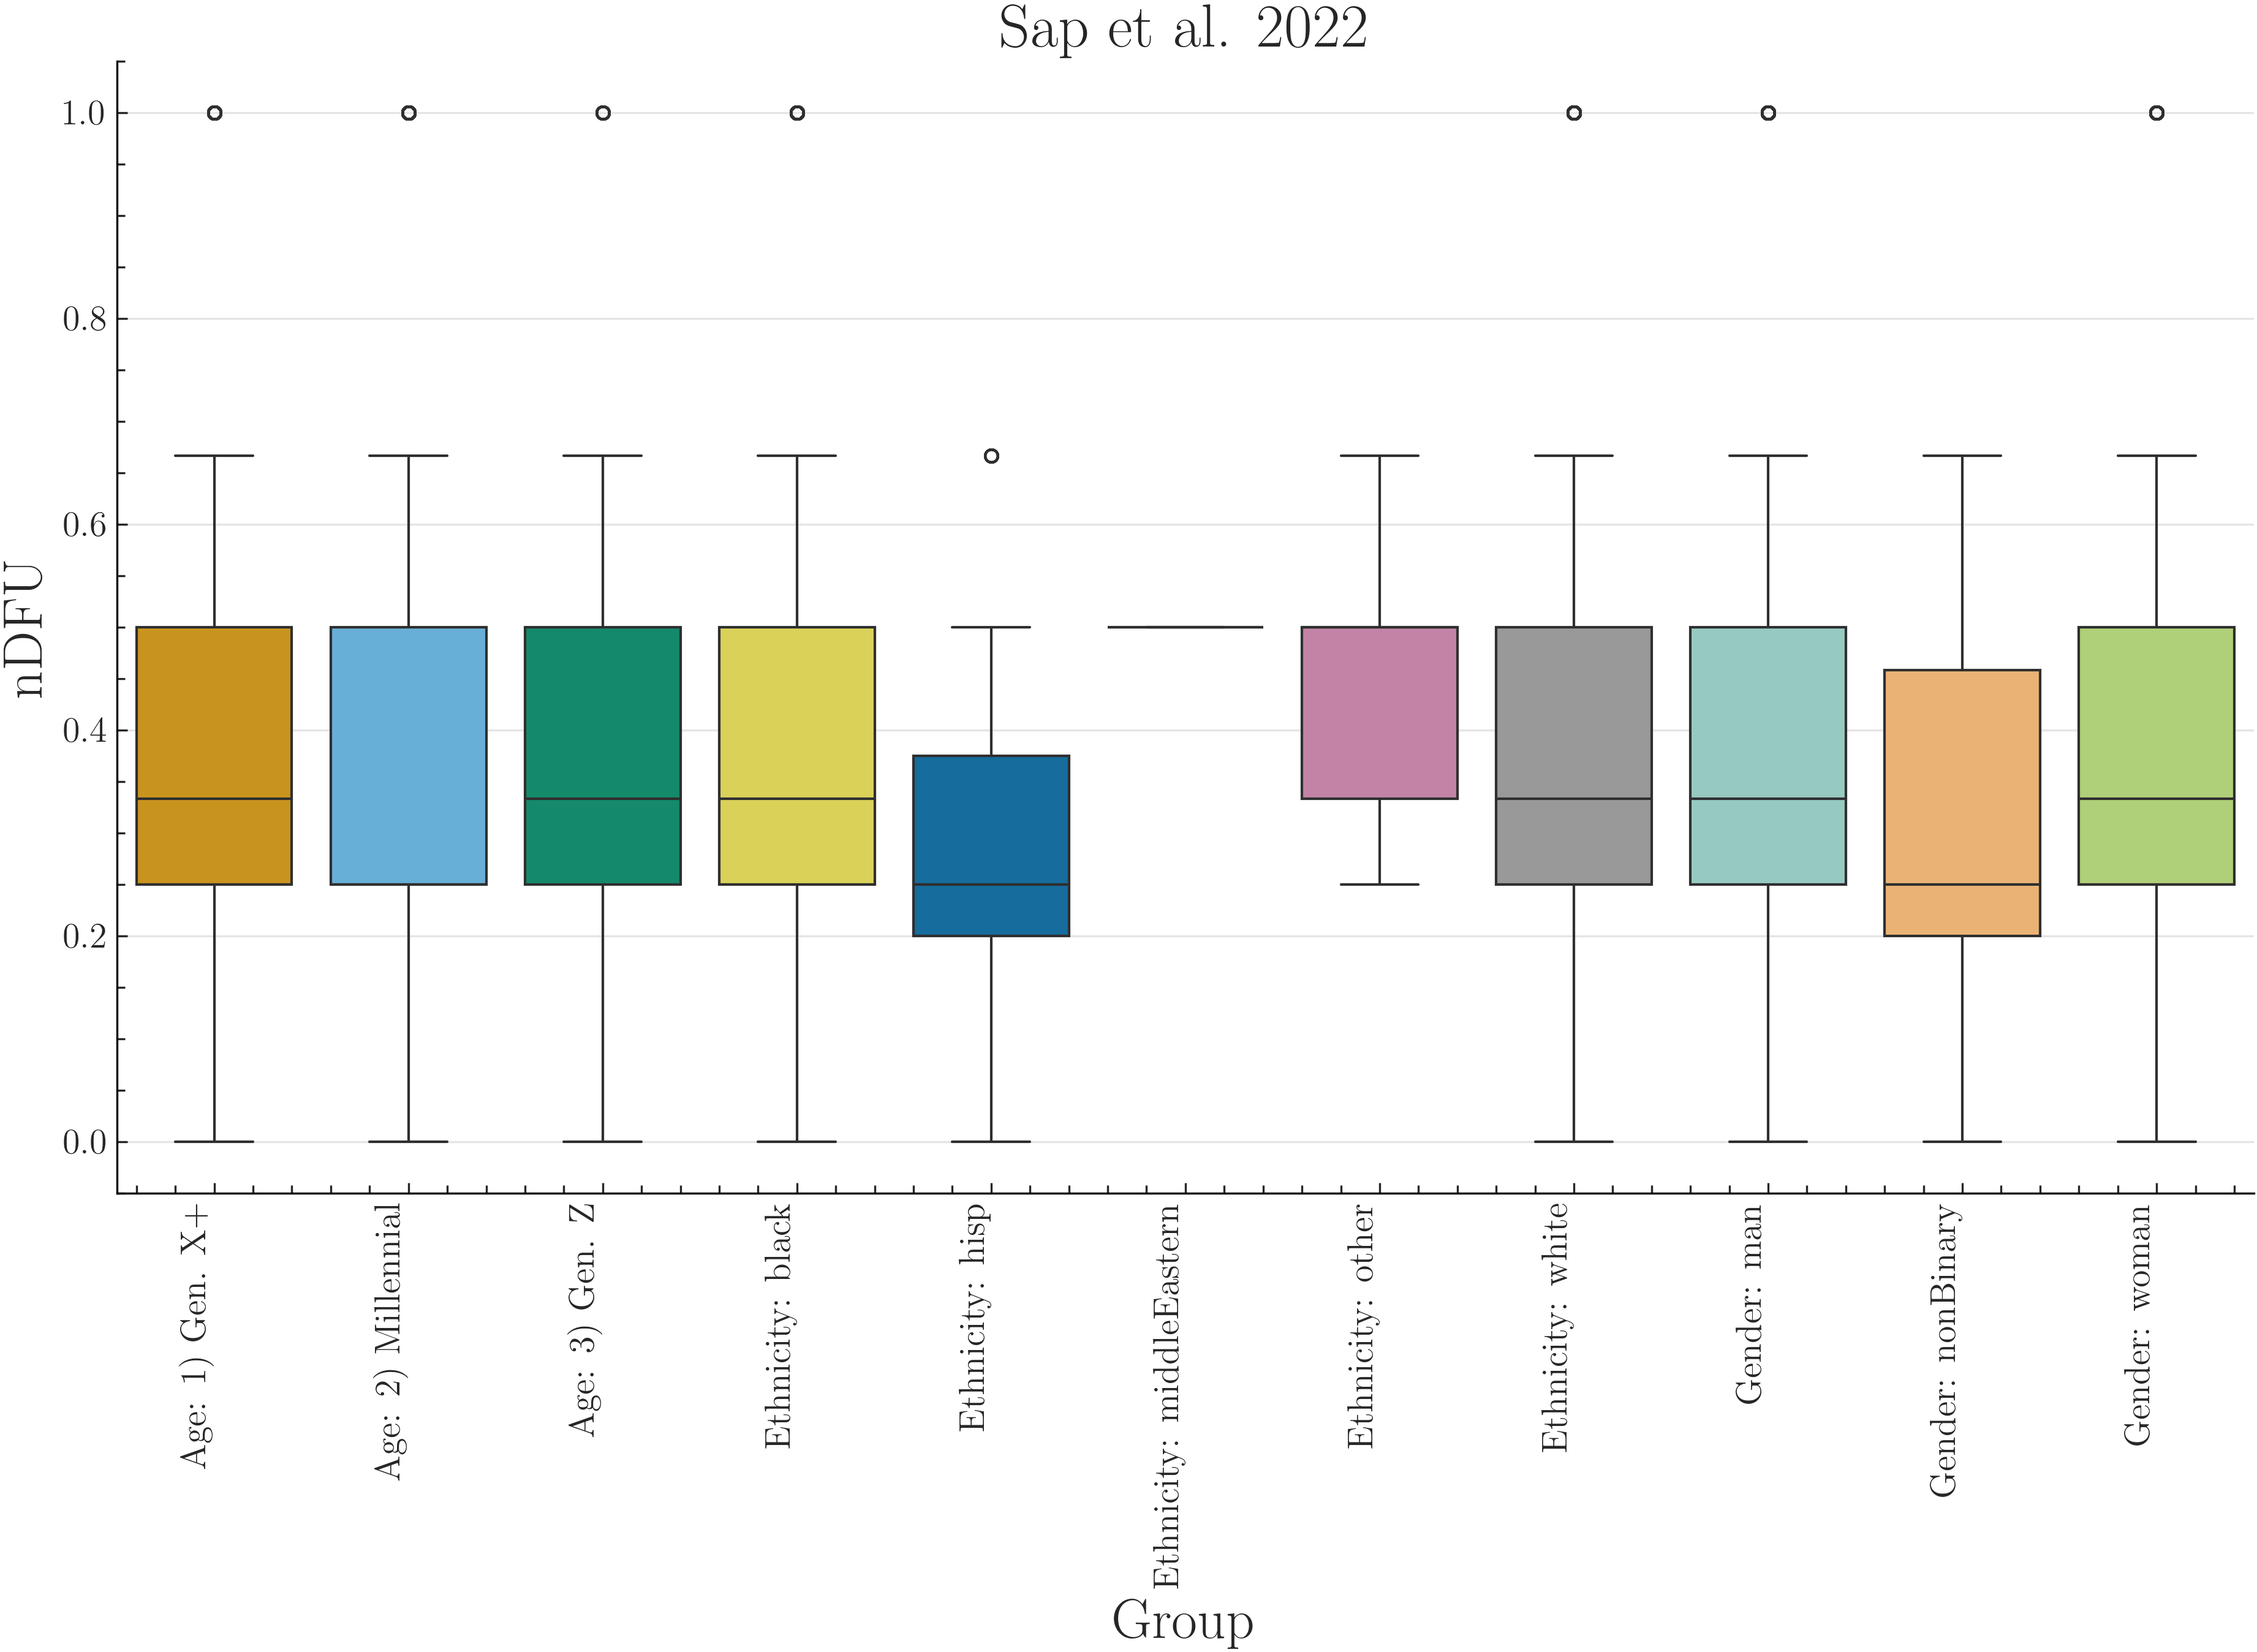
\includegraphics[width=0.48\textwidth]{sap.png}
	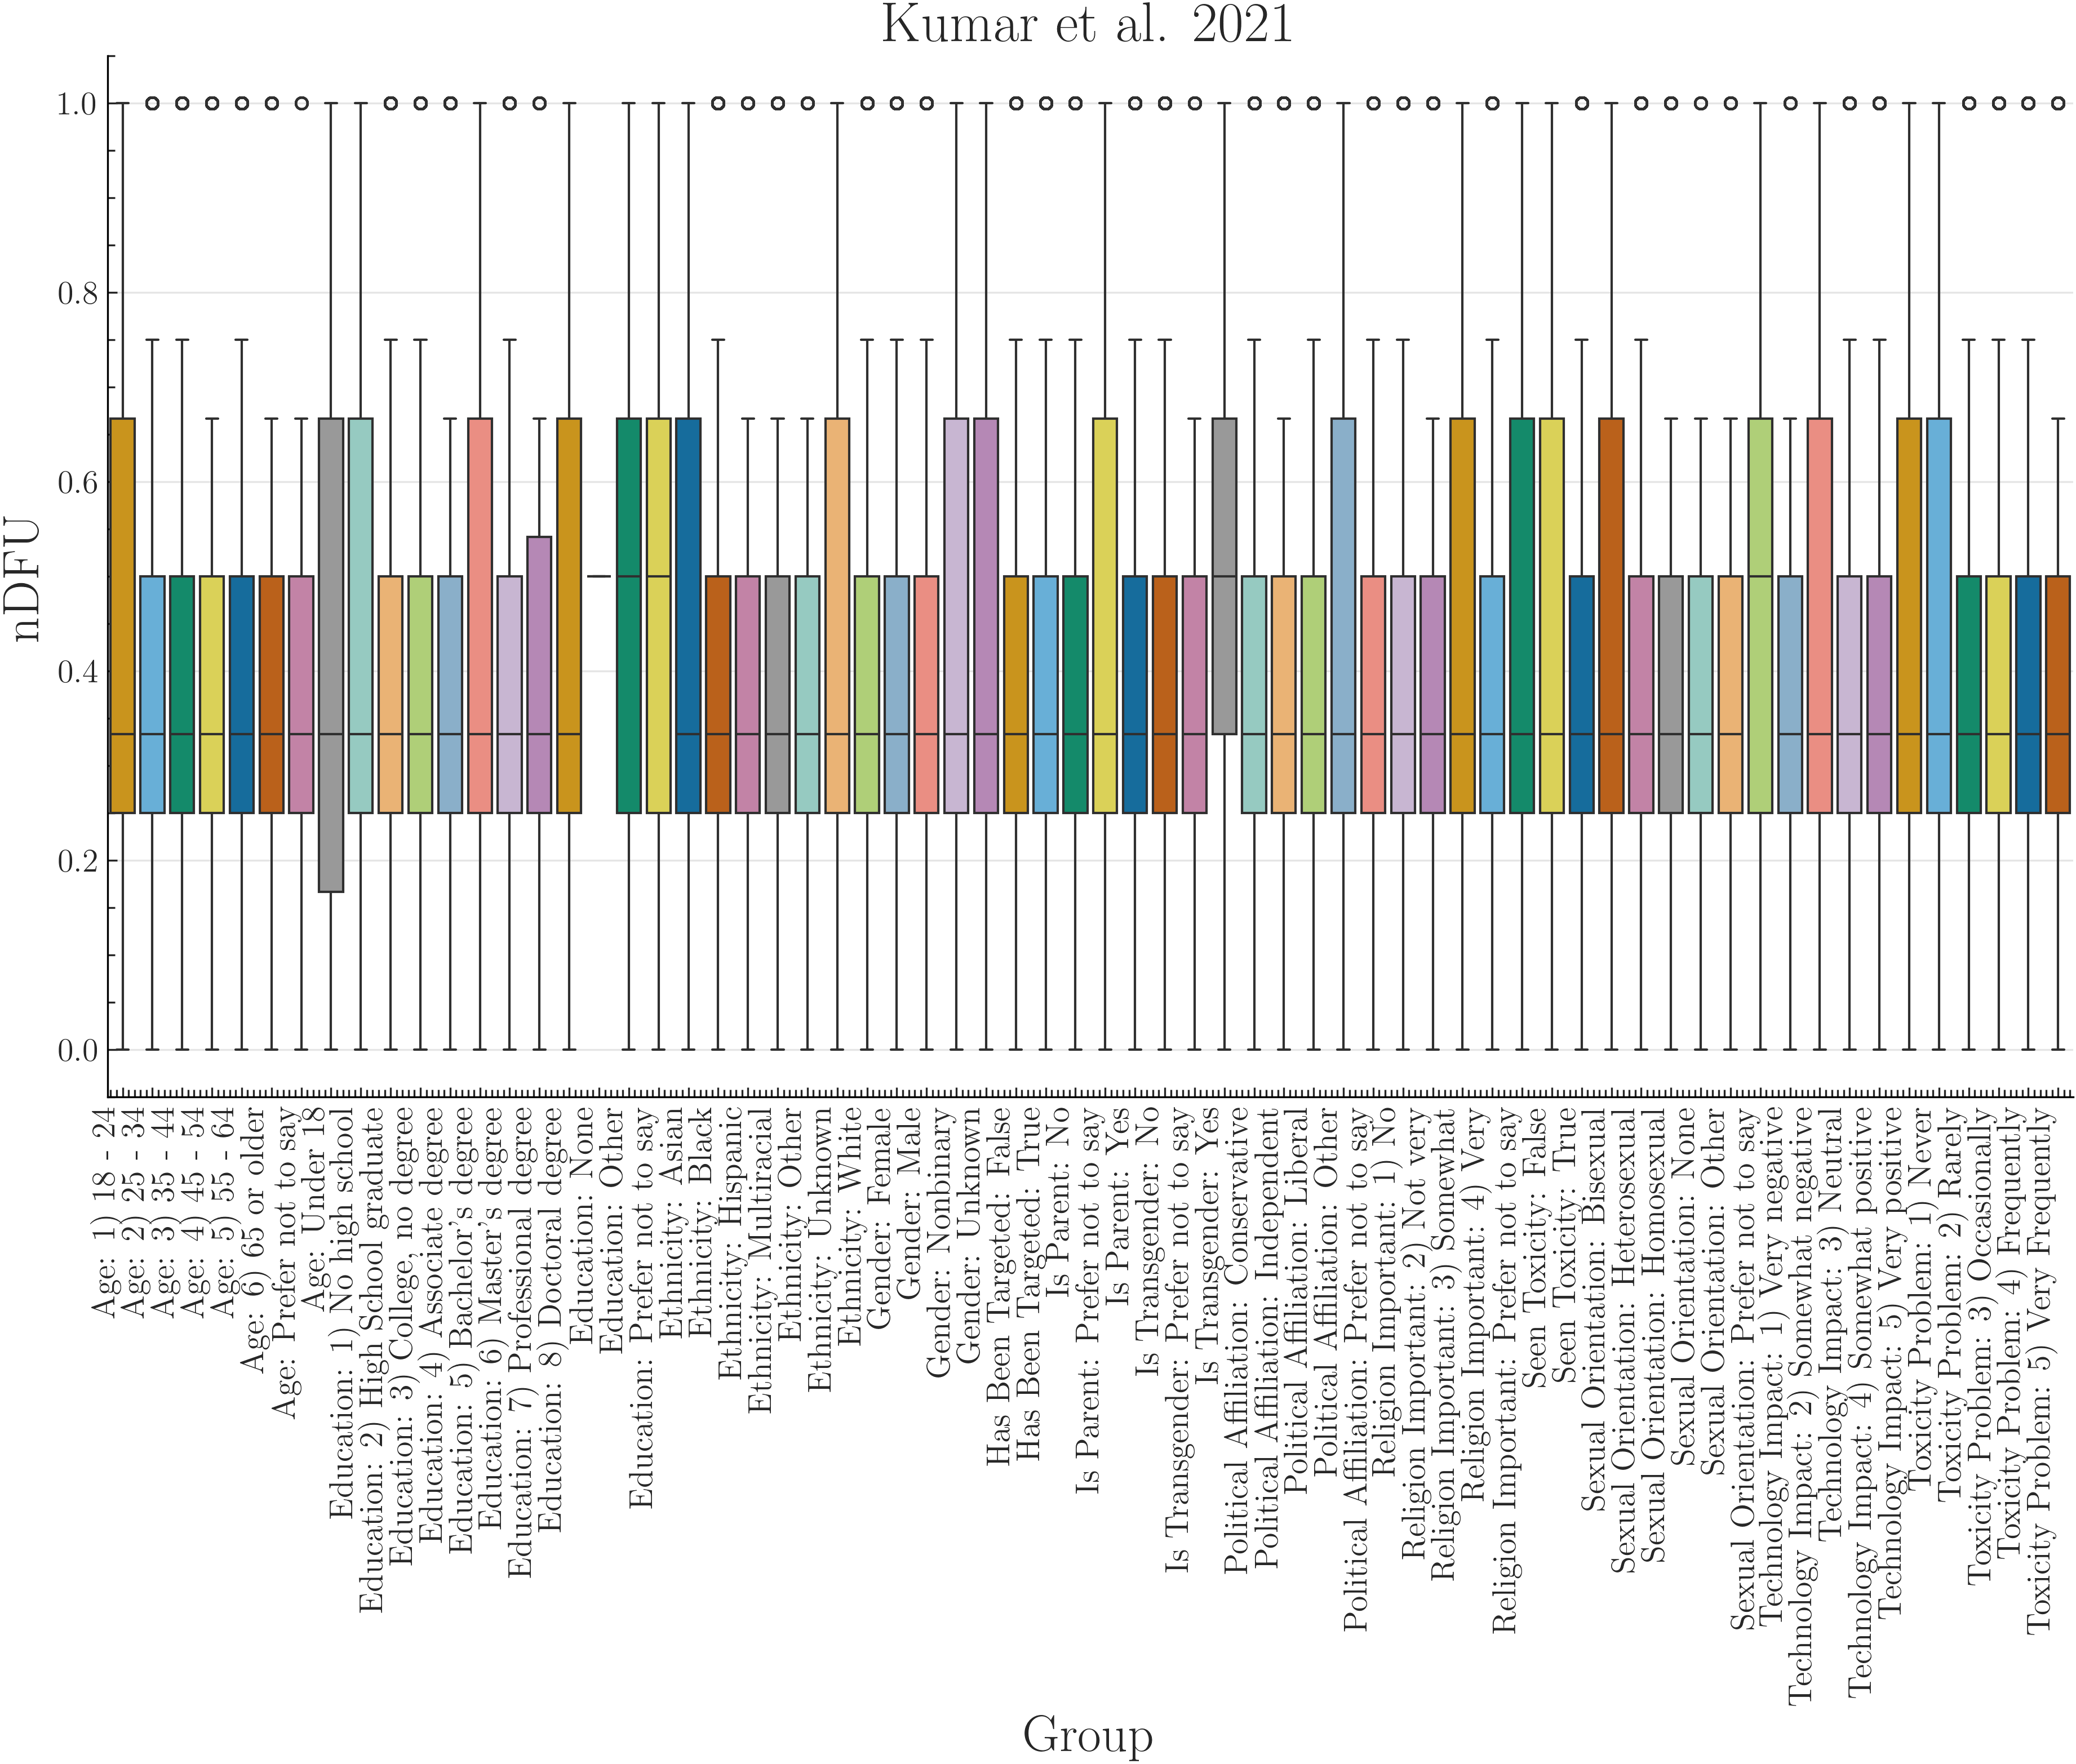
\includegraphics[width=0.48\textwidth]{kumar_sample.png}
	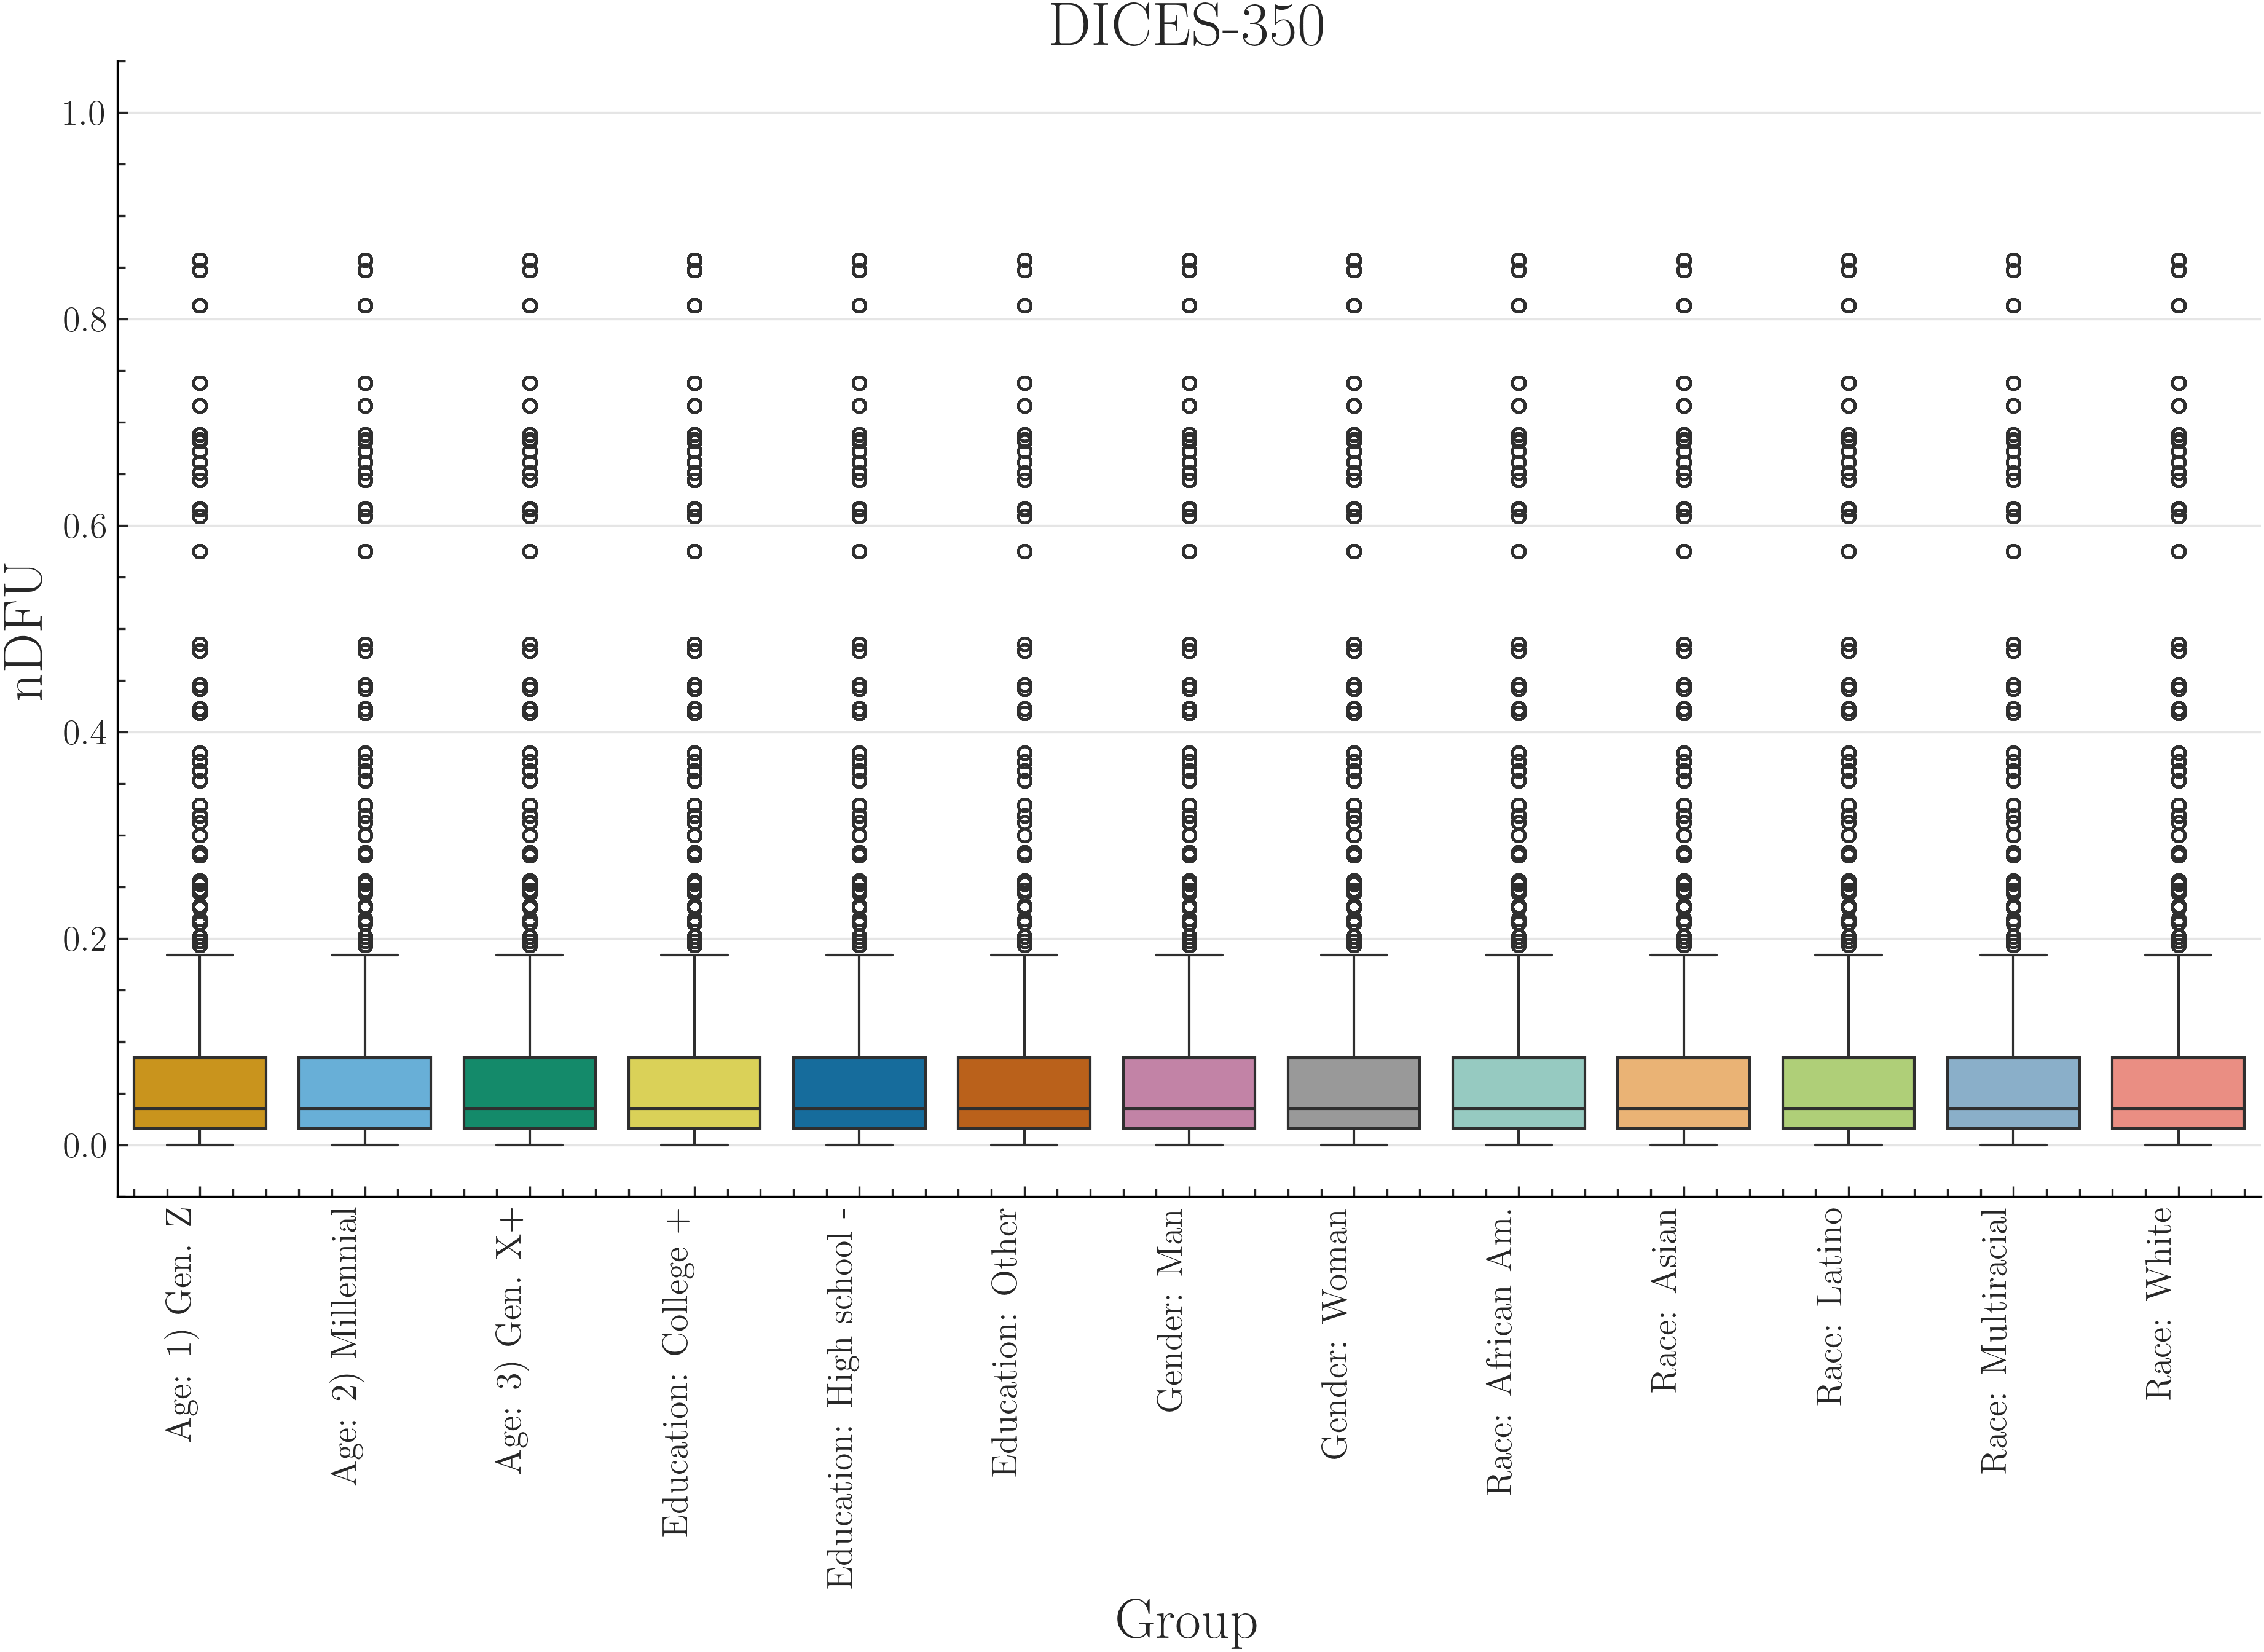
\includegraphics[width=0.48\textwidth]{dices-350.png}
	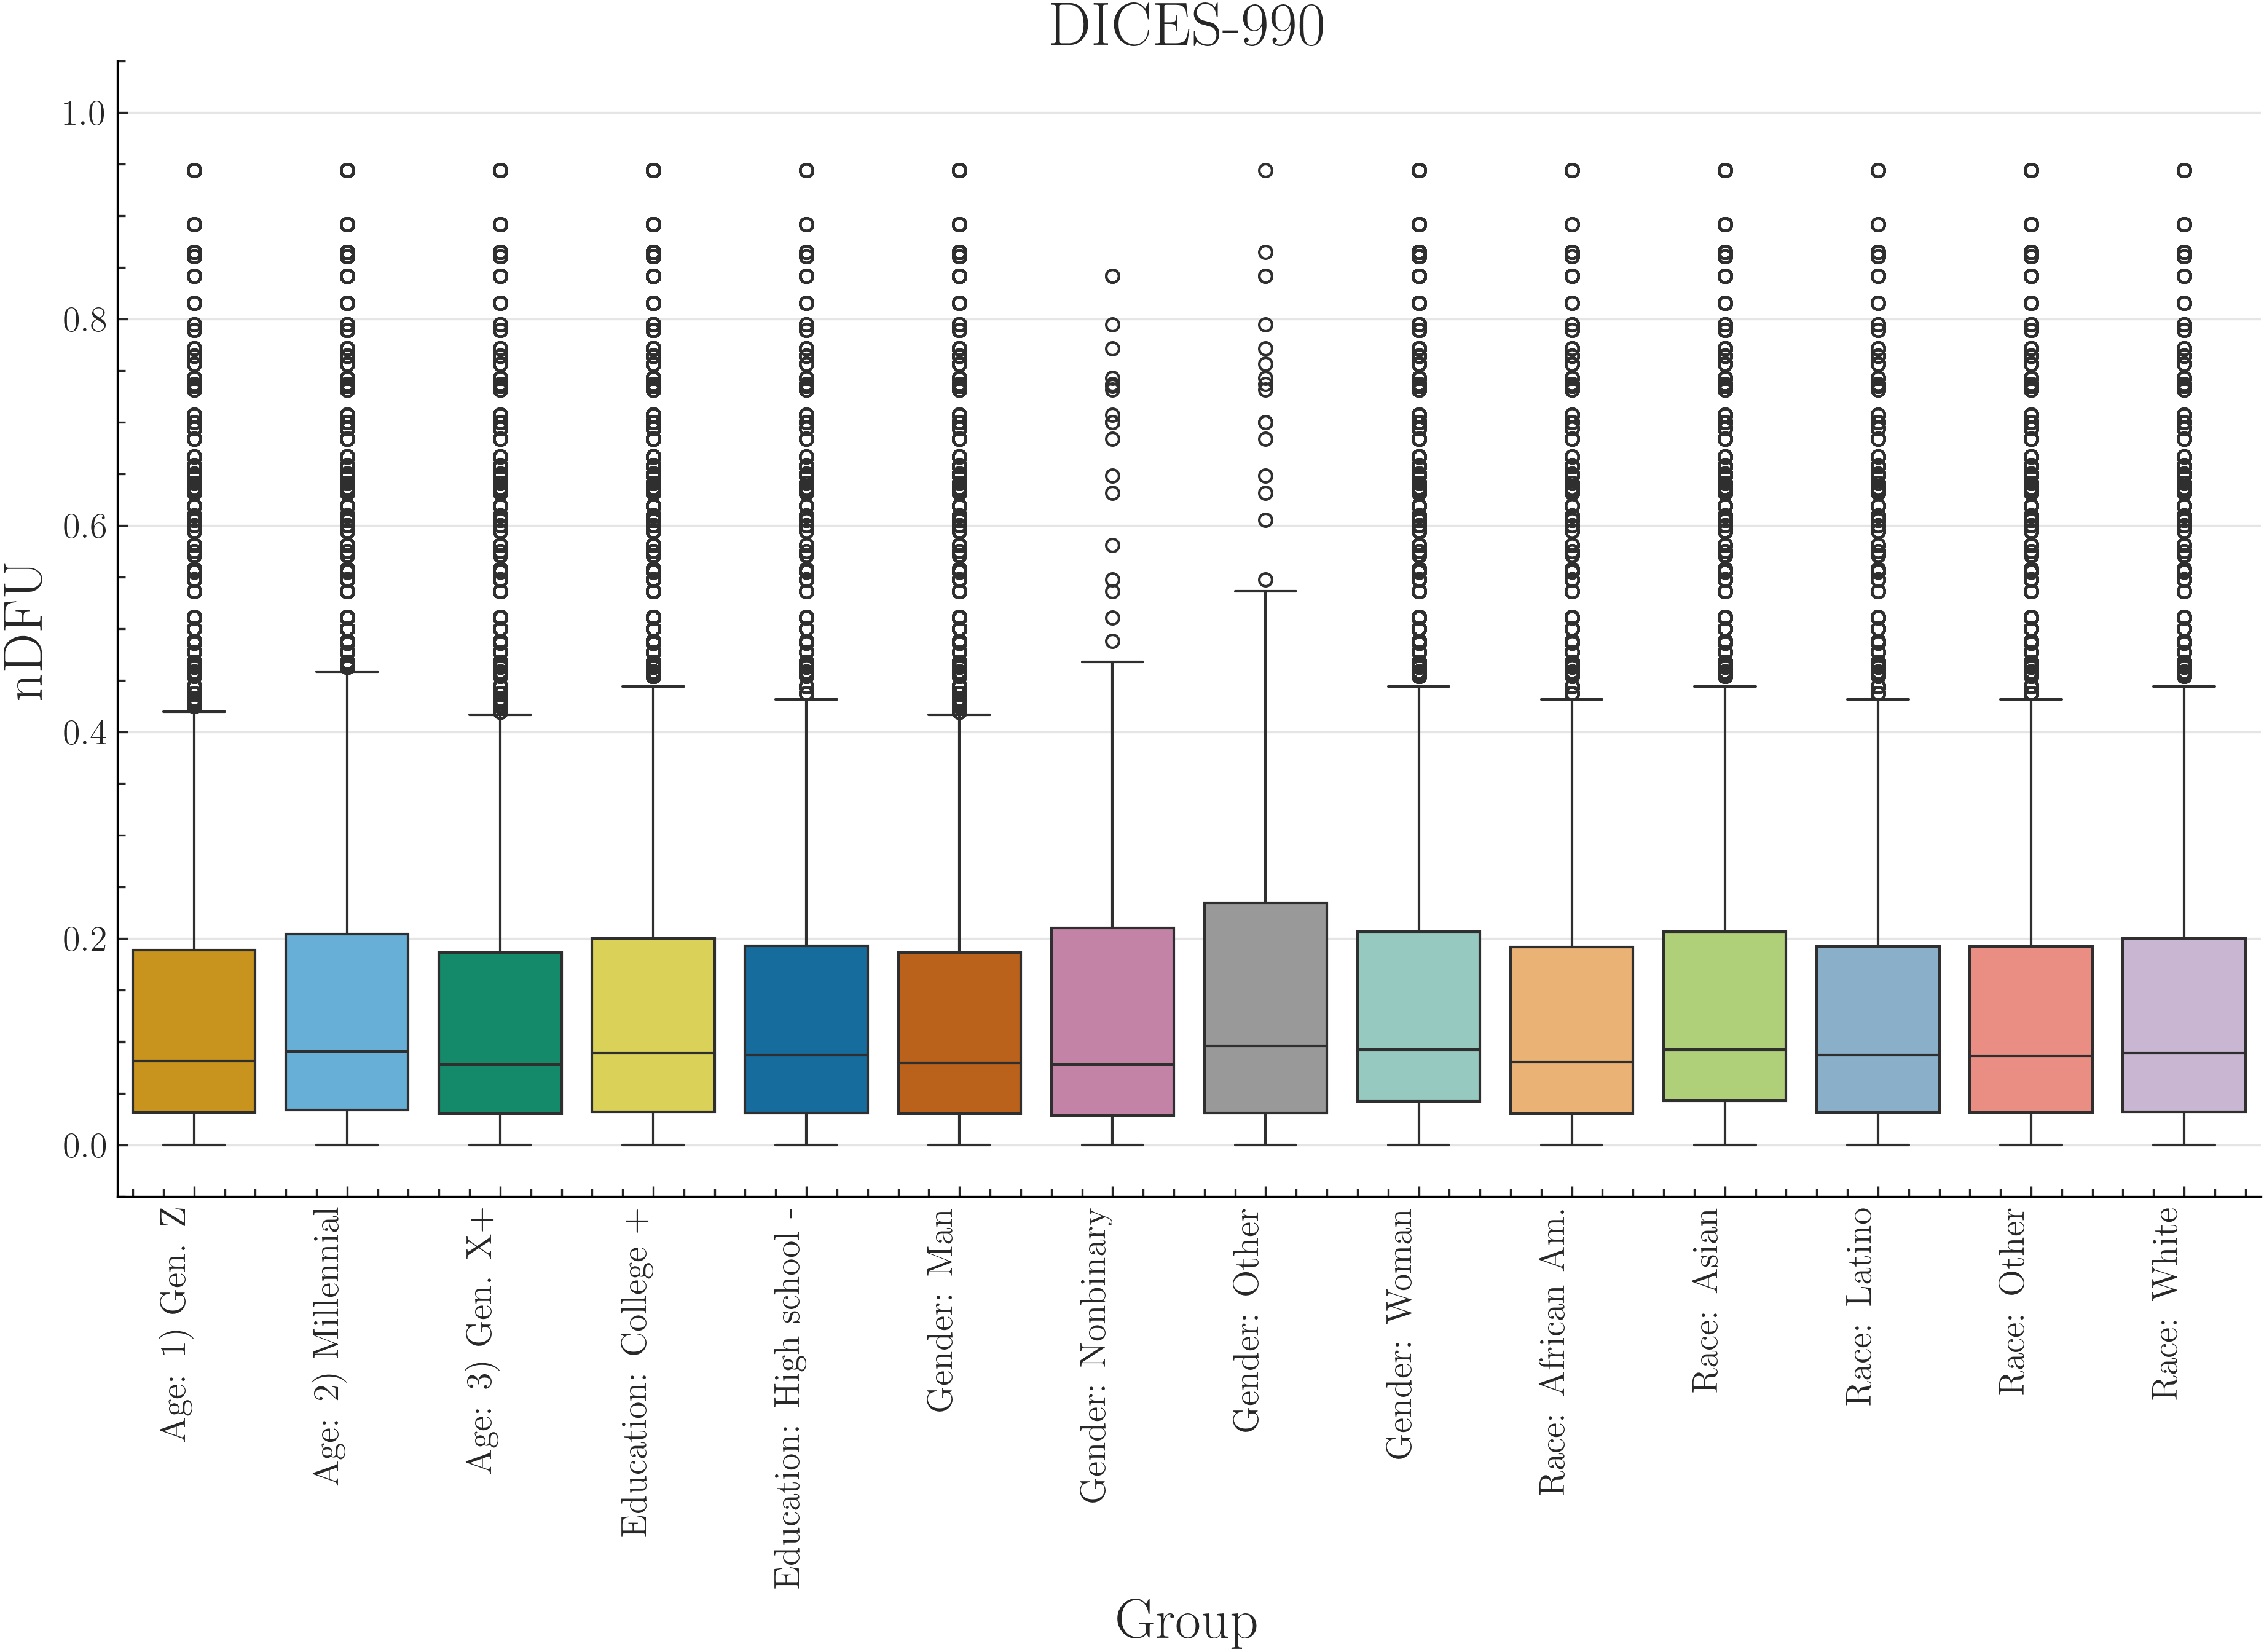
\includegraphics[width=0.48\textwidth]{dices-990.png}
	\caption{Boxplots of dataset polarization for the human datasets considered in this paper for all groups in each examined \ac{pc} dimension.}
	\label{fig:dataset-polarization}
\end{figure}


\begin{figure}[t]
	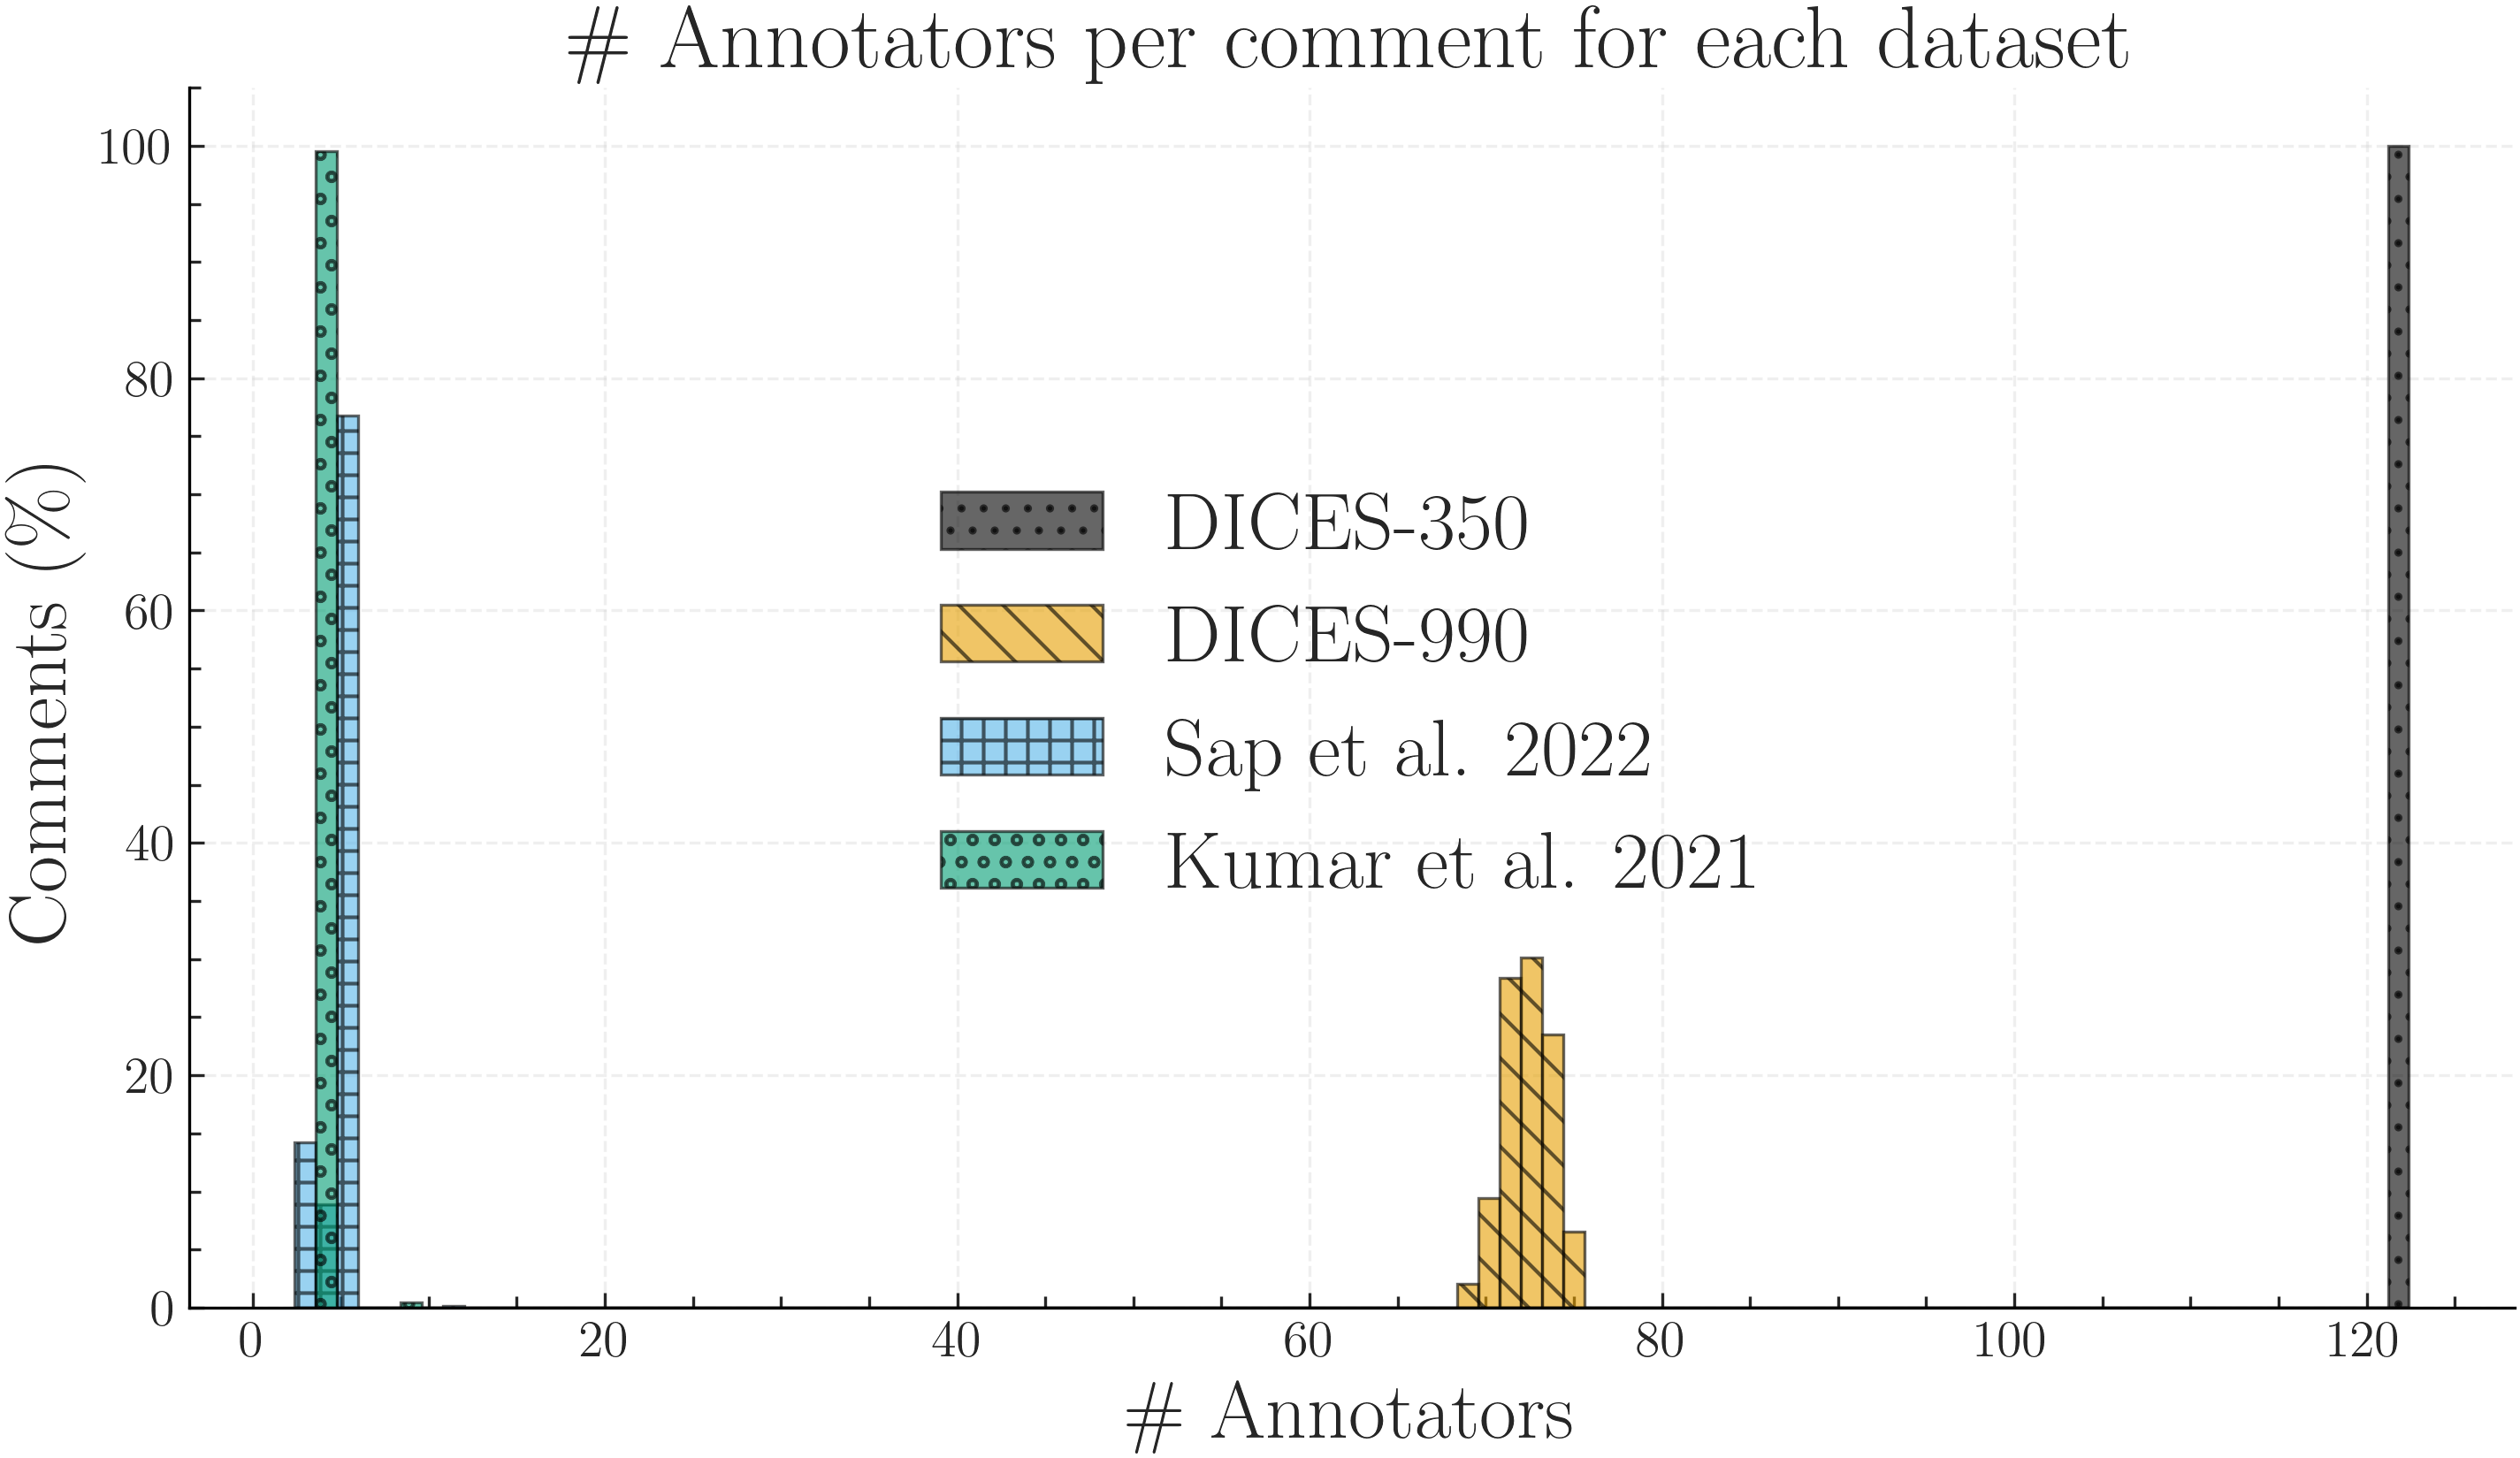
\includegraphics[width=0.55\textwidth]{annotator_count_histogram.png}
	\caption{We calculate the ratio of comments for each dataset (y-axis) that had $x$ number of annotators (x-axis). We truncate the x-axis to 130 annotators, disregarding very few comments in the Kumar dataset exceeding this threshold (see Table~\ref{tab:num-annot}), which is likely caused by a data error.}
	\label{fig:ann_counts}
\end{figure}

\begin{table}[t]
	\centering
	\begin{tabular}{lrrrrrrrr}
		\toprule
		\textbf{Dataset} & count & mean & \ac{sd} & min & 25\% & 50\% & 75\% & max \\
		\midrule
		DICES-350 & 350 & 123 & 0 & 123 & 123 & 123 & 123 & 123 \\
		DICES-990 & 990 & 72.8& 1.17 & 69 & 72 & 73 & 74 & 76 \\
		Sap & 585 & 5.6 & .78 & 3 & 6 & 6 & 6 & 12 \\
		Kumar  & 2998 & 5.02 & .34 & 5 & 5 & 5 & 5 & 10 \\
		\bottomrule
	\end{tabular}
	\caption{Number of annotations per item in each of the four datasets used in this study.}
	\label{tab:num-annot}
\end{table}

The number of annotators per comment for all datasets presented in \S\ref{sec:datasets} can be found in ~\ref{fig:ann_counts}, and descriptive statistics can be found in Table~\ref{tab:num-annot}. The DICES-990 dataset has exactly 123 annotations per comment, while the other datasets exhibit a few variations around the central mean reported in Table~\ref{tab:datasets}. Interestingly, the sample used from the Kumar dataset exhibits a few comments that vastly exceed the promised $5$ number of annotators. We do not include these comments, since they are very likely a data error. Tables~\ref{tab:dices350-stats},\ref{tab:dices990-stats},\ref{tab:sap-stats},\ref{tab:kumar-stats1},\ref{tab:kumar-stats2} show the annotation counts for each \ac{pc} group in each dataset.

\begin{table}[ht]
	\centering
	\begin{tabular}{llc}
		\toprule
		\textbf{Category} & \textbf{Subgroup}  & \textbf{Support}\\
		\midrule
		Gender & Woman & 21700 \\
		& Man & 21350 \\
		\midrule
		Race & White & 10500 \\
		& African Am. & 10150 \\
		& Asian & 9100 \\
		& Latino & 7700 \\
		& Multiracial & 5600 \\
		\midrule
		Age & 1) Gen. Z & 19600 \\
		& 2) Millennial & 12600 \\
		& 3) Gen. X+ & 10850 \\
		\midrule
		Education & College + & 26250 \\
		& High school - & 14350 \\
		& Other & 2450 \\
		\bottomrule
	\end{tabular}
	\caption{Subgroup Counts for DICES-350. ``Support'' refers to annotation count.}
	\label{tab:dices350-stats}
\end{table}

\begin{table}[ht]
	\centering
	\begin{tabular}{llc}
		\toprule
		\textbf{Category} & \textbf{Subgroup} & \textbf{Support} \\
		\midrule
		Gender & Woman & 36050 \\
		& Man & 35392 \\
		& Nonbinary & 331 \\
		& Other & 330 \\
		\midrule
		Race & Other & 26394 \\
		& Asian & 19885 \\
		& White & 12322 \\
		& Latino & 7170 \\
		& African Am. & 6332 \\
		\midrule
		Age & Gen. Z & 14899 \\
		& Millennial & 41542 \\
		& Gen. X+ & 15662 \\
		\midrule
		Education & College + & 64054 \\
		& High school - & 8049 \\
		\bottomrule
	\end{tabular}
		\caption{Subgroup Counts for DICES-990. ``Support'' refers to annotation count.}
	\label{tab:dices990-stats}
\end{table}


\begin{table}[t]
	\centering
	\begin{tabular}{llc}
		\toprule
		\textbf{Category} & \textbf{Subgroup} & \textbf{Support}\\
		\midrule
		Age& Gen. Z & 252 \\
		& Millennial & 2259 \\
		& Gen. X+ & 786 \\
		\midrule
		Ethnicity & white & 2168 \\
		& black & 1091 \\
		& hisp & 32 \\
		& other & 5 \\
		& middleEastern & 1 \\
		\midrule
		Gender & man & 1859 \\
		& woman & 1412 \\
		& nonBinary & 26 \\
		\bottomrule
	\end{tabular}
		\caption{Subgroup Counts for Sap et al. 2022. ``Support'' refers to annotation count.}
	\label{tab:sap-stats}
\end{table}

\begin{table}[t]
	\centering
	\small
	\begin{tabular}{llc}
		\toprule
		\textbf{Category} & \textbf{Subgroup} & \textbf{Support}\\
		\midrule
		\multirow{4}{*}{Gender} & Female & 8011 \\
		& Male & 6832 \\
		& Unknown & 124 \\
		& Nonbinary & 93 \\
		\midrule
		\multirow{7}{*}{Ethnicity} & White & 10699 \\
		& Black & 1940 \\
		& Asian & 862 \\
		& Multiracial & 664 \\
		& Hispanic & 418 \\
		& Other & 247 \\
		& Unknown & 230 \\
		\midrule
		\multirow{9}{*}{Age} & Under 18 & 3 \\
		& 18 - 24 & 1711 \\
		& 25 - 34 & 5969 \\
		& 35 - 44 & 3785 \\
		& 45 - 54 & 1977 \\
		& 55 - 64 & 1101 \\
		& 65 or older & 471 \\
		& N/A & 43 \\
		\midrule
		\multirow{10}{*}{Education} & No high school & 71 \\
		& High School graduate & 1353 \\
		& College, no degree & 3090 \\
		& Associate degree & 1676 \\
		& Bachelor's degree & 6071 \\
		& Master's degree & 2261 \\
		& Professional degree & 236 \\
		& Doctoral degree & 198 \\
		& N/A & 71 \\
		& Other & 32 \\
		\midrule
		\multirow{5}{*}{Sexual Orient.} & Heterosexual & 12391 \\
		& Bisexual & 1665 \\
		& Homosexual & 515 \\
		& N/A & 302 \\
		& Other & 131 \\
		\bottomrule
	\end{tabular}
	\caption{Subgroup Counts for the Kumar et al. 2021 dataset. Part 1 of 2. ``Support'' refers to annotation count.}
	\label{tab:kumar-stats1}
\end{table}


\begin{table}[t]
	\centering
	\small
	\begin{tabular}{llc}
		\toprule
		\textbf{Category} & \textbf{Subgroup} & \textbf{Support}\\
		\midrule
		\multirow{3}{*}{Is Transgender} & No & 14549 \\
		& Yes & 363 \\
		& N/A & 148 \\
		\midrule
		\multirow{5}{*}{Politics} & Liberal & 5997 \\
		& Independent & 4143 \\
		& Conservative & 3981 \\
		& N/A & 609 \\
		& Other & 330 \\
		\midrule
		\multirow{3}{*}{Is Parent} & Yes & 7889 \\
		& No & 7015 \\
		& N/A & 156 \\
		\midrule
		\multirow{5}{*}{Tech Impact} & Very negative & 149 \\
		& Somewhat negative & 1411 \\
		& Neutral & 1905 \\
		& Somewhat positive & 7690 \\
		& Very positive & 3905 \\
		\midrule
		\multirow{5}{*}{Tox Problem} & Never & 869 \\
		& Rarely & 2485 \\
		& Occasionally & 5307 \\
		& Frequently & 4441 \\
		& Very Frequently & 1958 \\
		\midrule
		\multirow{5}{*}{Rel Important} & No & 4735 \\
		& Not very & 1808 \\
		& Somewhat & 3548 \\
		& Very & 4741 \\
		& N/A & 228 \\
		\midrule
		\multirow{2}{*}{Seen Toxicity} & True & 11505 \\
		& False & 3555 \\
		\midrule
		\multirow{2}{*}{Has Been Target} & False & 10741 \\
		& True & 4319 \\
		\bottomrule
	\end{tabular}
	\caption{Subgroup Counts for Kumar et al. 2021 dataset. Part 2 of 2. ``Support'' refers to annotation count.}
	\label{tab:kumar-stats2}
\end{table}


\section{Statistical considerations}
\label{app:stats}

\subsection{Defining apriori polarization}
\label{app:stats:comparison}

In \S\ref{sec:inherent:formulation}, we explained how our methodology needs to compare the polarization of $A(c)$ and $A(c \given g)$. Direct comparisons are not advisable, since we would be comparing statistics between a set and its subset---in this case, standard practice dictates comparing the subset with its complement; i.e., the in-group vs. the out-group instead of the in-group vs. all the annotations. However, this also would not work; if we apply the subset-vs-complement method in the example of Fig.~\ref{fig:ndfu_combined}, we would end up subtracting the \acp{ndfu} of men and women, which are similar as they are both unimodal distributions, falsely concluding that there is no polarization present.


\subsection{Filtering ineligible comments}
\label{app:stats:filtering}

Because \textit{apunim} is fundamentally designed to quantify polarization, we exclude comments that exhibit no measurable polarization ($nDFU(c)=0$). Furthermore, we also exclude comments annotated exclusively by a single group (i.e., comments where there are no two groups with at least three annotators each), since we require valid histograms for the non-parametric estimation of \ac{ndfu} (see Eq.~\ref{eq:ndfu}). This is an unfortunately common scenario, since many \ac{nlp} datasets feature only $5-6$ annotations per comment. In a best-case scenario of 5 annotators split evenly between two groups, we would get a 3-2 split.


\subsection{P-value estimation}
\label{app:stats:pvalue}

Since our test is parametric (\S\ref{sec:apunim:statistical}), it assumes that there exist (1) enough data-points to reliably run the means-test, (2) enough annotations per \ac{pc} group to estimate \acp{ndfu} in Equations~\ref{eq:apriori}-\ref{eq:observed}, (3) the apunims of the random partitions are independent and identically distributed. Condition (1) can be safely assumed for most datasets, because they feature enough items to reliably assume normal residuals (see \S\ref{sec:datasets}). We discuss condition (2) in App.~\ref{sec:ideal-dataset}. Condition (3) is partly fulfilled; the partitions are identically distributed, but may be dependent on the sample distribution. 

Replacing the parametric means test with a non-parametric alternative would relax assumptions about the underlying distribution but would not resolve the potential dependence between the random apunims. We initially attempted to implement a permutation test on the empirical (random apunim) distribution, but this resulted in excessive computational costs.

While the test operates on a single group in principle, in practice we often want to test polarization for all subgroups of a specific dimension. Since we are simultaneously considering multiple hypotheses, we apply a multiple comparison correction to the resulting p-values---specifically the Holms method~\cite{holms}. The test is parameterized by the confidence level of our test, which is used to tune the strength of the correction; we can increase this value to make our test more conservative towards multiple hypotheses~\cite{ChenFengYi2017}).


\section{Software}
\label{app:software}

\subsection{Installation and usage}
We release the \texttt{apunim} package, which is a Python library that implements both the \ac{ndfu} and apunim calculations, as well as its statistical test. The software is available on PyPi We also provide high-level documentation in HTML format that includes an introduction, guide, and full low-level documentation for each of the two provided functions (\doclink).

The code is open-source, licensed under the \ac{gpl} and can be found on the project's repository (\explink). The library is cross-platform, works for any Python 3 version, and requires very few dependencies (namely \texttt{numpy, scipy, statsmodels}).

\subsection{Implementation details}
By default, the computation of the apunim values happens on a single thread. In cases of serious computational cost, we recommend running the apunim calculation on multiple concurrent processes, since all operations are CPU-bound and thread-safe. This may be useful in cases where there are multiple \ac{pc} dimensions, each of which is computationally expensive. 

In order to lower the computational cost required, we re-use the random partitions $\tilde{r}_i$, which are originally calculated to obtain the apriori polarization values (see Eq.~\ref{eq:apriori}), for the p-value calculations (\S\ref{sec:apunim:statistical}). This means that in our current implementation, the number of groups for estimating apriori polarization ($\tilde{r}_i$ in Eq.~\ref{eq:apriori}), and the number of apunim values used in the p-value calculation have to be the same.


\section{Replication details}
\label{app:replication}

We use version \texttt{1.0.5} of the \texttt{apunim} library for our experiments. We use 100 random iterations for the apriori value calculation (Eq.~\ref{eq:apriori}) and the p-value estimation (\S\ref{sec:apunim:statistical}), and set a confidence level of $\alpha=0.05$.

While the library efficiently handles large numbers of annotators through vectorized operations, performance degrades significantly when processing a high volume of comments, particularly when annotators belong to multiple distinct groups. For instance, while experiments across all datasets in \S\ref{sec:datasets} complete within a minute, the Kumar dataset necessitates approximately one hour of computation using commercial hardware. Furthermore, the annotator variance analysis detailed in App.~\ref{sec:ideal-dataset} required over ten hours. While this latter time requirement is anticipated due to the inherently demanding nature and non-standard application of our library, it demonstrates the existence of a potential scaling bottleneck. The same applies to a lesser extent for the subsampling experiments on the DICES datasets, taking collectively three hours of computation.

We hypothesize that this bottleneck is likely caused by repeated creation of numpy arrays, resulting in repeated memory allocations for each subgroup, in each comment, for each \ac{pc} dimension. We plan on profiling and addressing it in the next releases of our software. Until then, we suggest either using multiprocessing for each \ac{pc} subgroup, or running the different experiments in parallel (indeed, we use the \texttt{gnu-parallel} package~\cite{tange_2025_16944306} for our own experiments). We also note that the Kumar dataset also requires substantial RAM resources, estimated around 42--46GB of dedicated RAM should the whole dataset be considered.

Finally, we note that in Fig.~\ref{fig:std_error}, we removed values where there was a lack of items annotated by the specified number of annotators (e.g., only 7\% of comments in DICES-990 were annotated by more than 73 annotators---see App.~\ref{app:ann_details}).


\section{Synthetic experiments}
\label{app:experiments}

This appendix details the synthetic experiments used to illustrate the functionality and behavior of \ac{ndfu}. In all simulations, the bin size is set to $N_{bins}=10$.

\paragraph{Disagreement vs. polarization}
To explore the relationship between annotation polarization and disagreement in Fig.~\ref{fig:disagreement-vs-polarization}, we constructed a $2 \times 2$ matrix of synthetic datasets, each drawing from a pool of $N_{annotators}=100$. Polarization is simulated by defining a minority group, which constitutes $20\%$ of the total annotators ($\text{n\_special}=20$). These minority annotators are assigned a targeted mean shift ($\text{mean\_shift}=1$) from the base distribution. The base variance for these distributions is set at $\text{variance}=0.3$. Different types of distributions (unimodal, bimodal, multimodal, uniform) are achieved by controlling the $\text{base\_means}$ and applying variance multipliers (e.g., $\text{variance} \times 3$ for multimodal).

\paragraph{Single-comment polarization}
We simulate the distribution of toxicity annotations in Fig.~\ref{fig:ndfu_combined} across two demographic groups (Men and Women). The distribution of Men's scores is modeled using a truncated normal distribution with $\text{loc}=2$ and $\text{scale}=1.3$, while Women's scores are modeled with $\text{loc}=8$ and $\text{scale}=1.3$. The combined dataset, representing all annotations, is used to demonstrate the impact of population weighting on the overall nDFU score. The sample size for each group in this visualization is $N_{annotators}=50$.

\paragraph{Discussion-level polarization}
We examine nDFU scores for three specific textual examples presented in Fig.~\ref{fig:ndfu_discussion}. For the individual comments, $N_{annotators}=200$ for each group. In the first case (misogynist comment), Men's scores are modeled with $\text{loc}=6$, while Women's scores are modeled with $\text{loc}=2$. In the second case (misandrist comment), the roles are reversed. The third visualization combines distributions for men and women derived from the respective single-comment distributions.


\section{How does InPol look like?}
\label{app:inherent}

\begin{table}[ht]
	\begin{tabularx}{\textwidth}{X c}
		\toprule
		\textbf{Comment}  & \ac{ip} \\
		\midrule
		The minks mentioned in the headline are indeed "rising" from where they were based, but that is due to them being buried in shallow mass graves (Africa) and filling with gas that causes them to rise out.  Rest assured, they're still very much dead, thankfully!. & 1 \\
		There should be such thing as a bitch resistance for us women  & 1\\
		There's a big difference between being a bitch and being a woman & 1 \\
		i just watched a video of @joisnotonfire being an annoying hoe on skype i'm laughing & 1 \\
		niggas love to commit crime & 1 \\
		\midrule
		I swear to God above I love ya and when ya be with this brotha, I swear I love you my bro as long as you not a nigga & 0.5 \\
		I will become a cold ass bitch because of my treatment & 0.5\\
		I would happily lay out a nigga & 0.5\\
		Shoot yourself in the head you hypersensitive fuckin bitch.  & 0.5 \\
		not all women are bitches, but all bitches are women & 0.5 \\
		\midrule
		`` you ugly bitch!!!"- that seems to be my real name these days'' & 0 \\
		``I am happy to report that drowning does kill this demonic entity. Oh holy are the waters of Chernarus!"" Omg, DED ;)''& 0\\
		``Let them praise the name of the LORD: for his name alone is excellent; his glory is above the earth and heaven."" ~Psalms 148:13 \#Bible''& 0\\
		someone plz get this nigger some help. He's playing up like mad & 0\\
		stop talking you fucking nigger ! & 0 \\
		\bottomrule
	\end{tabularx}
	\caption{Sample of comments from the Sap dataset and their \ac{ip}. Note that unambiguously toxic comments can be assigned with zero \ac{ip}, while more nuanced cases tend to have higher values.}
	\label{tab:inherent-examples}
\end{table}

Table~\ref{tab:inherent-examples} shows a random sample of comments taken from the Sap dataset and their respective \ac{ip} values (\S\ref{sec:inherent:inherent}). Note that explicitly toxic or racist comments tend to have \ac{ip} values of zero, alongside clearly unproblematic comments. Inversely, more ambiguous and less comprehensible comments tend to have larger \ac{ip} values. This pattern may suggest that \ac{ip} may be tied to the overall ambiguity of the statements, especially in cases where comments may either be interpreted as very toxic, or non-toxic, which agrees with the overall goal of \ac{ndfu} (\S\ref{sec:related:polarization}).
We include the \ac{ip} values for each individual comment for all four datasets in the supplementary material.


\section{Ablation experiments}
\label{app:ablation}

\subsection{Can DICES be used for InPol?}
\label{app:ablation:dices}

In order to investigate whether the numerous annotators per comments can explain the lack of \ac{ip} in the DICES datasets (\S\ref{sec:inherent:why}) we gradually subsample the annotators for each comment randomly with replacement, starting from five annotators per comment, and scaling up to the full complement of annotators in the dataset with a step of two. For each such step, we choose ten annotator samples and compute the maximum \ac{ip} across all runs. Even with annotator counts similar to the Kumar and DICES datasets, \ac{ip} remains zero, suggesting that the absence of \ac{ip} can not be attributed to annotator number alone---rather, it is plausibly a pattern attributable to the DICES datasets themselves. 


\subsection{How does dataset size influence apunim?}
\label{app:ablation:sample-size}

\begin{table}[t]
	\scriptsize
	\centering
	\begin{tabular}{l c c c}
		\toprule
		\textbf{\ac{pc}} & \textbf{1000} & \textbf{10000} & \textbf{30000} \\
		\midrule
		% --- Age Features ---
		\multicolumn{4}{l}{\textbf{Age}} \\
		\midrule
		8 - 24 & -.002 & -.037 & -.016 \\
		25 - 34 & .045 & 0 & 0 \\
		35 - 44 & -.043 & -.001 & -.001 \\
		45 - 54 & .001 & .013 & .003 \\
		55 - 64 & .002 & -.057 & .001 \\
		65 or older & -.007 & N/A & .948 \\
		\midrule
		
		% --- Education Features ---
		\multicolumn{4}{l}{\textbf{Education}} \\
		\midrule
		High School graduate & -.023 & -.005 & .014 \\
		\textbf{College, no degree} & -.045 & .010 & .006 \\
		Associate degree & .001 & .005 & .009 \\
		Bachelor's degree & .029 & -.001 & -.000 \\
		Master's degree & .024 & .004 & -.000 \\
		\midrule
		
		% --- Ethnicity Features ---
		\multicolumn{4}{l}{\textbf{Ethnicity}} \\
		\midrule
		Asian & -.012 & .011 & .007 \\
		Black & .036 & -.004 & -.012 \\
		Hispanic & .004 & 0 & -.099 \\
		Multiracial & .008 & 0 & 0 \\
		Other & -.008 & N/A & -.306 \\
		\textbf{White} & -.023 & 0 & 0 \\
		\midrule
		
		% --- Gender Features ---
		\multicolumn{4}{l}{\textbf{Gender}} \\
		\midrule
		Female & -.006 & .002 & .001 \\
		Male & .040 & -.002 & -.001 \\
		\midrule
		
		% --- Has Been Targeted Features ---
		\multicolumn{4}{l}{\textbf{Has Been Targeted}} \\
		\midrule
		\textbf{False} & -.059 & 0 & 0 \\
		True & .017 & -.003 & -.002 \\
		\midrule
		
		% --- Is Parent Features ---
		\multicolumn{4}{l}{\textbf{Is Parent}} \\
		\midrule
		\textbf{No} & -.084 & .001 & .001 \\
		N/A & .004 & 1.000 & 0 \\
		\textbf{Yes} & .071 & 0 & 0 \\
		\midrule
		
		% --- Is Transgender Features ---
		\multicolumn{4}{l}{\textbf{Is Transgender}} \\
		\midrule
		\textbf{No} & -.102 & 0 & 0 \\
		\midrule
		
		% --- Political Affiliation Features ---
		\multicolumn{4}{l}{\textbf{Political Affiliation}} \\
		\midrule
		Conservative & .056 & -.003 & -.002 \\
		Independent & -.003 & .001 & .002 \\
		Liberal & -.026 & .001 & .001 \\
		Other & -.003 & 0 & 0 \\
		\midrule
		
		% --- Religion Important Features ---
		\multicolumn{4}{l}{\textbf{Religion Important}} \\
		\midrule
		\textbf{No} & -.071 & .002 & .001 \\
		Not very & -.013 & .010 & .006 \\
		Somewhat & .022 & .003 & -.002 \\
		\textbf{Very} & .043 & -.003 & -.002 \\
		\midrule
		
		% --- Seen Toxicity Features ---
		\multicolumn{4}{l}{\textbf{Seen Toxicity}} \\
		\midrule
		\textbf{False} & .025 & -.001 & -.001 \\
		\textbf{True} & -.082 & .001 & 0 \\
		\midrule
		
		% --- Sexual Orientation Features ---
		\multicolumn{4}{l}{\textbf{Sexual Orientation}} \\
		\midrule
		Bisexual & -.003 & -.040 & -.013 \\
		\textbf{Heterosexual} & -.067 & 0 & 0 \\
		Homosexual & -.012 & 0 & .053 \\
		\midrule
		
		% --- Technology Impact Features ---
		\multicolumn{4}{l}{\textbf{Technology Impact}} \\
		\midrule
		Somewhat negative & -.008 & 0 & .003 \\
		Neutral & .017 & -.014 & 0 \\
		Somewhat positive & -.053 & 0 & .001 \\
		Very positive & .027 & -.004 & -.003 \\
		\midrule
		
		% --- Toxicity Problem Features ---
		\multicolumn{4}{l}{\textbf{Toxicity Problem}} \\
		\midrule
		Never & -.008 & -.037 & -.081 \\
		Rarely & .004 & .003 & -.001 \\
		Occasionally & -.012 & -.003 & -.001 \\
		Frequently & -.032 & -.001 & 0 \\
		Very Frequently & -.017 & .030 & .015 \\
		\bottomrule
	\end{tabular}
	\caption{Comparison of apunim values across different sample sizes (1k, 10k, 30k) for the Kumar dataset. Bold rows show statistically significant results in the 3k sample used in the main text.}
	\label{tab:num-comments-apunim}
\end{table}

\begin{figure}[t]
	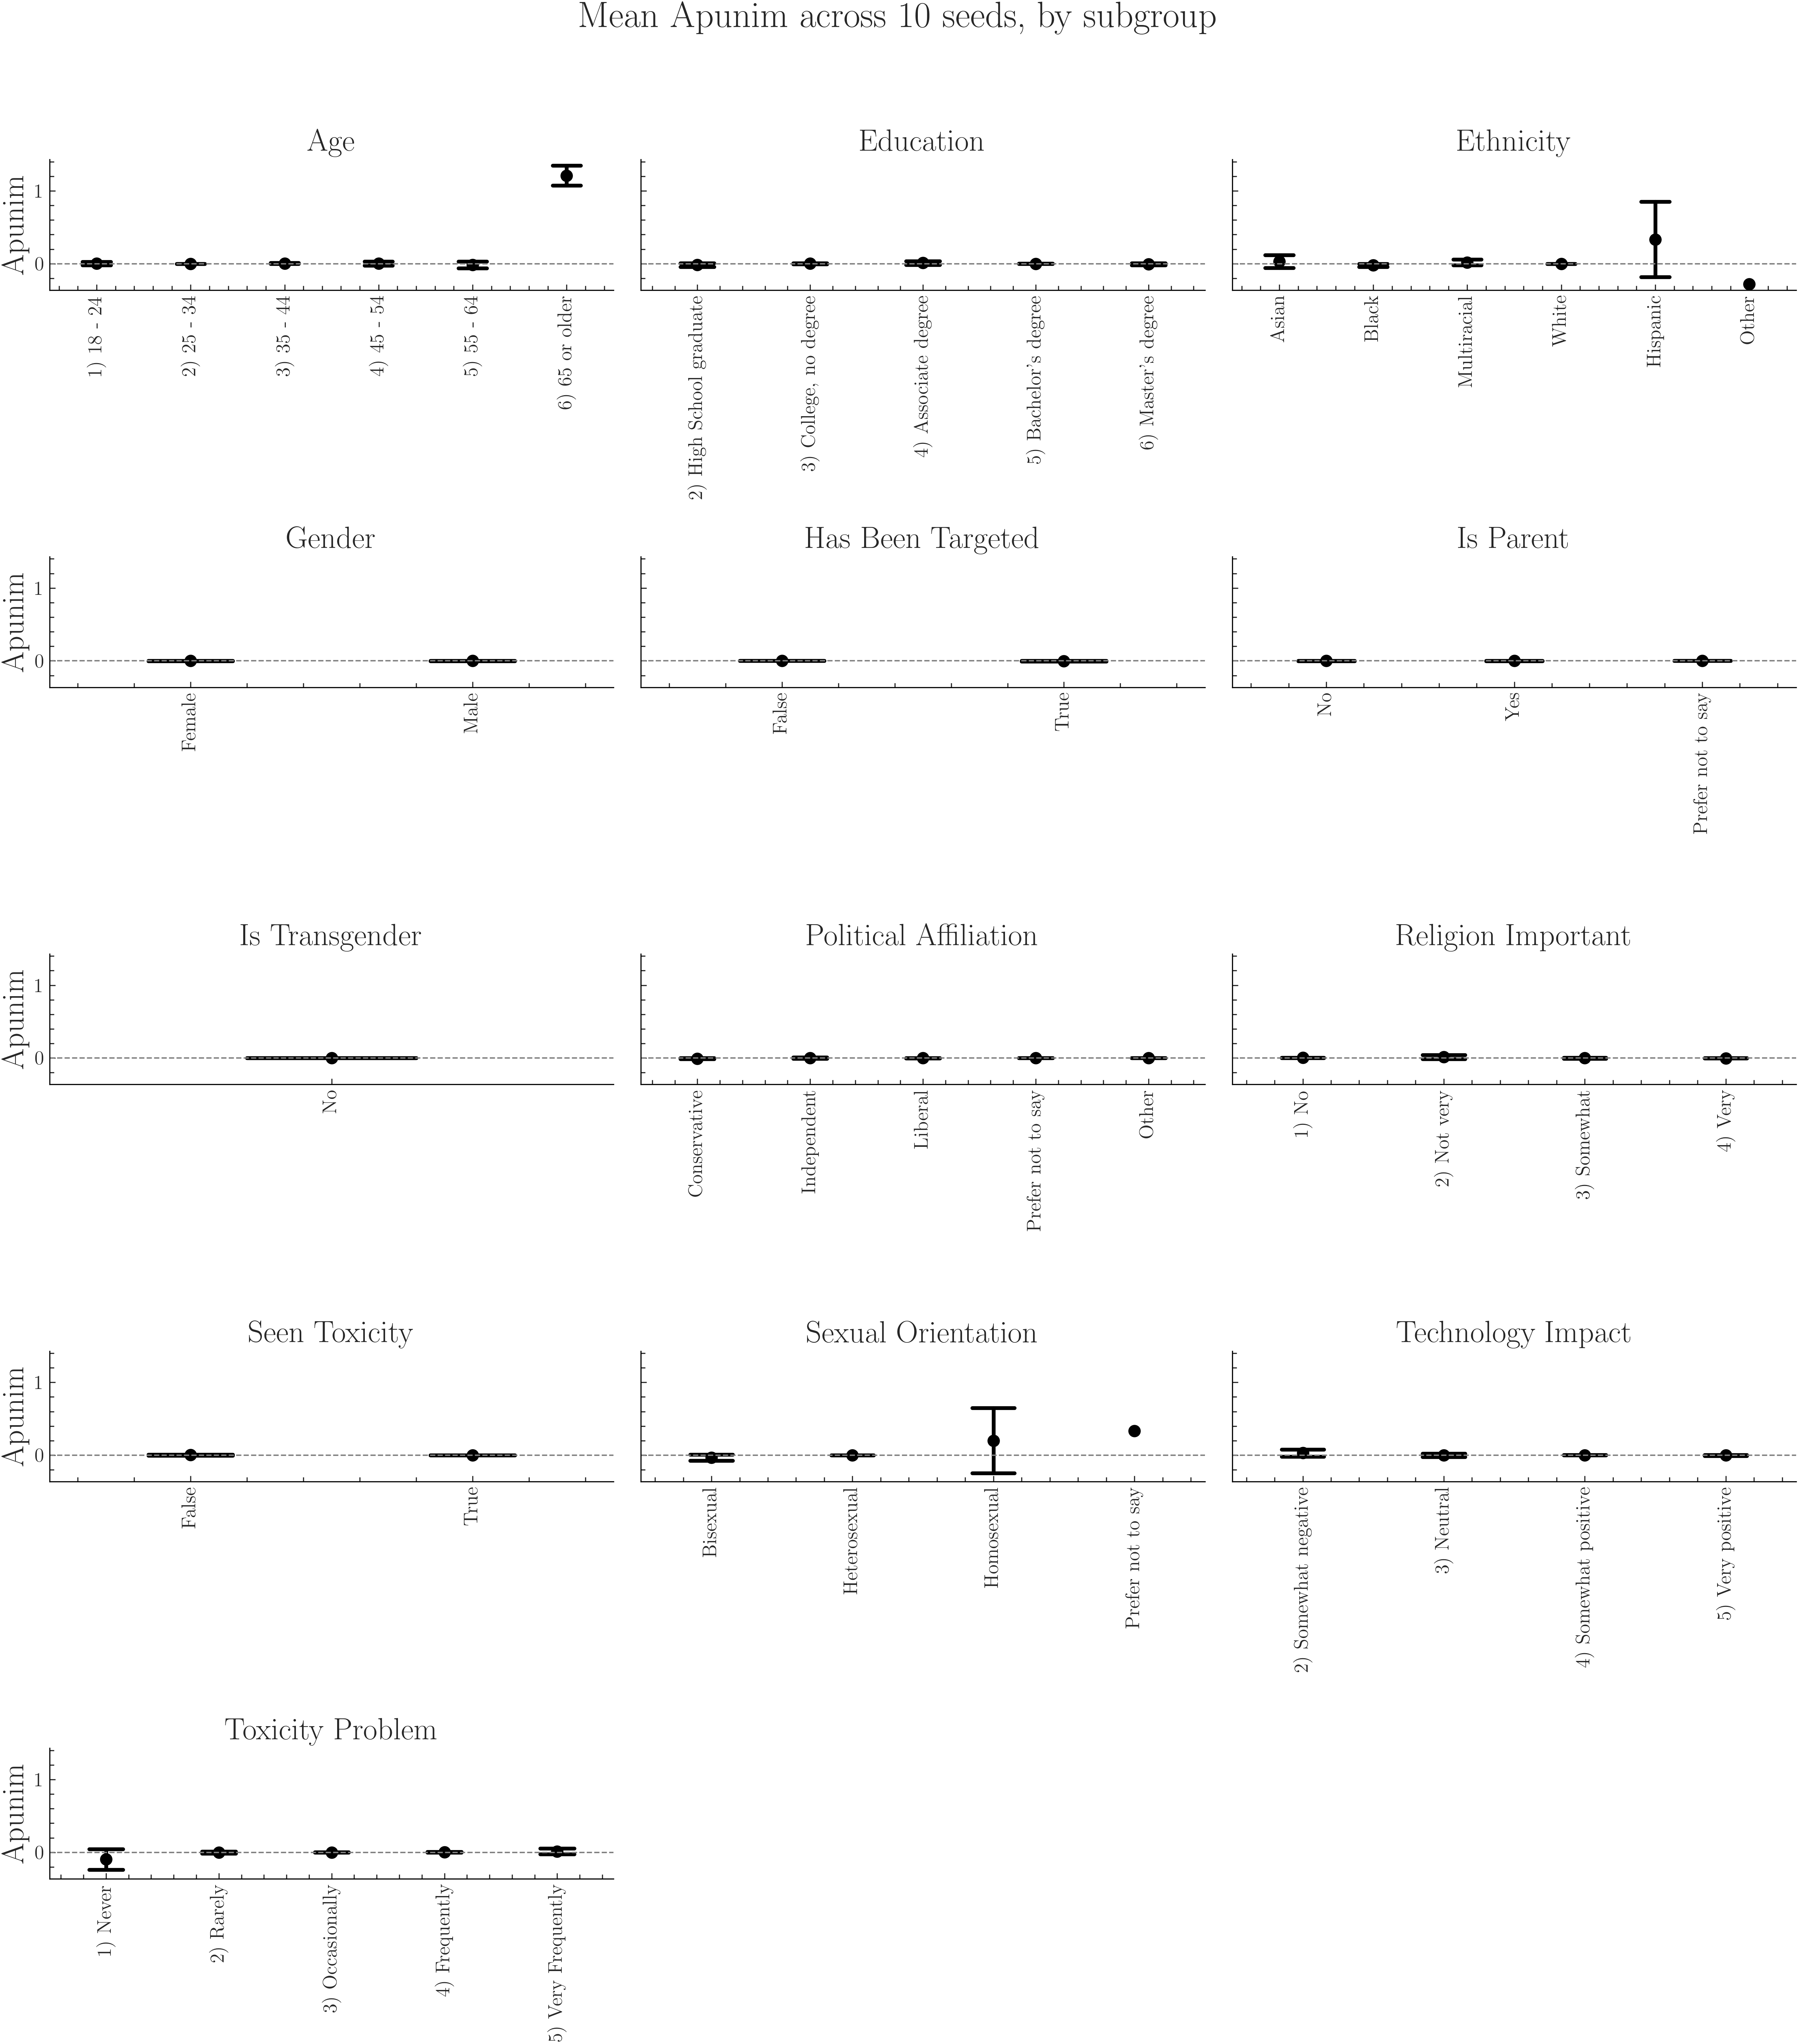
\includegraphics[width=0.55\textwidth]{kumar3k_seed_ablation.png}
	\centering
	\caption{Apunim values on the Kumar dataset ($n_{samples}=3000$) across ten runs with different subsets.  Black bars indicate two \acp{sd}. \ac{pc} dimensions with many groups are more volatile, although all dimensions broadly keep the same apunim sign across subsets.}
	\label{fig:seeds}
\end{figure}

Since our approach was designed for the small-scale datasets common in \ac{nlp}, we were cautious when testing it on the massive Kumar dataset. Because of the data volume, we analyzed various smaller samples (1,000, 10,000, and 30,000 comments), shown in Table~\ref{tab:num-comments-apunim} (rows with more than one N/A values removed). As sample size increased, the statistical metrics (apunim values) consistently shrank, and we found no statistically significant effects in the larger samples.

The test is overly conservative, meaning it almost always suggests there is no significant effect, even when an effect likely exists in reality. This inability to detect a real signal is a Type II Error (a false negative). This suggests that our test is statistically weak or ``underpowered'' in massive settings. Since our methodology is built for the small-scale \ac{nlp} datasets that dominate the research field, we deem this limitation acceptable for the scope of our work. 


\subsection{How does sample section influence apunim?}
\label{app:ablation:samples}

Astute readers may notice that some variability does exist across differently sized samples for the same examined groups, where for example the sign of the apunim value may switch. We note that the statistically significant values (bold rows) change signs only when the apunim value approaches zero in the largest samples. Thus, the results are not inverted, but rather pushed towards zero.

In order to verify that this variability is caused by the sample size, and not by different samples being drawn, we execute a further ablation study. Specifically, we execute the apunim study on the $3000$-sized sample of the dataset, using different subsets of the Kumar dataset. The results can be found in Fig.~\ref{fig:seeds}, where we note that variability is not an issue, except for a couple of cases. These cases seem to represent sparse annotator groups, where missing a few comments may genuinely change the value of the apunim metric. These groups however are largely not detected by apunim as significant either way (see \S\ref{sec:results}).


\section{The ideal subjective dataset}
\label{sec:ideal-dataset}

We briefly discuss the type of data most suited for our proposed methodology, and connect it with current \ac{nlp} datasets.

\paragraph{How many annotators?} Our methodology does not directly require numerous annotators overall, only a sufficient number per item---indeed, statistically significant results can be obtained with as little as four annotations (see Sap-\ac{aa}; Table~\ref{tab:sdb-features}). A large annotator pool however is required to get sufficient coverage on the examined groups. More annotators allow both higher fidelity of each \ac{pc} dimension, and more such dimensions.


\begin{figure}[t]
	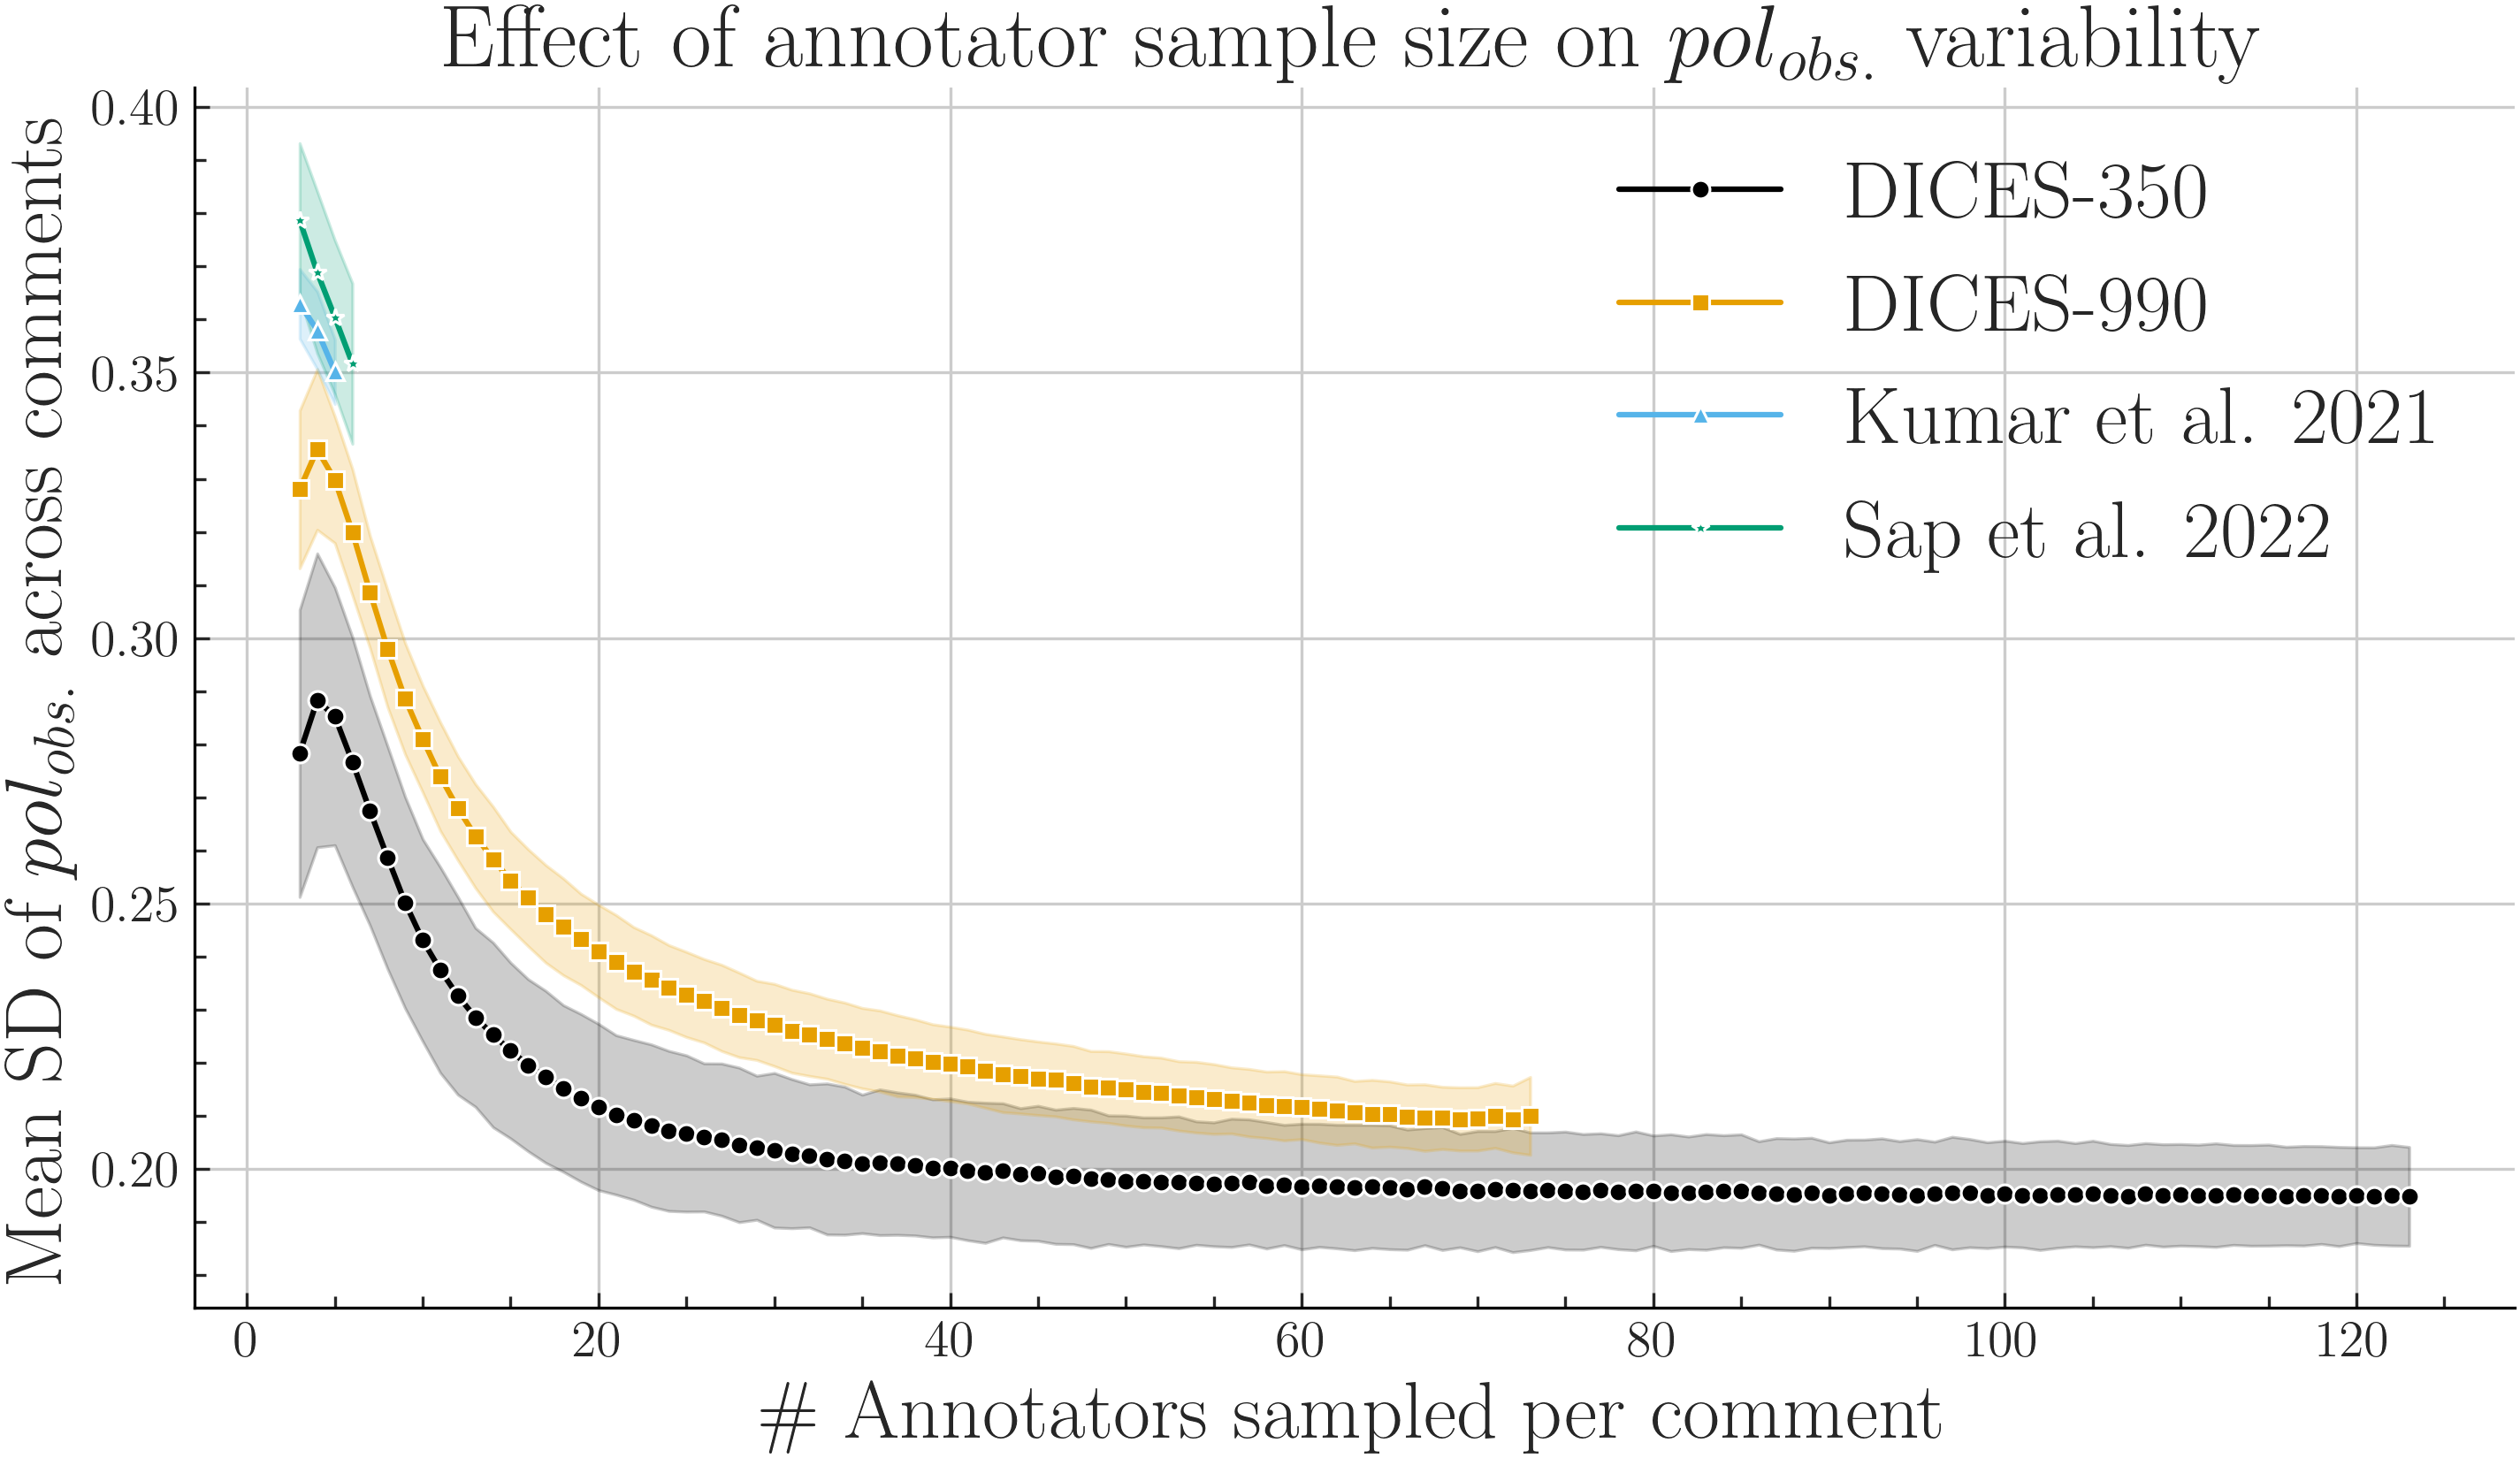
\includegraphics[width=0.55\textwidth]{pol_obs_subsampling_robustness.png}
	\caption{\ac{sd} of $pol_{obs}$ across comments, averaged across $1000$ runs (Eq.~\ref{eq:observed}). Shaded areas represent two \acp{sd}. Pol. estimates benefit from more annotators up to $n=20$, at which point they begin to plateau.}
	\label{fig:std_error}
\end{figure}

\paragraph{How many annotators per item?} We investigate observed polarization against varying numbers of annotators. Specifically, for every comment, we repeatedly sampled $n$ annotators with replacement, calculated $pol_{obs}$ for each sample and measured \ac{sd}, averaging it across 1000 same-sized samples. As shown in Fig.~\ref{fig:std_error}, $pol_{obs}$ exhibits a clear, inverse relationship with the number of annotators, attributed to better histogram estimation provided by \ac{ndfu} (\S\ref{sec:apunim:group-vs-global}), though the rate of gain substantially diminishes after 20 annotators. Interestingly, some variability persists even with a very high annotator count.

\paragraph{How many items?} Our methodology is designed to work with smaller datasets common in \ac{nlp}. Three of the four datasets in the study feature low (300--600) item counts, while the Kumar dataset has been subsampled to 3\% of its original size. Large datasets should be used only to provide larger coverage on the target domain, since a much better representation of individual groups can be achieved with more annotators per item, rather than more items. Smaller datasets may also be more practical for social science analysis~\cite{rossi_2024}.

\section{Full results}
\label{app:full}

\begin{figure}[ht]
	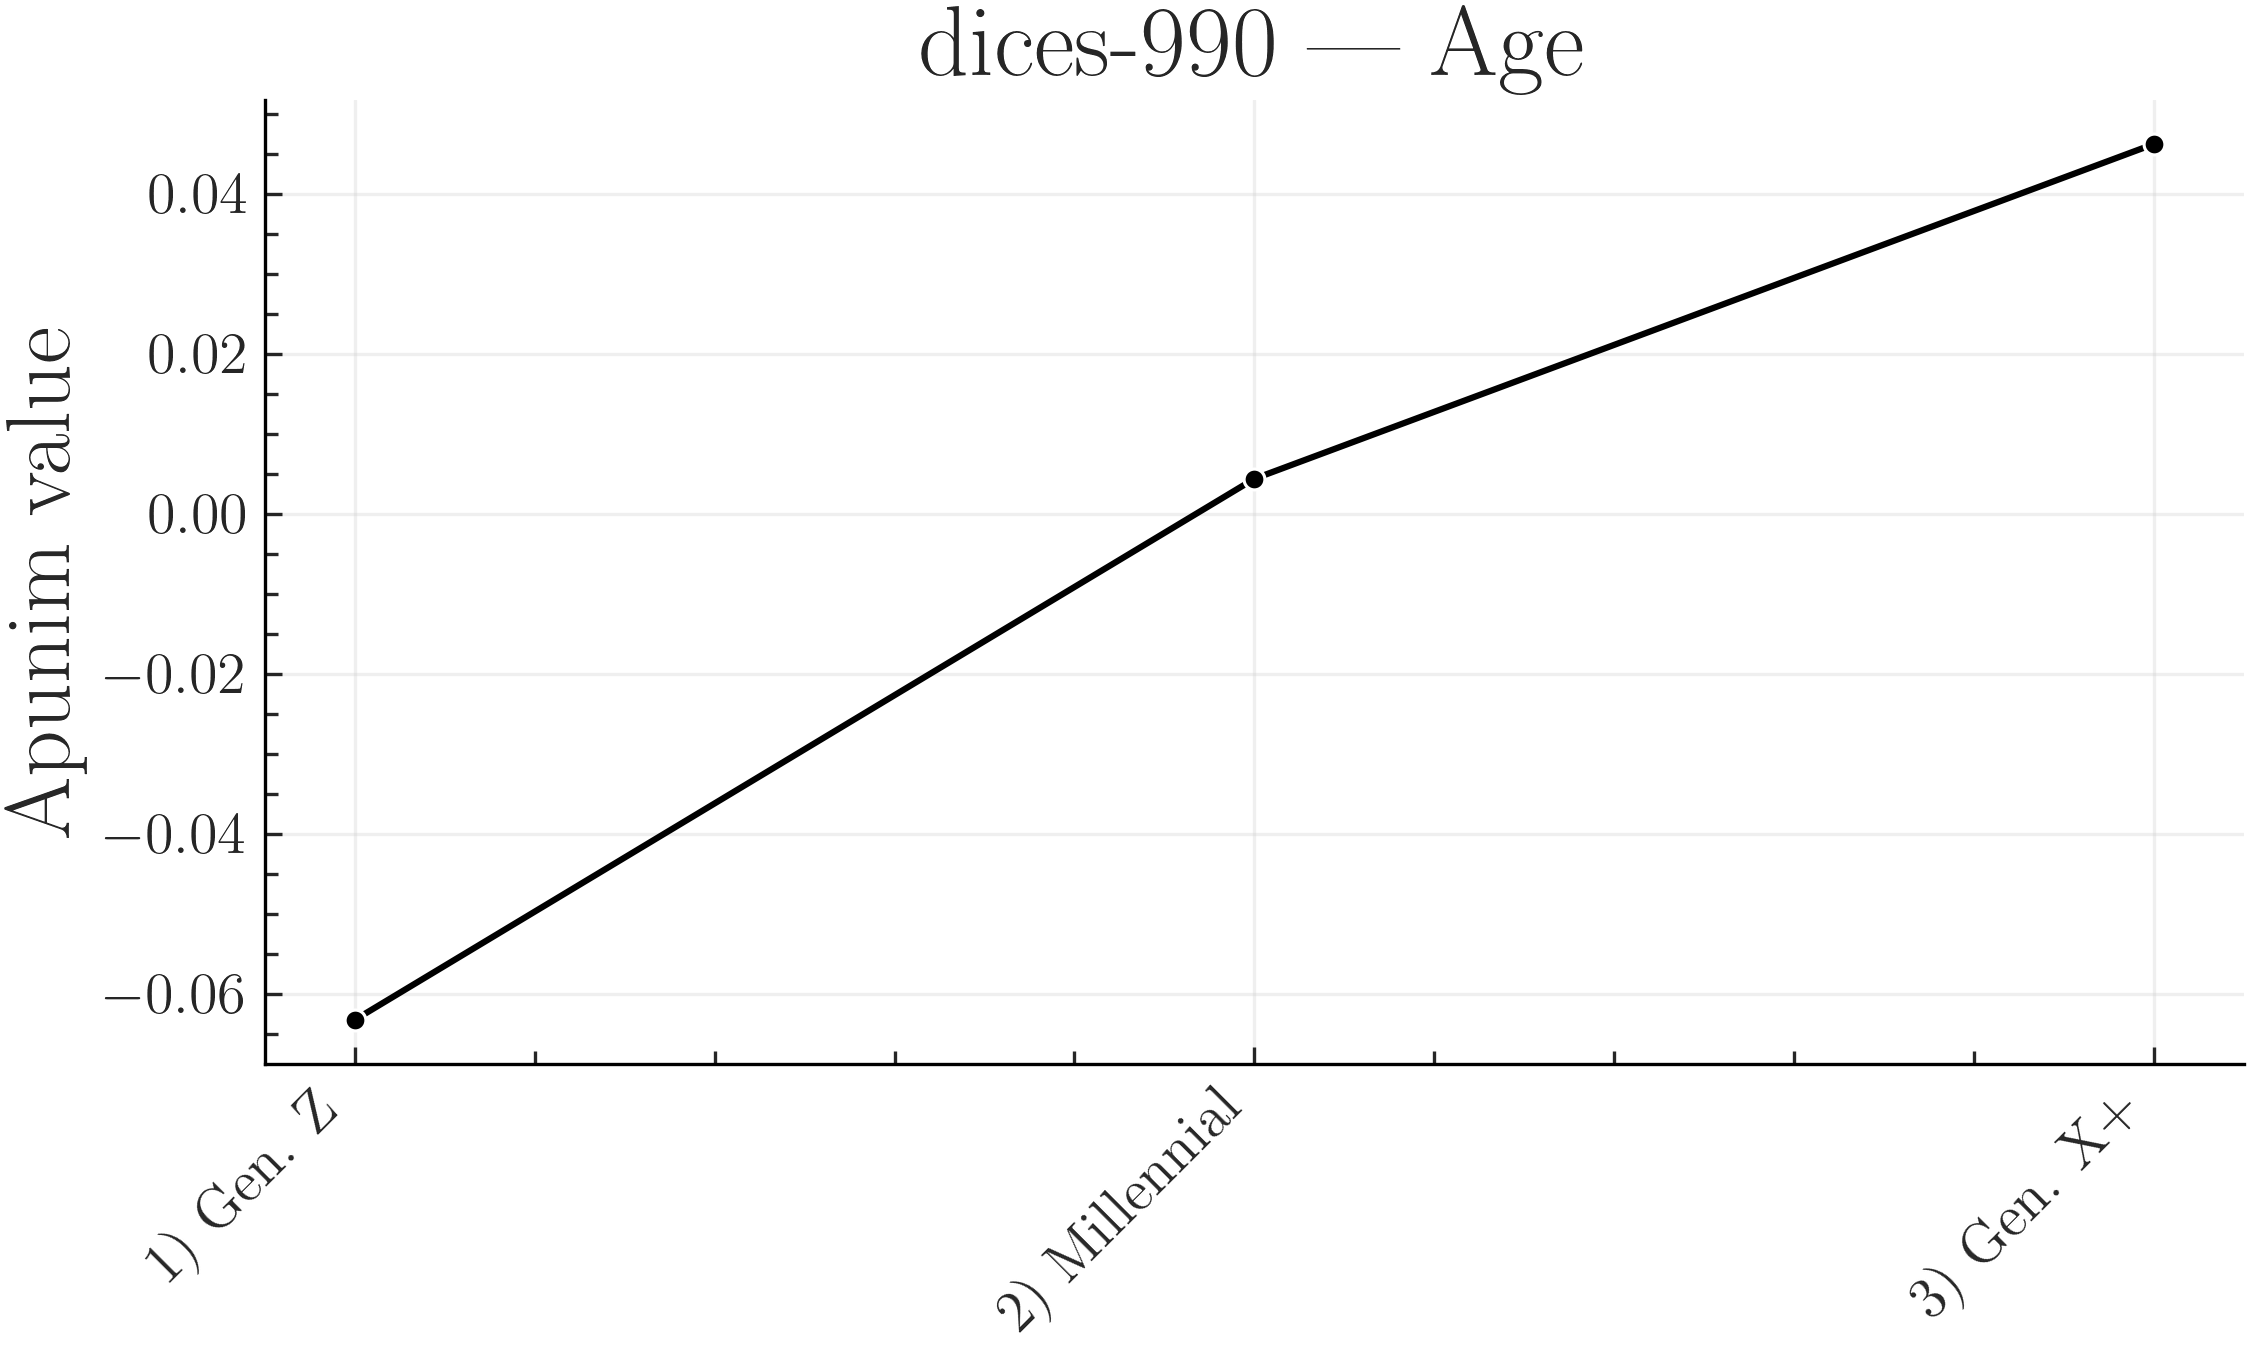
\includegraphics[width=0.48\textwidth]{apunim_ordinal_dices-990_Age.png}
	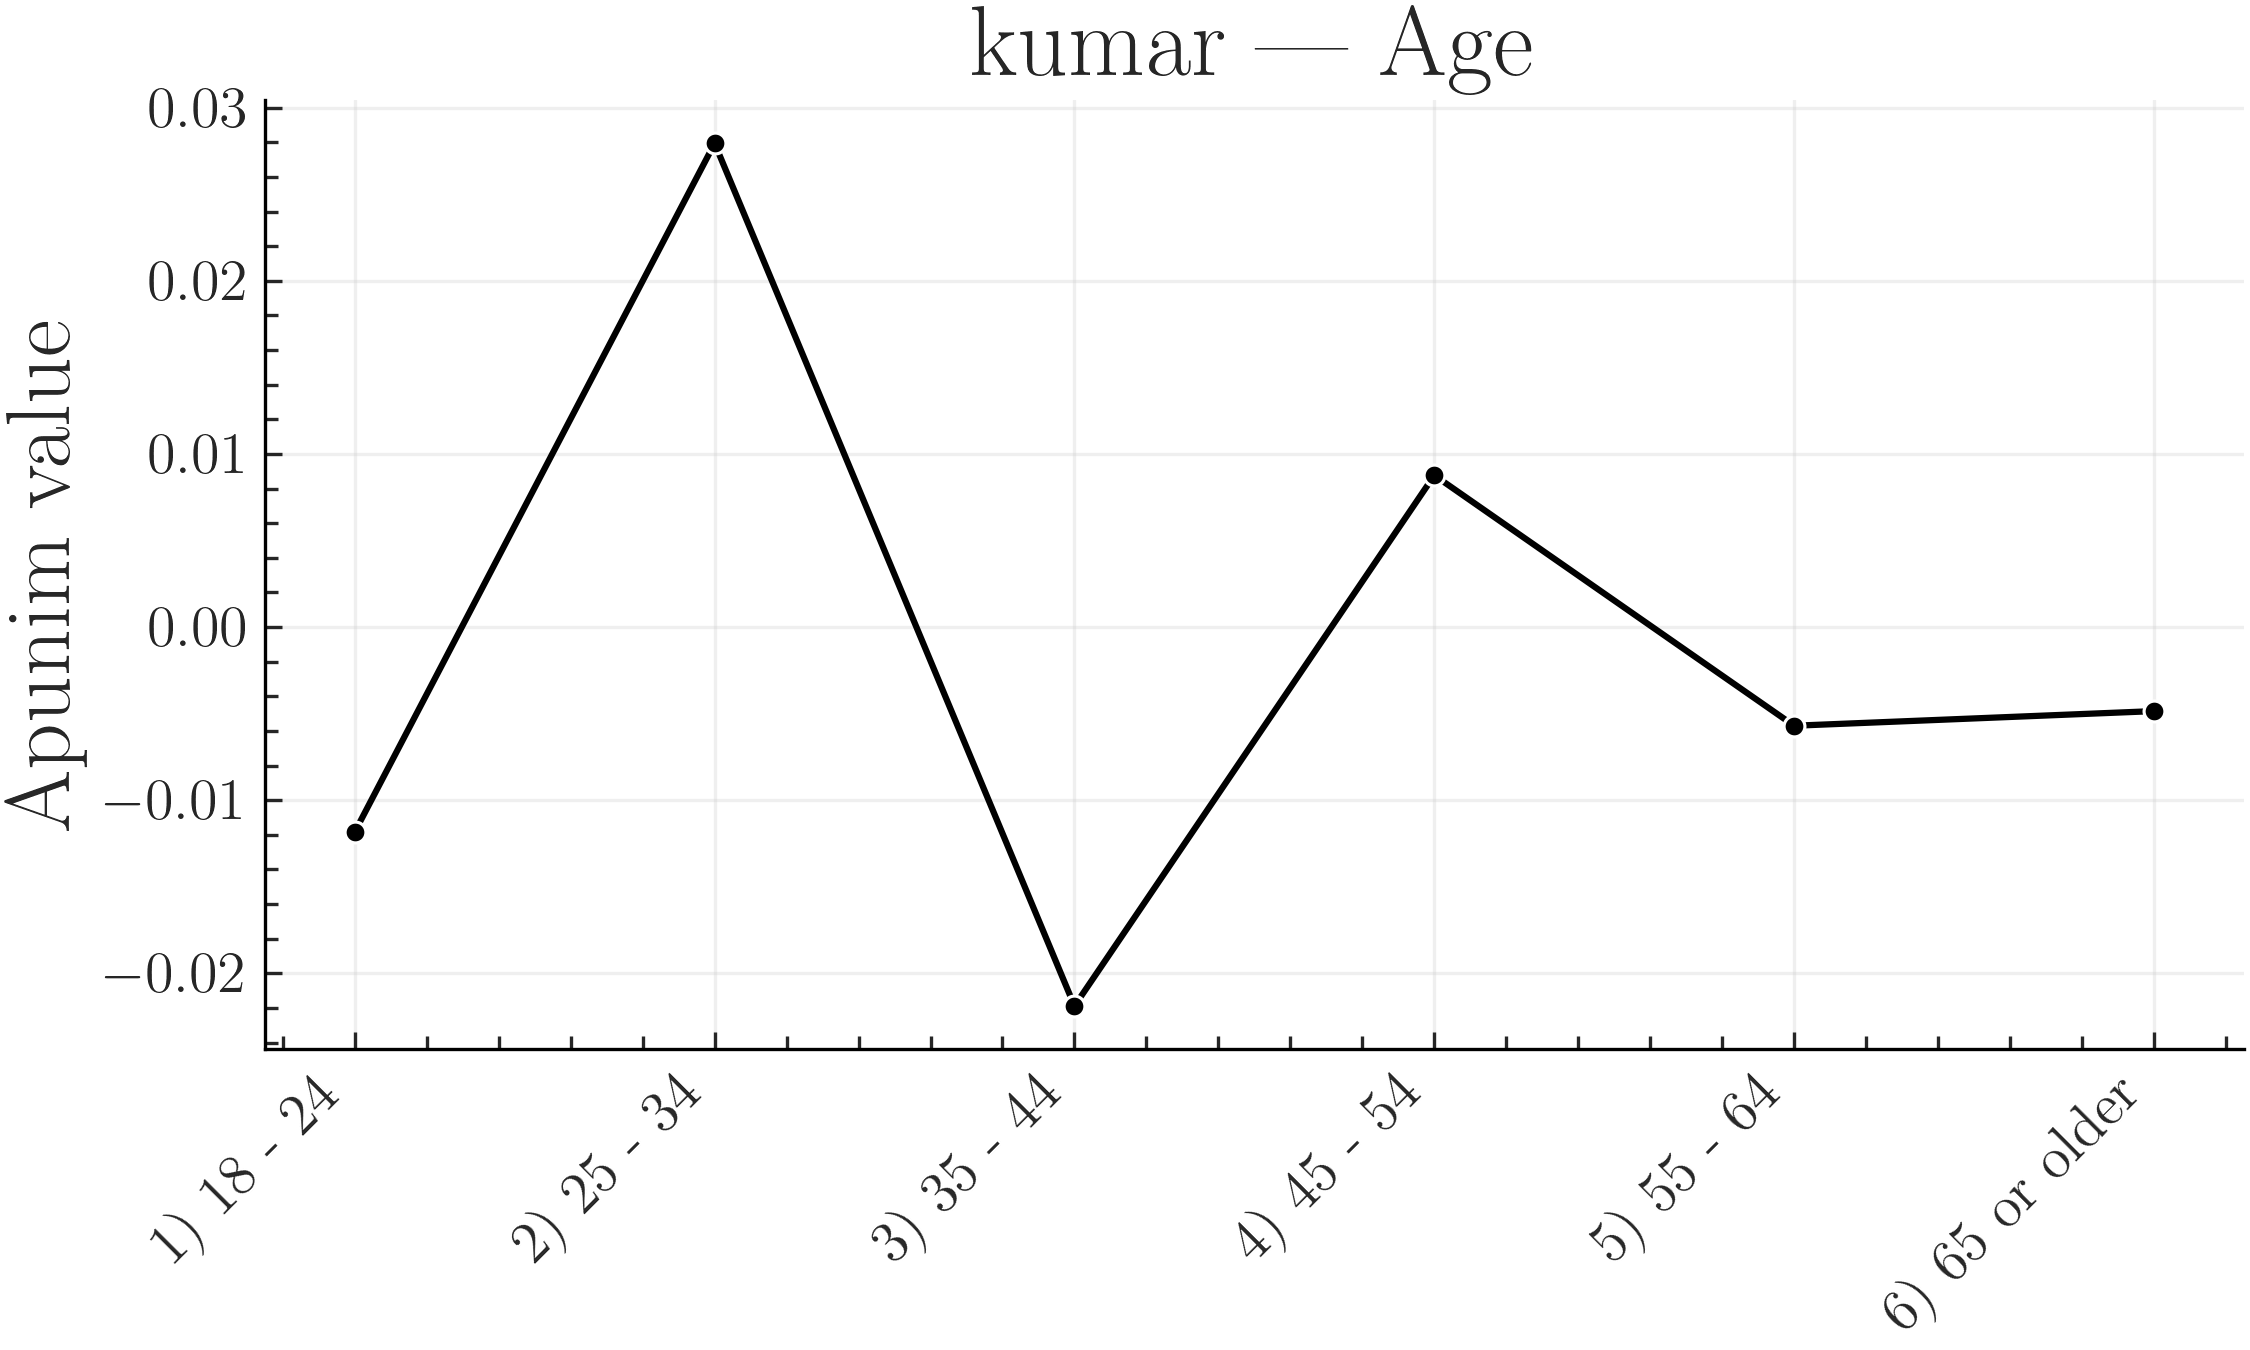
\includegraphics[width=0.48\textwidth]{apunim_ordinal_kumar_Age.png}
	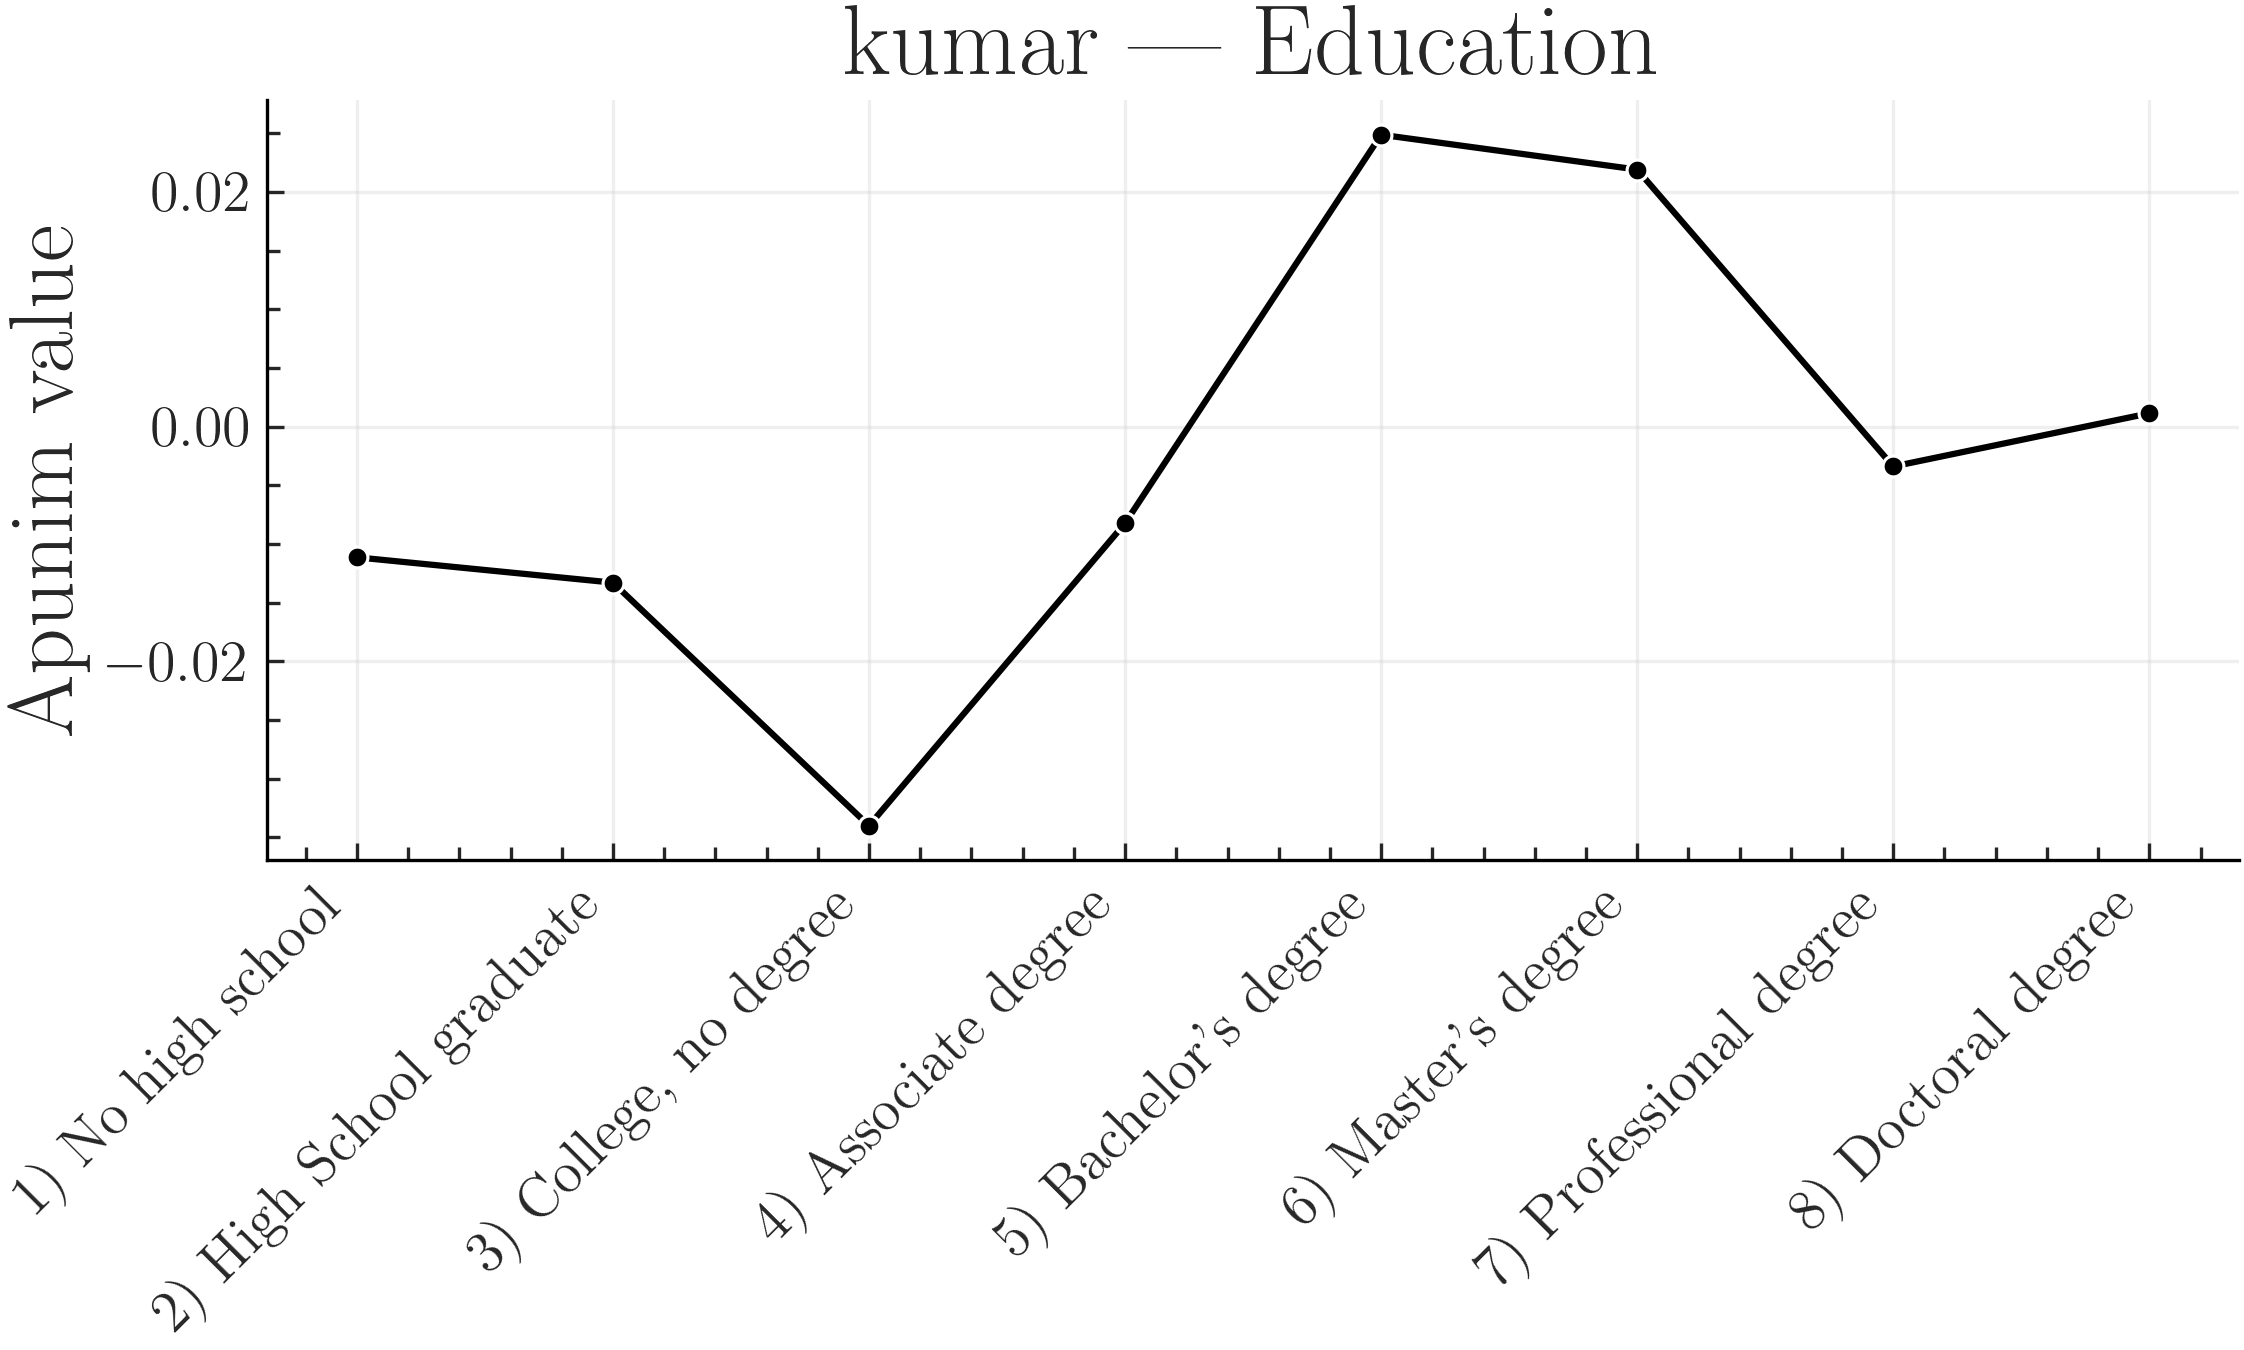
\includegraphics[width=0.48\textwidth]{apunim_ordinal_kumar_Education.png}
	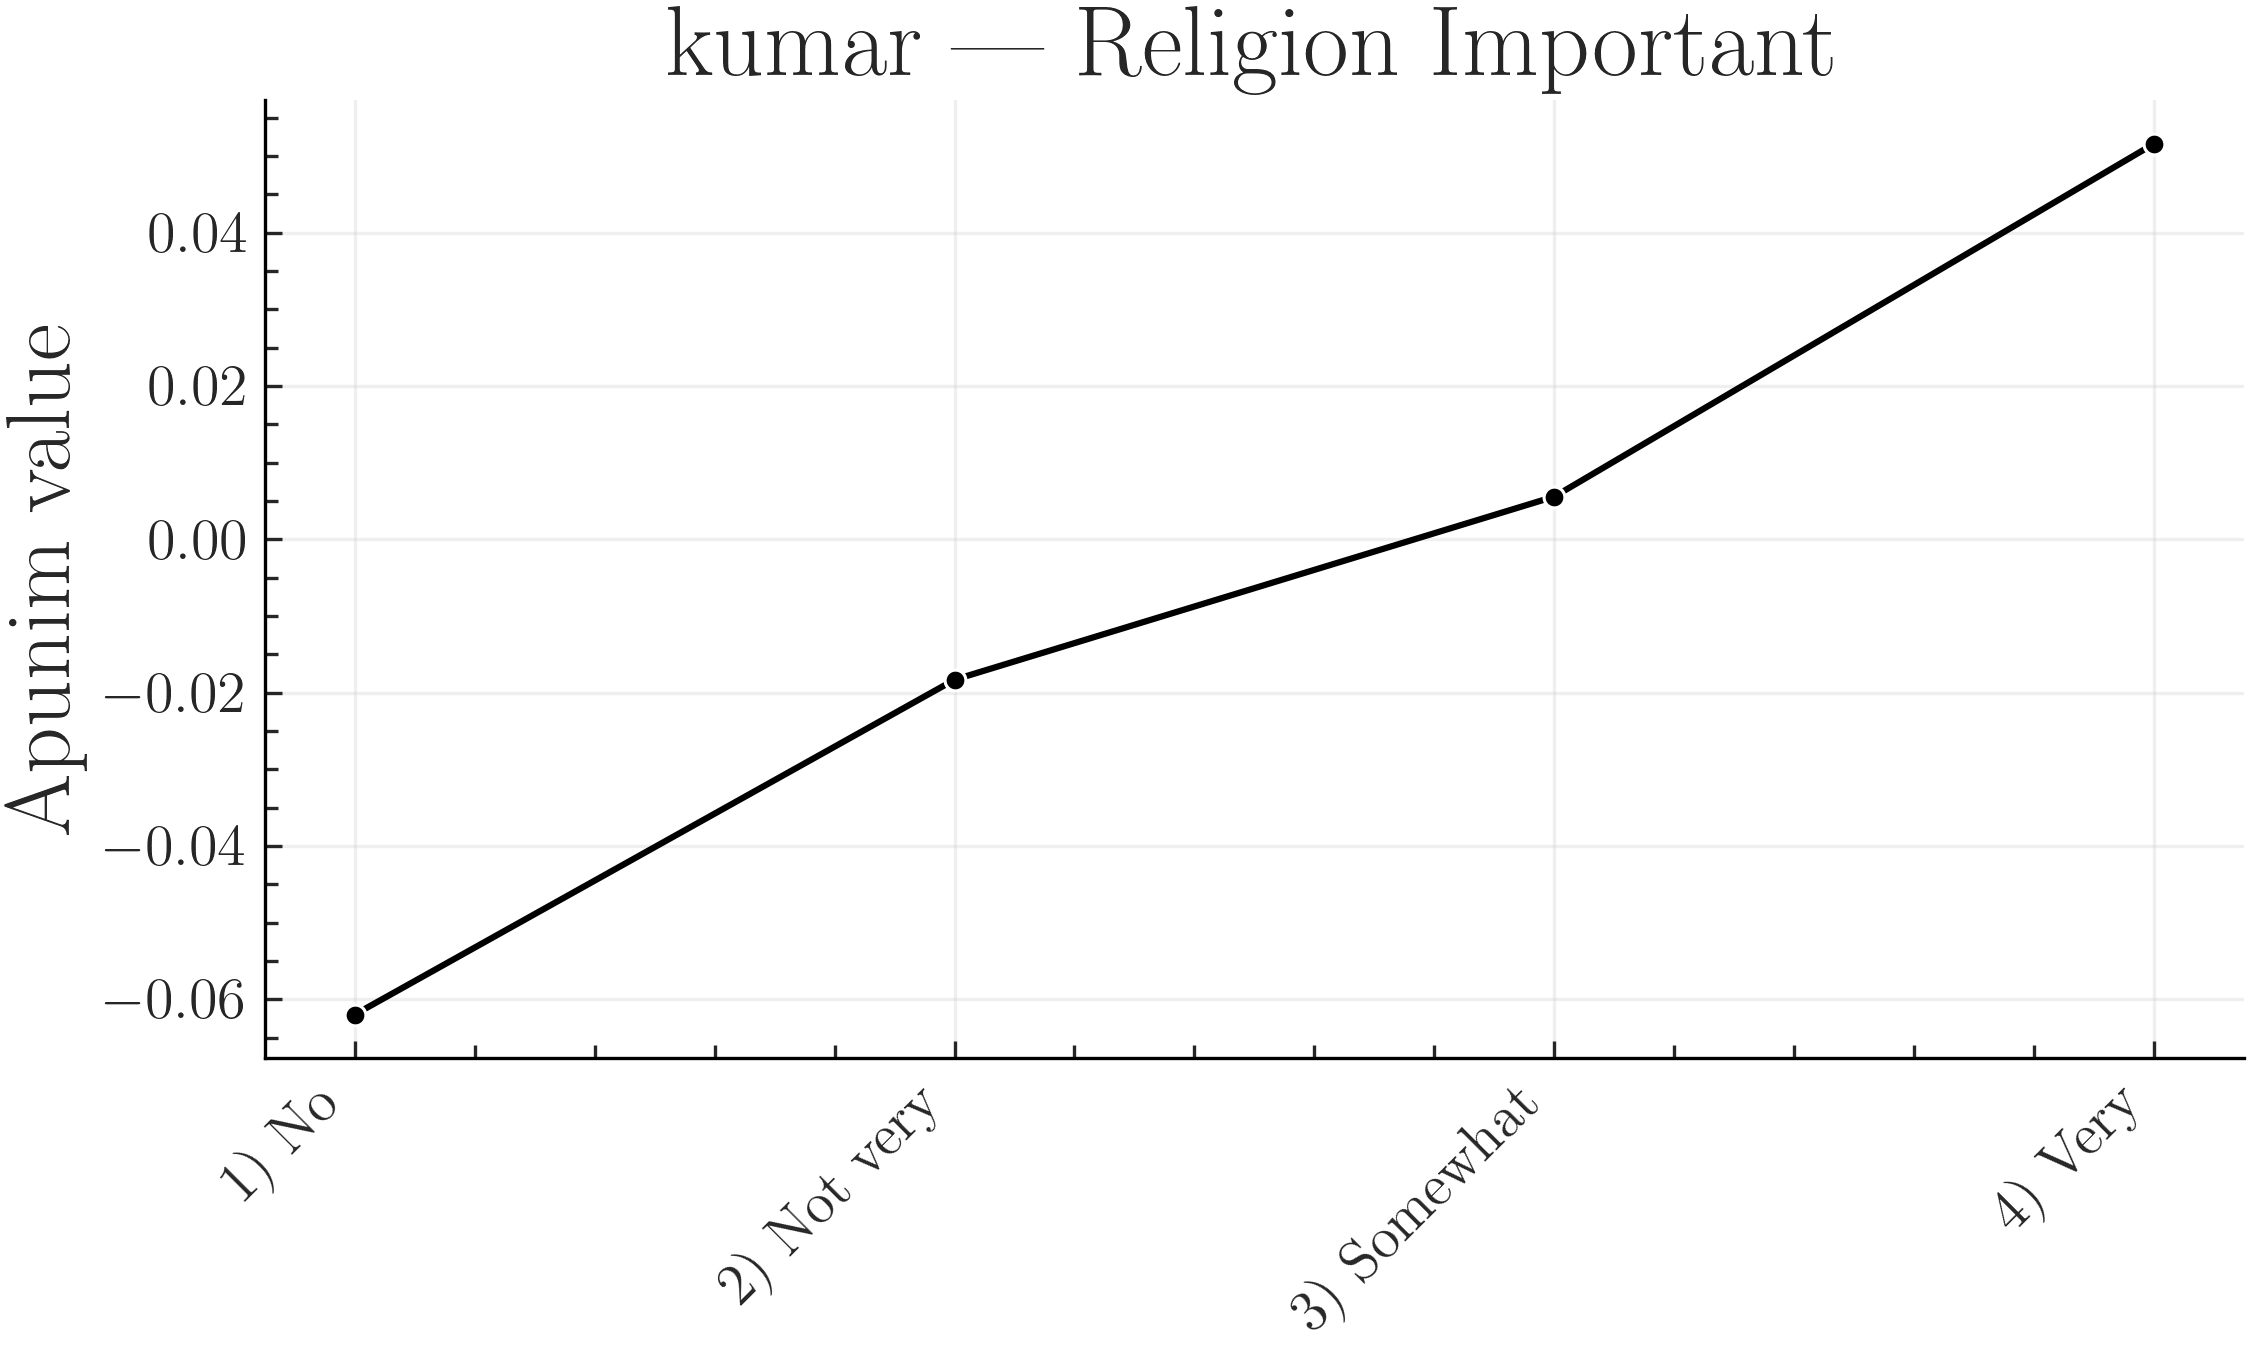
\includegraphics[width=0.48\textwidth]{apunim_ordinal_kumar_Religion_Important.png}
	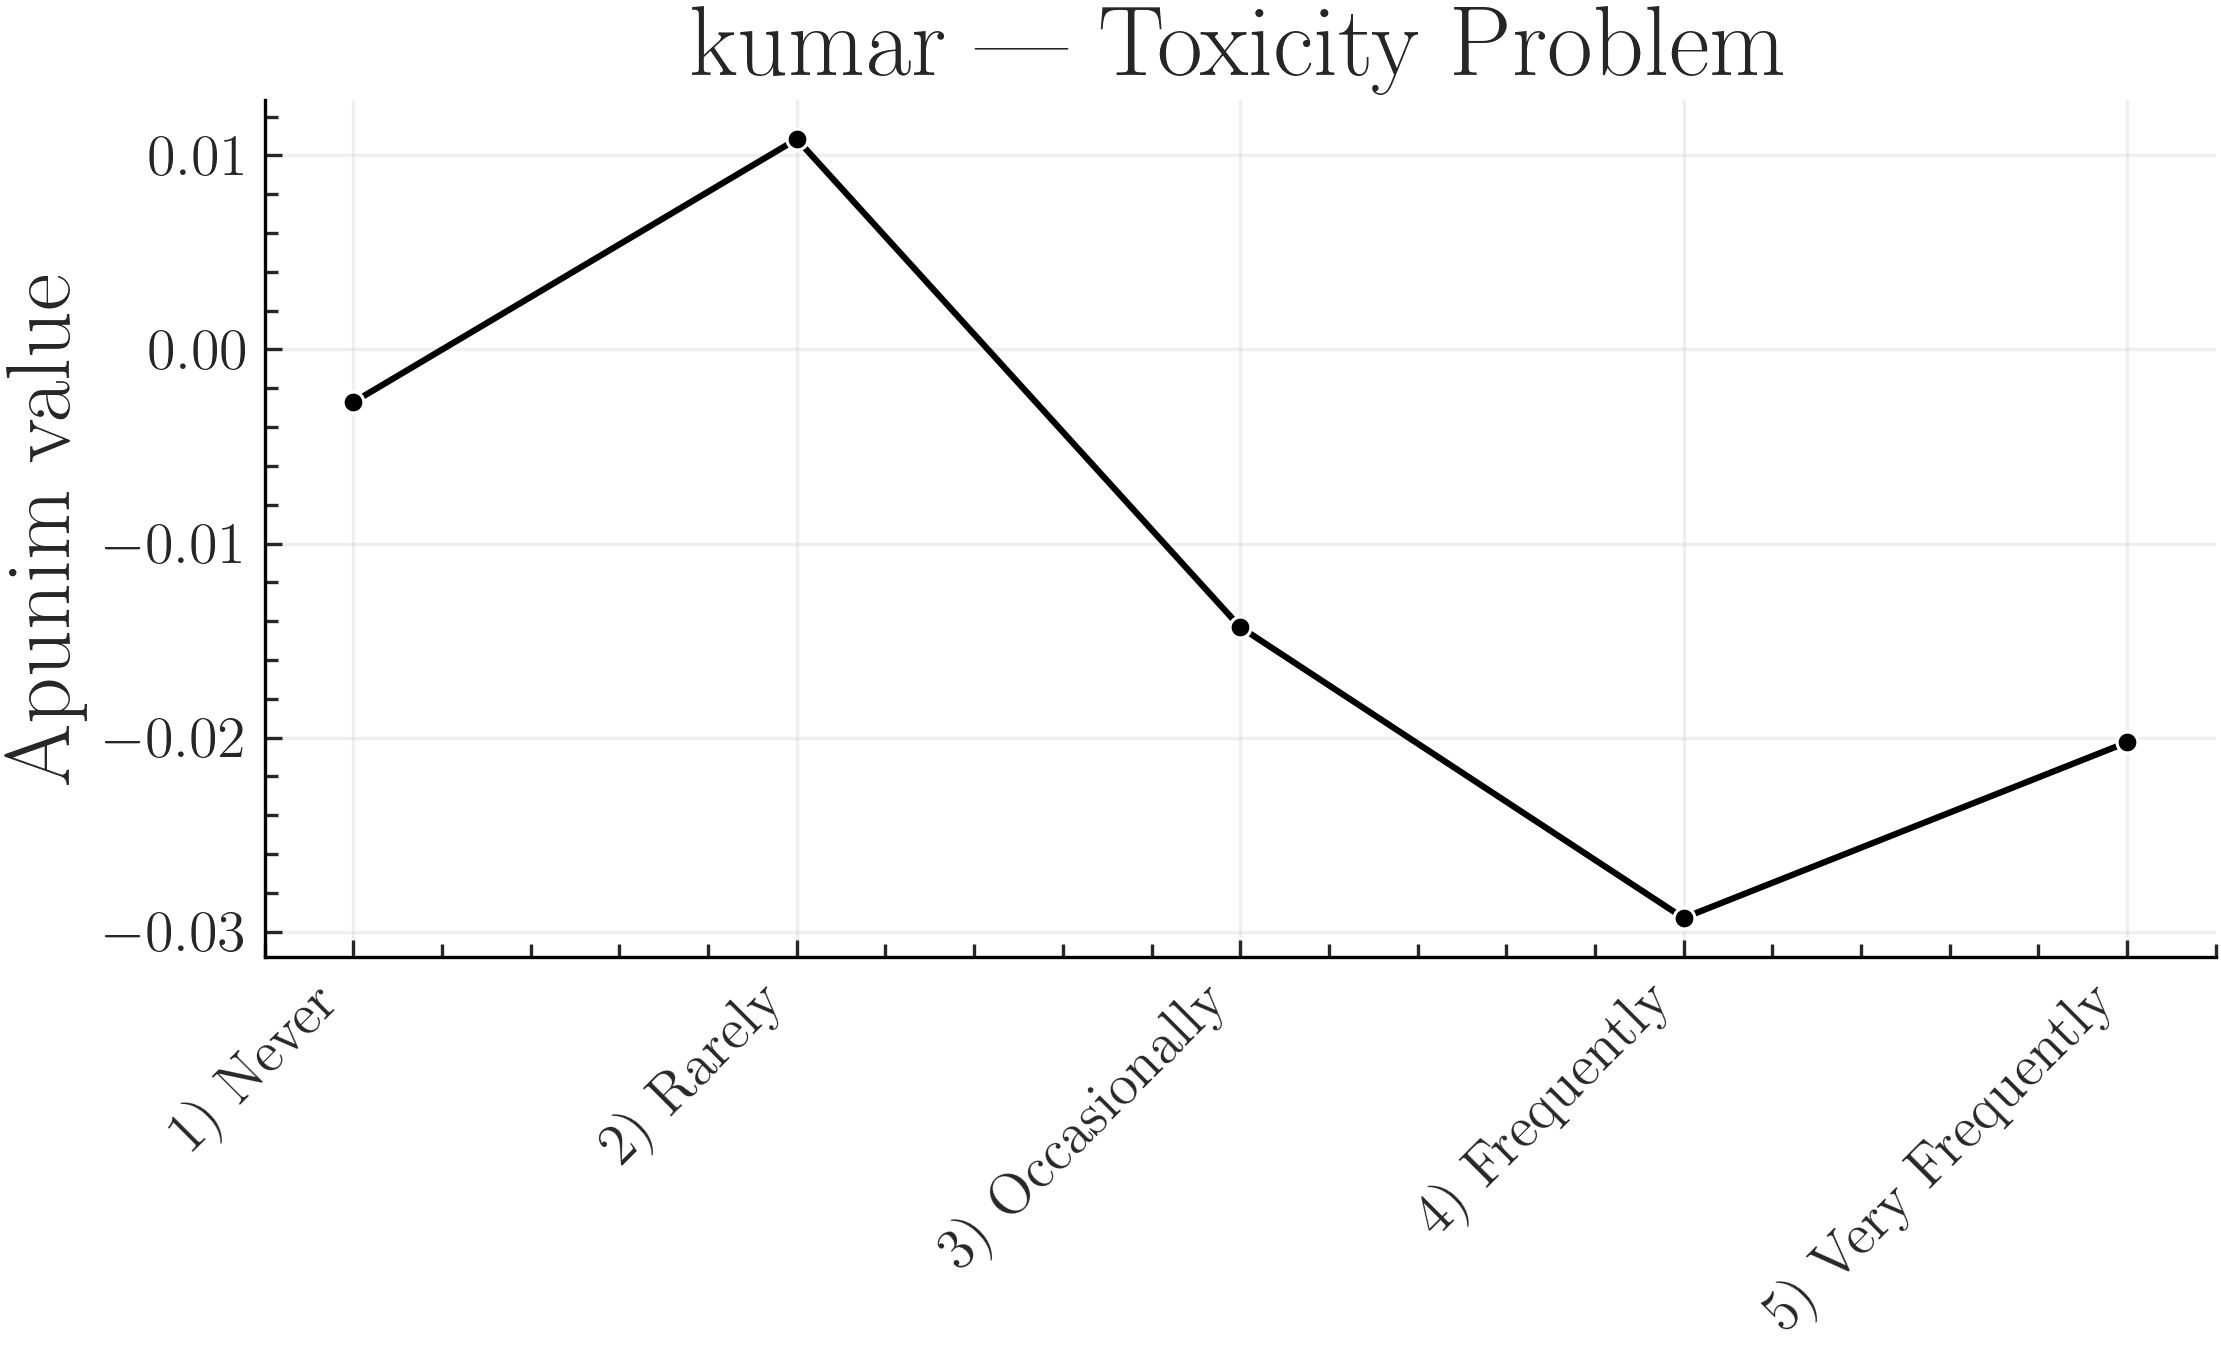
\includegraphics[width=0.48\textwidth]{apunim_ordinal_kumar_Toxicity_Problem.png}
	\caption{Apunim values expanded for each ordinal \ac{pc} dimension. This figure is complementary to Fig.~\ref{fig:ordinal}. The values in the graphs were extracted from the Tables of App.~\ref{app:full}. }
	\label{fig:ordinal-full}
\end{figure}

\begin{table}[t]
	\centering
	\scriptsize 
	\begin{tabularx}{\columnwidth}{X r r r}
		\toprule
		\textbf{Group} & \textbf{apunim} & \textbf{pvalue} & \textbf{support} \\
		\midrule
		
		\multicolumn{4}{c}{\textbf{Kumar}} \\
		\midrule
		\rowcolor{gray!15}
		Age=18-24 & -.0118 & .4822 & 1431 \\
		Age=25-34 & .0279 & .1185 & 4888 \\
		\rowcolor{gray!15}
		Age=35-44 & -.0219 & .1733 & 3102 \\
		Age=45-54 & .0088 & .5394 & 1668 \\
		\rowcolor{gray!15}
		Age=55-64 & -.0057 & .6592 & 938 \\
		\rowcolor{gray!15}
		Age=65 or older & -.0049 & .6747 & 409 \\
		Age=N/A & .0000 & N/A & 37 \\
		Age=Under 18 & .0000 & N/A & 2 \\
		\rowcolor{gray!15}
		Ed=No HS & -.0111 & .5278 & 60 \\
		\rowcolor{gray!15}
		Ed=High School & -.0133 & .3461 & 1123 \\
		Ed=College & -.0340 & .0189 & 2508 \\
		\rowcolor{gray!15}
		Ed=Associate & -.0082 & .5963 & 1362 \\
		Ed=Bachelor's & .0249 & .1091 & 5007 \\
		Ed=Master's & .0219 & .1091 & 1982 \\
		\rowcolor{gray!15}
		Ed=Professional & -.0034 & .7459 & 192 \\
		Ed=Doctoral & .0011 & .8651 & 164 \\
		Ed=Other & .0000 & N/A & 28 \\
		Ed=N/A & .0000 & N/A & 63 \\
		\rowcolor{gray!15}
		Eth=Asian & -.0019 & .9332 & 720 \\
		Eth=Black & .0143 & .7070 & 1671 \\
		\rowcolor{gray!15}
		Eth=Hispanic & -.0075 & .9092 & 352 \\
		\rowcolor{gray!15}
		Eth=Multiracial & -.0026 & .9332 & 540 \\
		\rowcolor{gray!15}
		Eth=Other & -.0007 & .9332 & 204 \\
		\rowcolor{gray!15}
		Eth=Unknown & -.0063 & .9092 & 189 \\
		\rowcolor{gray!15}
		Eth=White & -.0291 & .0416 & 6619 \\
		\rowcolor{gray!15}
		Gen=Female & -.0245 & .0720 & 6141 \\
		Gen=Male & .0261 & .0720 & 5479 \\
		\rowcolor{gray!15}
		Gen=Nonbinary & -.0014 & .9436 & 81 \\
		\rowcolor{gray!15}
		Gen=Unknown & -.0008 & .9436 & 104 \\
		\rowcolor{gray!15}
		Targeted=False & -.0482 & 1.04e-05 & 6632 \\
		Targeted=True & .0146 & .2310 & 3643 \\
		\rowcolor{gray!15}
		IsParent=No & -.0686 & 2.39e-08 & 5514 \\
		IsParent=N/A & .0017 & .8913 & 130 \\
		IsParent=Yes & .0490 & 2.85e-05 & 6216 \\
		\rowcolor{gray!15}
		IsTrans=No & -.0788 & 7.47e-05 & 1697 \\
		\rowcolor{gray!15}
		IsTrans=N/A & -.0007 & .9483 & 128 \\
		\rowcolor{gray!15}
		IsTrans=Yes & -.0073 & .7711 & 340 \\
		
		Pol=Conservative & .0269 & .0534 & 3386 \\
		\rowcolor{gray!15}
		Pol=Independent & -.0201 & .1371 & 3432 \\
		\rowcolor{gray!15}
		Pol=Liberal & -.0278 & .0534 & 4945 \\
		\rowcolor{gray!15}
		Pol=Other & -.0132 & .2947 & 271 \\
		Pol=N/A & .0034 & .6523 & 511 \\
		\rowcolor{gray!15}
		RelImp=No & -.0620 & 2.96e-07 & 3864 \\
		\rowcolor{gray!15}
		RelImp=Not very & -.0183 & .1039 & 1493 \\
		Ed=Somewhat & .0056 & .6169 & 3012 \\
		RelImp=Very & .0516 & 4.58e-05 & 4062 \\
		RelImp=N/A & .0066 & .2968 & 194 \\
		
		SeenTox=False & .0350 & .0029 & 3050 \\
		\rowcolor{gray!15}
		SeenTox=True & -.0766 & 4.82e-13 & 6360 \\
		
		SexOrient=Bisexual & .0087 & .7884 & 1481 \\
		\rowcolor{gray!15}
		SexOrient=Heterosexual & -.0500 & 3.22e-05 & 5721 \\
		\rowcolor{gray!15}
		SexOrient=Homosexual & -.0048 & .7884 & 430 \\
		SexOrient=Other & .0009 & .9055 & 115 \\
		\rowcolor{gray!15}
		SexOrient=N/A & -.0061 & .7884 & 265 \\
		
		TechImp=Very neg & .0000 & N/A & 118 \\
		\rowcolor{gray!15}
		TechImp=Somewhat neg & -.0085 & .4097 & 1179 \\
		TechImp=Neutral & .0085 & .4097 & 1603 \\
		\rowcolor{gray!15}
		TechImp=Somewhat & -.0285 & .0691 & 6040 \\
		TechImp=Very pos& .0105 & .4097 & 3315 \\
		\rowcolor{gray!15}
		ToxProblem=Never & -.0027 & .8071 & 741 \\
		ToxProblem=Rarely & .0108 & .3965 & 2087 \\
		\rowcolor{gray!15}
		ToxProblem=Occ & -.0143 & .3809 & 4347 \\
		\rowcolor{gray!15}
		ToxProblem=Freq & -.0293 & .0507 & 3740 \\
		\rowcolor{gray!15}
		ToxProblem=Very & -.0202 & .1404 & 1625 \\
		
		\bottomrule
	\end{tabularx}
	\caption{Apunim results for the Kumar dataset. $^{*}$ denotes $p<0.10$, $^{**}$ denotes $p<0.05$, and $^{***}$ denotes $p<0.01$. Rows shaded in gray indicate a negative $\text{apunim}$ value.}
	\label{tab:sdb-features}
\end{table}

\begin{table}[t]
	\small
	\centering
	
	\begin{tabularx}{\columnwidth}{X r r r}
		\toprule
		\textbf{Group} & \textbf{apunim} & \textbf{pvalue} & \textbf{support} \\
		\midrule
		
		\multicolumn{4}{c}{\textbf{Sap}} \\
		\midrule
		\rowcolor{gray!15}
		Age=GenX+ & -.066 & .708 & 271 \\
		Age=Millennial & .007 & .744 & 1886 \\
		Ethnicity=black & .042 & 4.000 & 4 \\
		\rowcolor{gray!15}
		Ethnicity=white & -.000 & .998 & 1896 \\
		\rowcolor{gray!15}
		Gender=Man & -.091 & .000 & 1439 \\
		Gender=Woman & .244 & .000 & 877 \\
		
		\bottomrule
	\end{tabularx}
	\caption{Apunim results for the Sap Dataset. $^{*}$ denotes $p<0.10$, $^{**}$ denotes $p<0.05$, and $^{***}$ denotes $p<0.01$.  Rows shaded in gray indicate a negative $\text{apunim}$ value. Groups for which no polarized comments among groups not included.}
	\label{tab:sap-full}
\end{table}

\begin{table}[t]
	\centering
	\small 
	\begin{tabularx}{\columnwidth}{X r r r}
		\toprule
		\textbf{Group} & \textbf{apunim} & \textbf{pvalue} & \textbf{support} \\
		\midrule
		
		\multicolumn{4}{c}{\textbf{DICES-350}} \\
		\midrule
		
		Age Gen. Z & .007 & .539 & 17528 \\
		Age Millennial & .006 & .539 & 11268 \\
		\rowcolor{gray!15}
		Age Gen. X+ & -.019 & .166 & 9703 \\
		\rowcolor{gray!15}
		Ed=College + & -.012 & .234 & 23475 \\
		\rowcolor{gray!15}
		Ed=High school & -.015 & .186 & 12833 \\
		Ed=Other & .021 & .025 & 2191 \\
		Gender Man & .019 & .058 & 19093 \\
		\rowcolor{gray!15}
		Gender Woman & -.021 & .058 & 19406 \\
		Race African Am. & .043 & 2.41e-05 & 9077 \\
		\rowcolor{gray!15}
		Race Asian & -.066 & 1.16e-10 & 8138 \\
		Race Latino & .003 & .920 & 6886 \\
		Race Multiracial & .000 & .980 & 5008 \\
		Race White & .020 & .067 & 9390 \\
		\bottomrule
	\end{tabularx}
	\caption{Apunim results for the DICES-350 Dataset. $^{*}$ denotes $p<0.10$, $^{**}$ denotes $p<0.05$, and $^{***}$ denotes $p<0.01$.  Rows shaded in gray indicate a negative $\text{apunim}$ value. Groups for which no polarized comments among groups not included.}
	\label{tab:dices350-full}
\end{table}

\begin{table}[t]
	\centering
	\small 
	\begin{tabularx}{\columnwidth}{X r r r}
		\toprule
		\textbf{Group} & \textbf{apunim} & \textbf{pvalue} & \textbf{support} \\
		\midrule
		
		\multicolumn{4}{c}{\textbf{DICES-990}} \\
		\midrule
		\rowcolor{gray!15}
		Age Gen. Z & -.063 & 3.05e-25 & 13741 \\
		Age Millennial & .004 & .495 & 38436 \\
		Age Gen. X+ & .046 & 7.17e-15 & 14384 \\
		\rowcolor{gray!15}
		Ed=College + & -.009 & .163 & 59142 \\
		\rowcolor{gray!15}
		Ed=High school & -.075 & 5.80e-42 & 7419 \\
		\rowcolor{gray!15}
		Gender Man & -.027 & 3.81e-05 & 32494 \\
		Gender Woman & .025 & .00015 & 33471 \\
		\rowcolor{gray!15}
		Race African Am. & -.091 & 1.61e-64 & 5810 \\
		\rowcolor{gray!15}
		Race Asian & -.011 & .080 & 18428 \\
		Race Latino & .133 & 7.57e-112 & 6610 \\
		\rowcolor{gray!15}
		Race Other & -.075 & 1.51e-30 & 24321 \\
		Race White & .120 & 6.03e-81 & 11392 \\
		\bottomrule
	\end{tabularx}
	\caption{Apunim results for the DICES-990 Dataset. $^{*}$ denotes $p<0.10$, $^{**}$ denotes $p<0.05$, and $^{***}$ denotes $p<0.01$.  Rows shaded in gray indicate a negative $\text{apunim}$ value. Groups for which no polarized comments among groups not included.}
	\label{tab:dices990-full}
\end{table}


\end{document}
